\documentclass[12pt]{extarticle}
\usepackage[paperwidth=15in,paperheight=7.2in]{geometry}
\usepackage{amsmath}
\usepackage{hyperref}
\usepackage{multirow}
\usepackage{pdfpages}
\usepackage[utf8]{inputenc}
\title{Kaon mixing: chiral and continuum extrapolations}
\author{R Mukherjee}
\date{\today}
\begin{document}
\maketitle
\tableofcontents
\clearpage
\begin{figure}
\centering
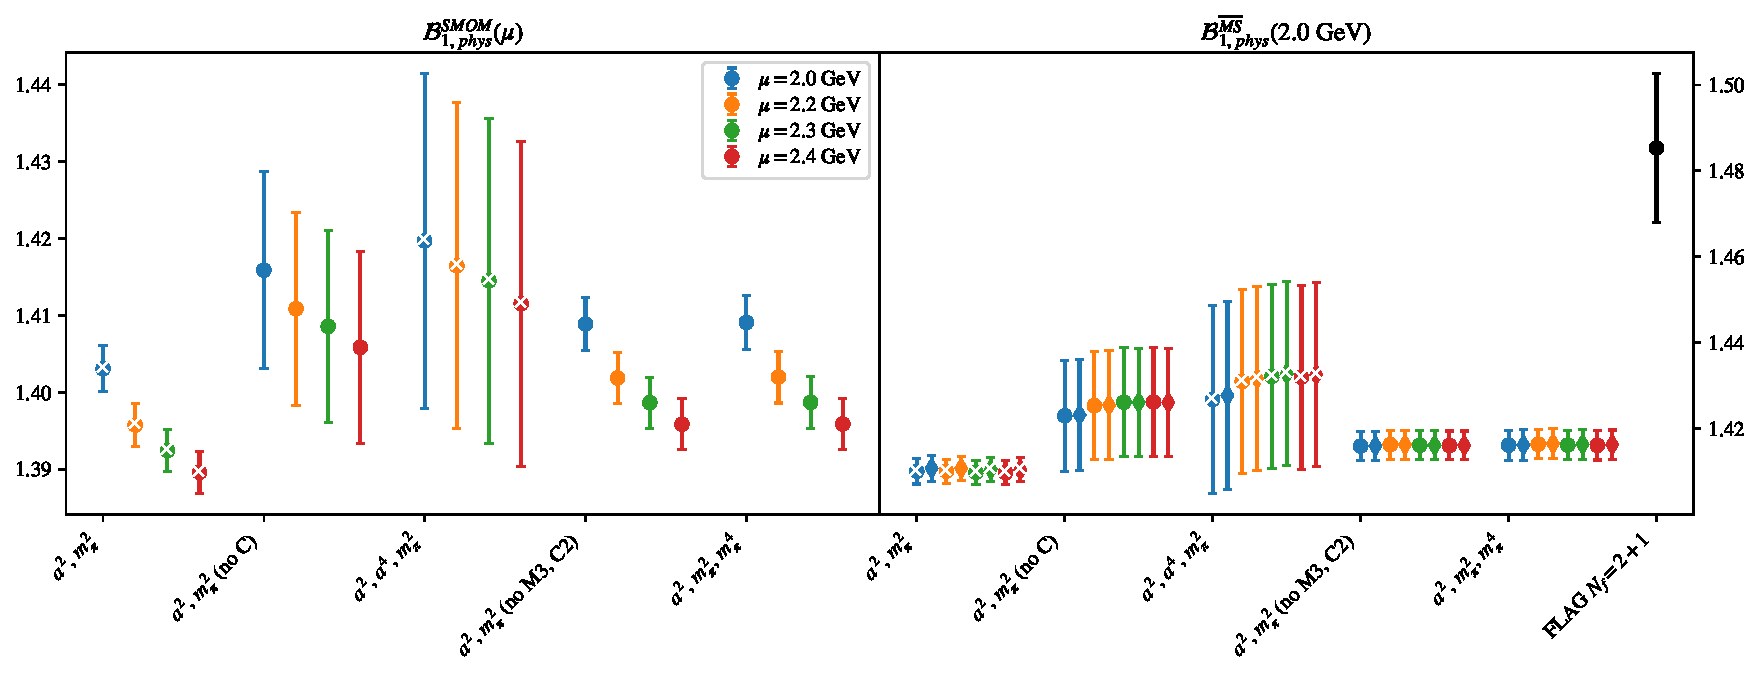
\includegraphics[page=1, width=1.1\textwidth]{VVpAA/SUSY/fit_summary.pdf}
\caption{$B_{1}$\\(left) $B_{phys}$ in RI/SMOM scheme from fit variations (fits with $p$-value $<0.05$ marked with ``$\times$"). \\(right) $B_{phys}$ in $\overline{MS}$ computed using $B^{\overline{MS}} = R^{\overline{MS}\leftarrow SMOM}(2.0)\sigma_{npt}(2.0,\mu) B^{SMOM}(\mu)$.}
\end{figure}
\clearpage
\begin{figure}
\centering
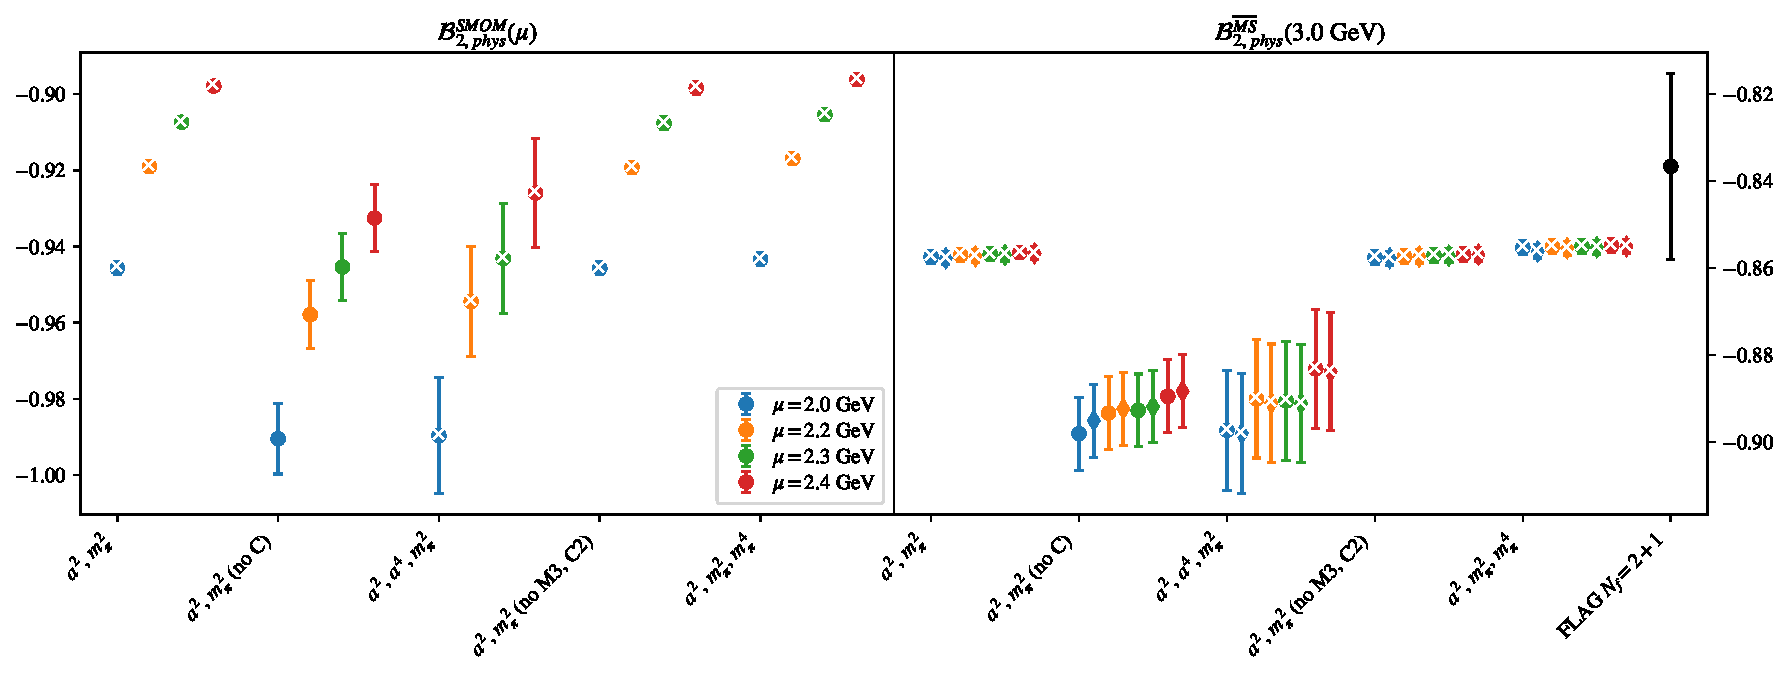
\includegraphics[page=1, width=1.1\textwidth]{VVmAA/SUSY/fit_summary.pdf}
\caption{$B_{2}$\\(left) $B_{phys}$ in RI/SMOM scheme from fit variations (fits with $p$-value $<0.05$ marked with ``$\times$"). \\(right) $B_{phys}$ in $\overline{MS}$ computed using $B^{\overline{MS}} = R^{\overline{MS}\leftarrow SMOM}(3.0)\sigma_{npt}(3.0,\mu) B^{SMOM}(\mu)$.}
\end{figure}
\clearpage
\begin{figure}
\centering
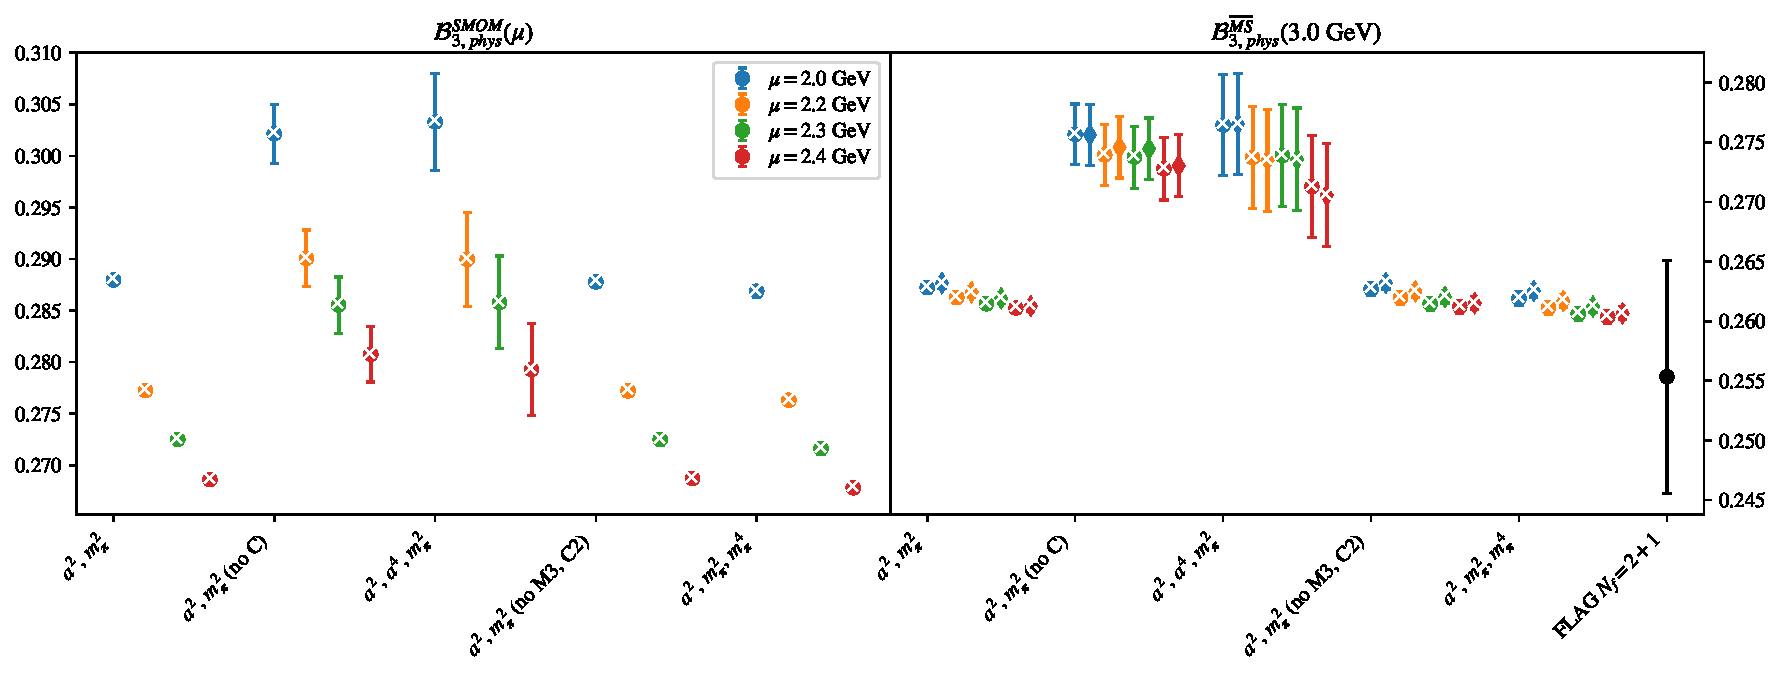
\includegraphics[page=1, width=1.1\textwidth]{SSmPP/SUSY/fit_summary.pdf}
\caption{$B_{3}$\\(left) $B_{phys}$ in RI/SMOM scheme from fit variations (fits with $p$-value $<0.05$ marked with ``$\times$"). \\(right) $B_{phys}$ in $\overline{MS}$ computed using $B^{\overline{MS}} = R^{\overline{MS}\leftarrow SMOM}(3.0)\sigma_{npt}(3.0,\mu) B^{SMOM}(\mu)$.}
\end{figure}
\clearpage
\begin{figure}
\centering
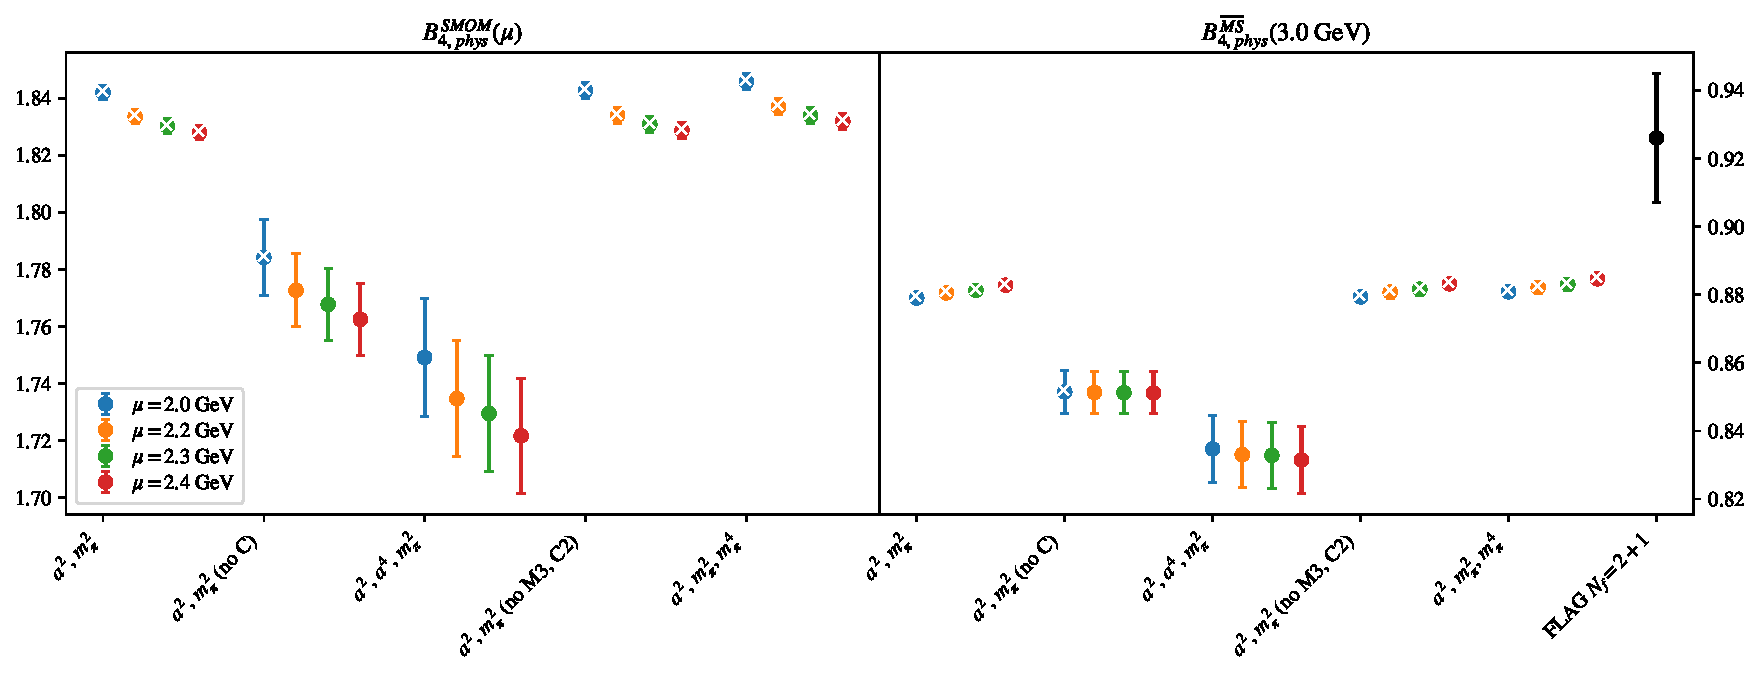
\includegraphics[page=1, width=1.1\textwidth]{SSpPP/SUSY/fit_summary.pdf}
\caption{$B_{4}$\\(left) $B_{phys}$ in RI/SMOM scheme from fit variations (fits with $p$-value $<0.05$ marked with ``$\times$"). \\(right) $B_{phys}$ in $\overline{MS}$ computed using $B^{\overline{MS}} = R^{\overline{MS}\leftarrow SMOM}(3.0)\sigma_{npt}(3.0,\mu) B^{SMOM}(\mu)$.}
\end{figure}
\clearpage
\begin{figure}
\centering
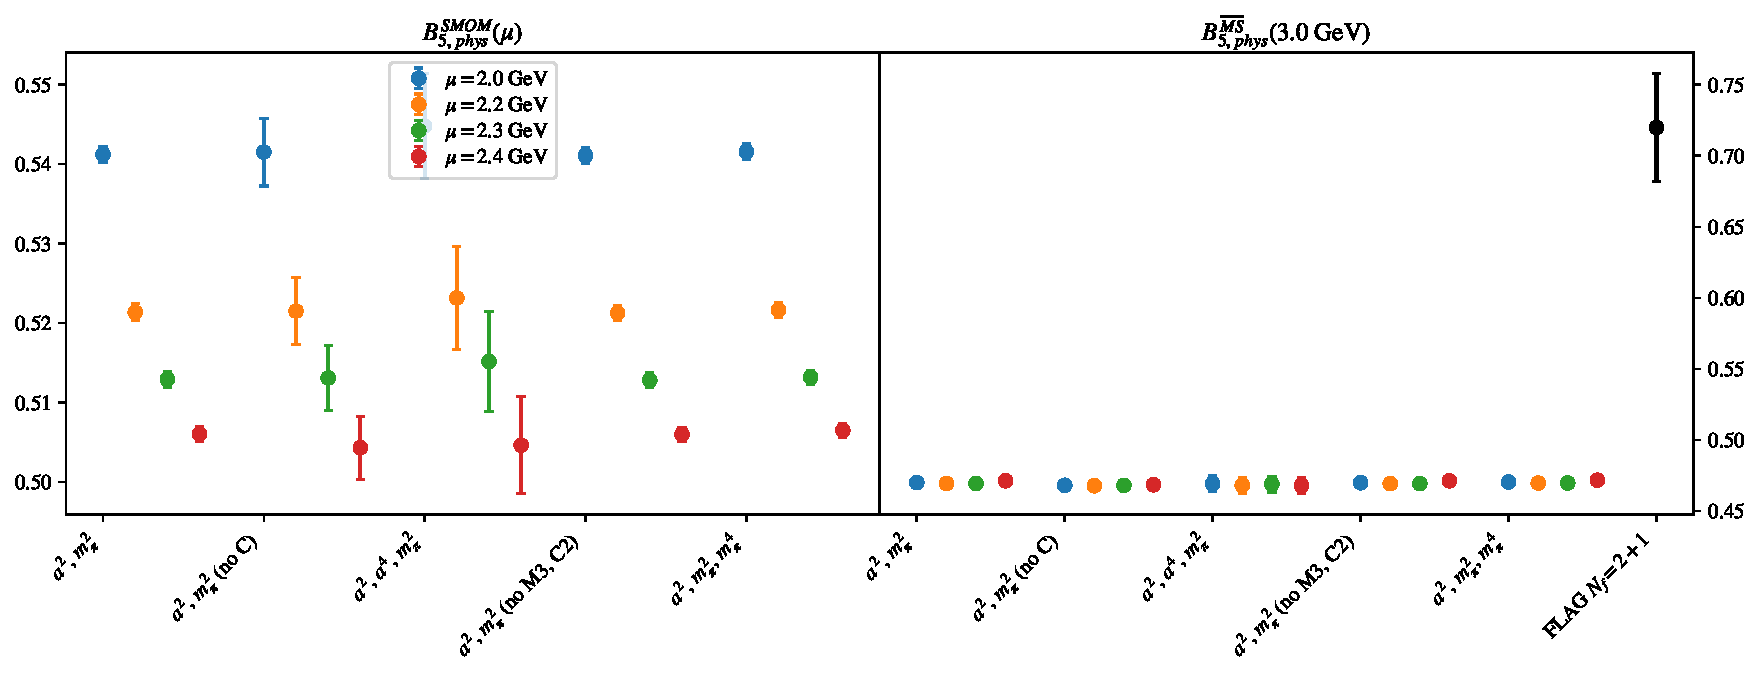
\includegraphics[page=1, width=1.1\textwidth]{TT/SUSY/fit_summary.pdf}
\caption{$B_{5}$\\(left) $B_{phys}$ in RI/SMOM scheme from fit variations (fits with $p$-value $<0.05$ marked with ``$\times$"). \\(right) $B_{phys}$ in $\overline{MS}$ computed using $B^{\overline{MS}} = R^{\overline{MS}\leftarrow SMOM}(3.0)\sigma_{npt}(3.0,\mu) B^{SMOM}(\mu)$.}
\end{figure}
\clearpage
\section{$B_1$}
\begin{table}[h!]
\begin{center}
\begin{tabular}{|c|c|c|c|c|c|}
\hline
$\mu$ (GeV) & $a^2$, $m_\pi^2$& $a^2$, $m_\pi^2$ (no C)& $a^2$, $a^4$, $m_\pi^2$& $a^2$, $m_\pi^2$ (no M3, C2)& $a^2$, $m_\pi^2$, $m_\pi^4$\\
\hline
2.0& \hyperlink{VVpAA/SUSY/a2m2_20.pdf.1}{\textbf{1.4037(28)}: 1.858 (0.098)} & \hyperlink{VVpAA/SUSY/a2m2noC_20.pdf.1}{\textbf{1.416(12)}: 0.876 (0.417)} & \hyperlink{VVpAA/SUSY/a2a4m2_20.pdf.1}{\textbf{1.420(21)}: 2.173 (0.069)} & \hyperlink{VVpAA/SUSY/a2m2mcut_20.pdf.1}{\textbf{1.4089(33)}: 0.248 (0.863)} & \hyperlink{VVpAA/SUSY/a2m2m4_20.pdf.1}{\textbf{1.4091(34)}: 0.661 (0.619)}\\
2.2& \hyperlink{VVpAA/SUSY/a2m2_22.pdf.1}{\textbf{1.3964(27)}: 2.214 (0.05)} & \hyperlink{VVpAA/SUSY/a2m2noC_22.pdf.1}{\textbf{1.411(12)}: 1.143 (0.319)} & \hyperlink{VVpAA/SUSY/a2a4m2_22.pdf.1}{\textbf{1.417(21)}: 2.525 (0.039)} & \hyperlink{VVpAA/SUSY/a2m2mcut_22.pdf.1}{\textbf{1.4018(32)}: 0.36 (0.782)} & \hyperlink{VVpAA/SUSY/a2m2m4_22.pdf.1}{\textbf{1.4021(33)}: 0.923 (0.449)}\\
2.3& \hyperlink{VVpAA/SUSY/a2m2_23.pdf.1}{\textbf{1.3931(26)}: 2.304 (0.042)} & \hyperlink{VVpAA/SUSY/a2m2noC_23.pdf.1}{\textbf{1.408(12)}: 1.197 (0.302)} & \hyperlink{VVpAA/SUSY/a2a4m2_23.pdf.1}{\textbf{1.415(21)}: 2.605 (0.034)} & \hyperlink{VVpAA/SUSY/a2m2mcut_23.pdf.1}{\textbf{1.3986(32)}: 0.411 (0.745)} & \hyperlink{VVpAA/SUSY/a2m2m4_23.pdf.1}{\textbf{1.3988(33)}: 0.993 (0.41)}\\
2.4& \hyperlink{VVpAA/SUSY/a2m2_24.pdf.1}{\textbf{1.3902(26)}: 2.348 (0.039)} & \hyperlink{VVpAA/SUSY/a2m2noC_24.pdf.1}{\textbf{1.405(12)}: 1.223 (0.294)} & \hyperlink{VVpAA/SUSY/a2a4m2_24.pdf.1}{\textbf{1.412(21)}: 2.663 (0.031)} & \hyperlink{VVpAA/SUSY/a2m2mcut_24.pdf.1}{\textbf{1.3958(32)}: 0.411 (0.745)} & \hyperlink{VVpAA/SUSY/a2m2m4_24.pdf.1}{\textbf{1.3960(33)}: 1.005 (0.403)}\\
\hline
\end{tabular}
\caption{Physical point value from chiral and continuum extrapolation at renormalisation scale $\mu$. Entries are \textbf{value(error)}: $\chi^2/\text{DOF}$ ($p$-value).}
\end{center}
\end{table}
\begin{table}[h!]
\begin{center}
\begin{tabular}{|c c|c|c|c|c|c|}
\hline
$\mu$ (GeV) &  & $a^2$, $m_\pi^2$& $a^2$, $m_\pi^2$ (no C)& $a^2$, $a^4$, $m_\pi^2$& $a^2$, $m_\pi^2$ (no M3, C2)& $a^2$, $m_\pi^2$, $m_\pi^4$\\
\hline
\multirow{2}{0.5in}{2.0} & $\alpha$ & 0.0937(71)& 0.047(53)& -0.017& 0.0815(83)& 0.0813(82)\\
 & $\beta$ & 0.00261(14)& 0.00223(27)& 0.00263(15)& 0.00189(28)& 0.00031(90)\\
\hline
\multirow{2}{0.5in}{2.2} & $\alpha$ & 0.0977(70)& 0.041(52)& -0.038& 0.0847(83)& 0.0846(82)\\
 & $\beta$ & 0.00261(14)& 0.00220(27)& 0.00264(14)& 0.00184(28)& 0.00020(89)\\
\hline
\multirow{2}{0.5in}{2.3} & $\alpha$ & 0.0992(70)& 0.039(52)& -0.045& 0.0859(83)& 0.0859(82)\\
 & $\beta$ & 0.00262(14)& 0.00220(27)& 0.00265(14)& 0.00184(28)& 0.00018(89)\\
\hline
\multirow{2}{0.5in}{2.4} & $\alpha$ & 0.0999(70)& 0.040(52)& -0.044& 0.0864(83)& 0.0864(82)\\
 & $\beta$ & 0.00263(14)& 0.00220(27)& 0.00266(14)& 0.00184(28)& 0.00017(89)\\
\hline
\end{tabular}
\caption{Fit values of coefficients in $B = B_{phys} + \mathbf{\alpha} a^2 + \mathbf{\beta}\left(\frac{m_\pi^2}{f_\pi^2}-\frac{m_{\pi,PDG}^2}{f_\pi^2}\right) + \ldots$.}
\end{center}
\end{table}
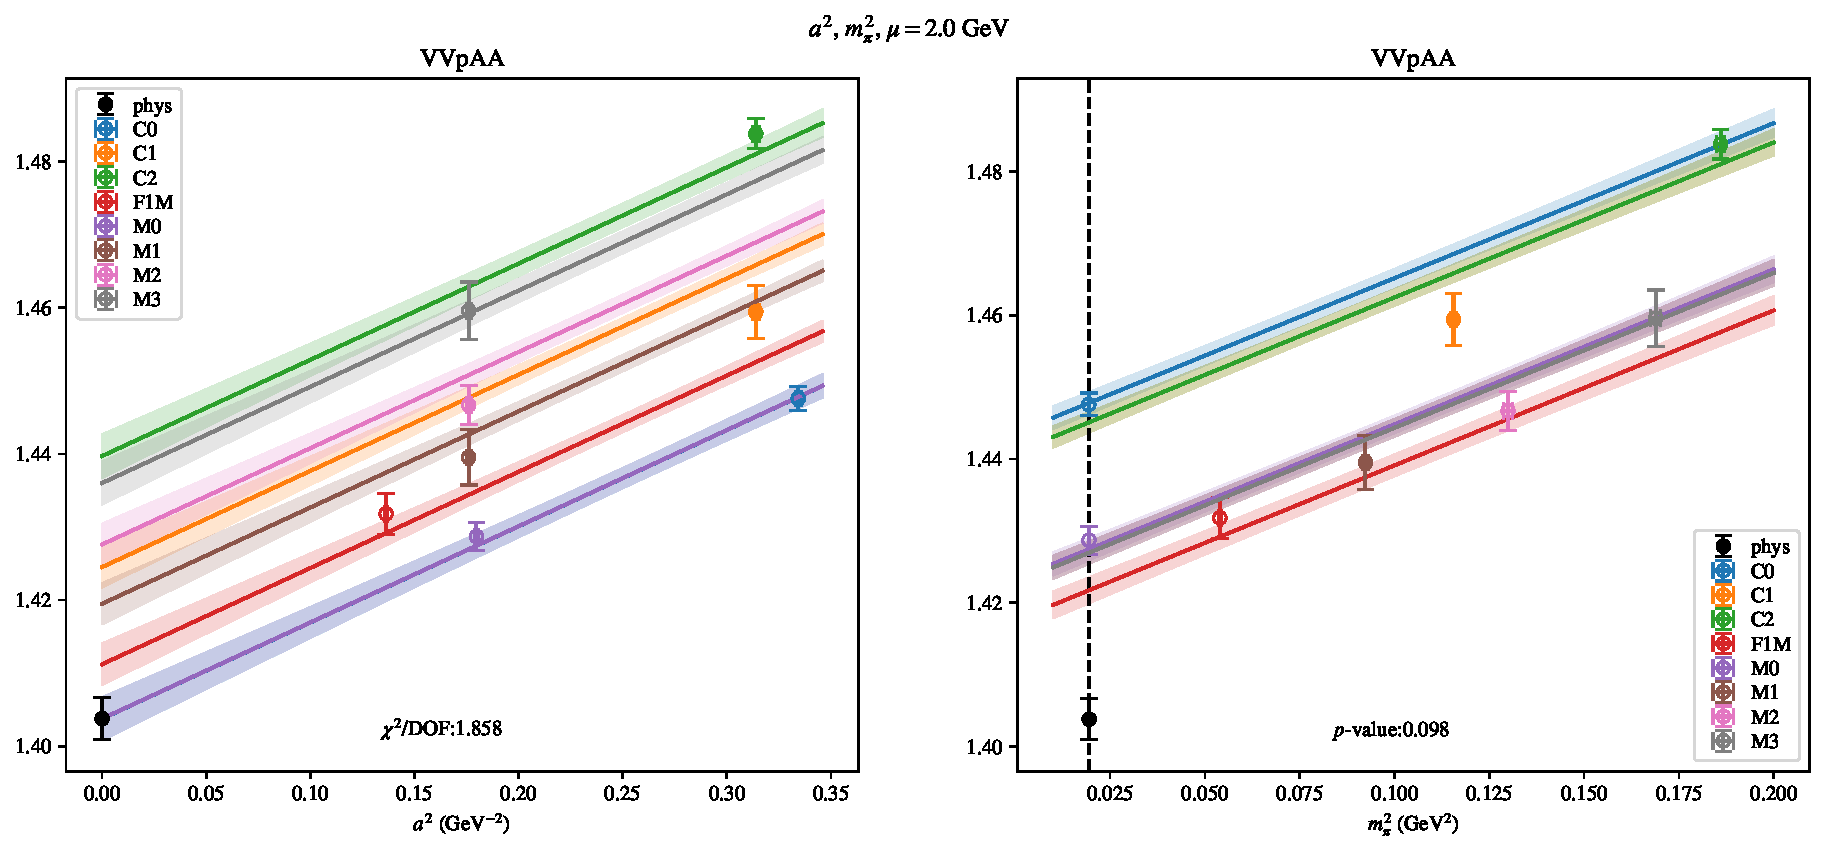
\includepdf[link, pages=-]{VVpAA/SUSY/a2m2_20.pdf}
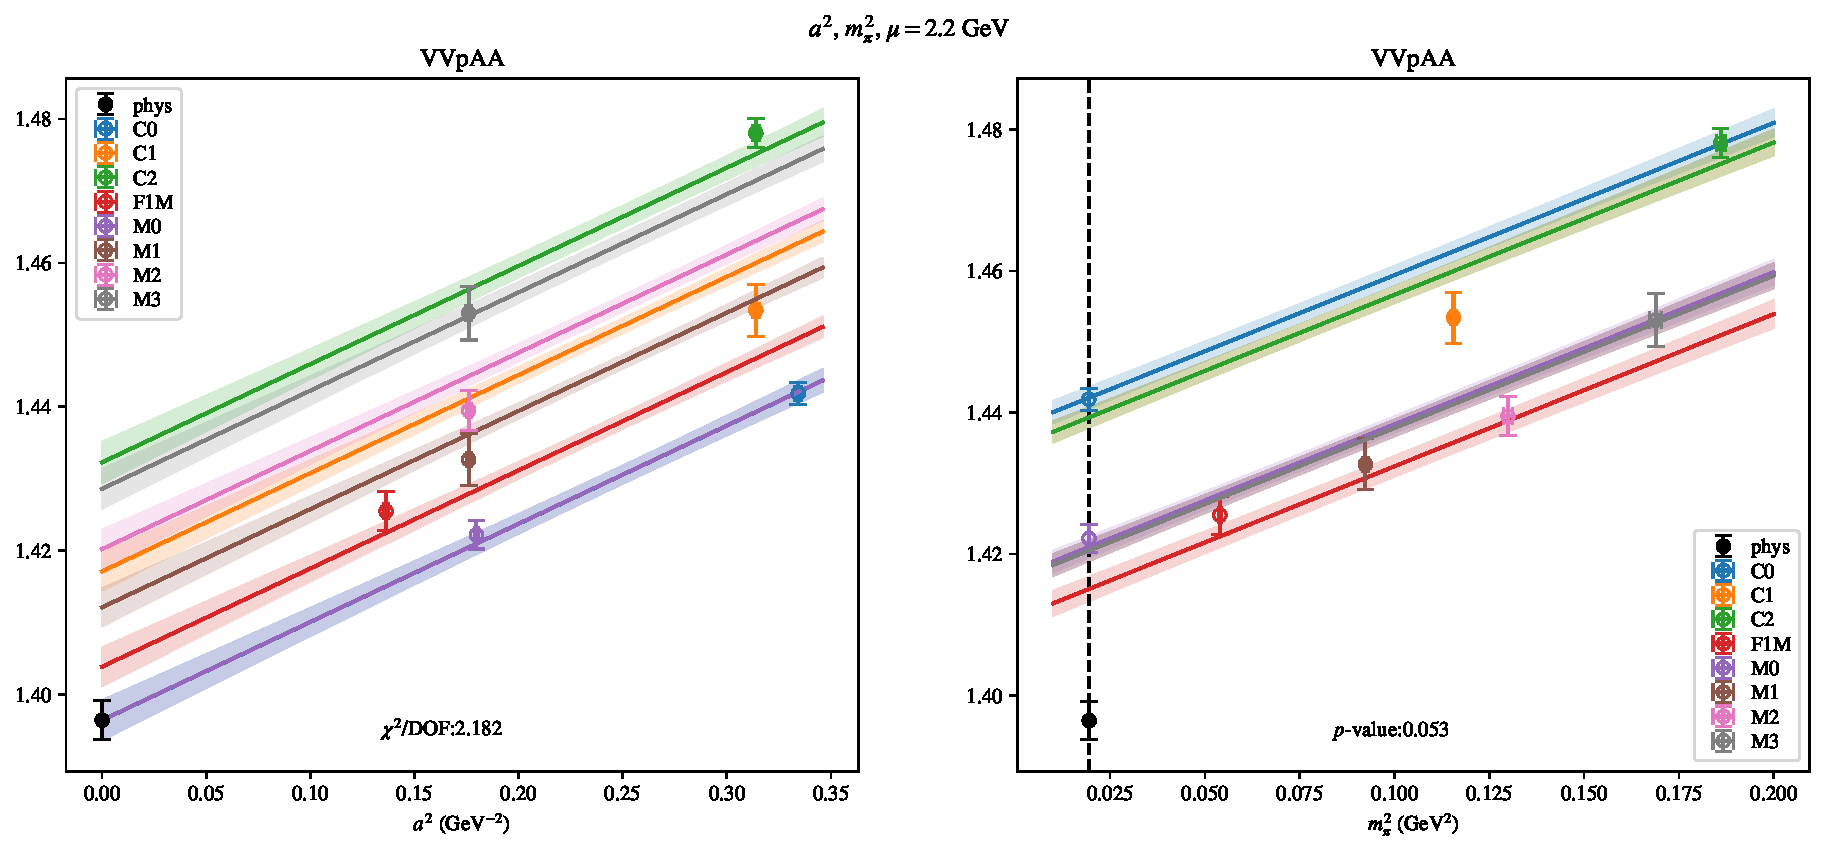
\includepdf[link, pages=-]{VVpAA/SUSY/a2m2_22.pdf}
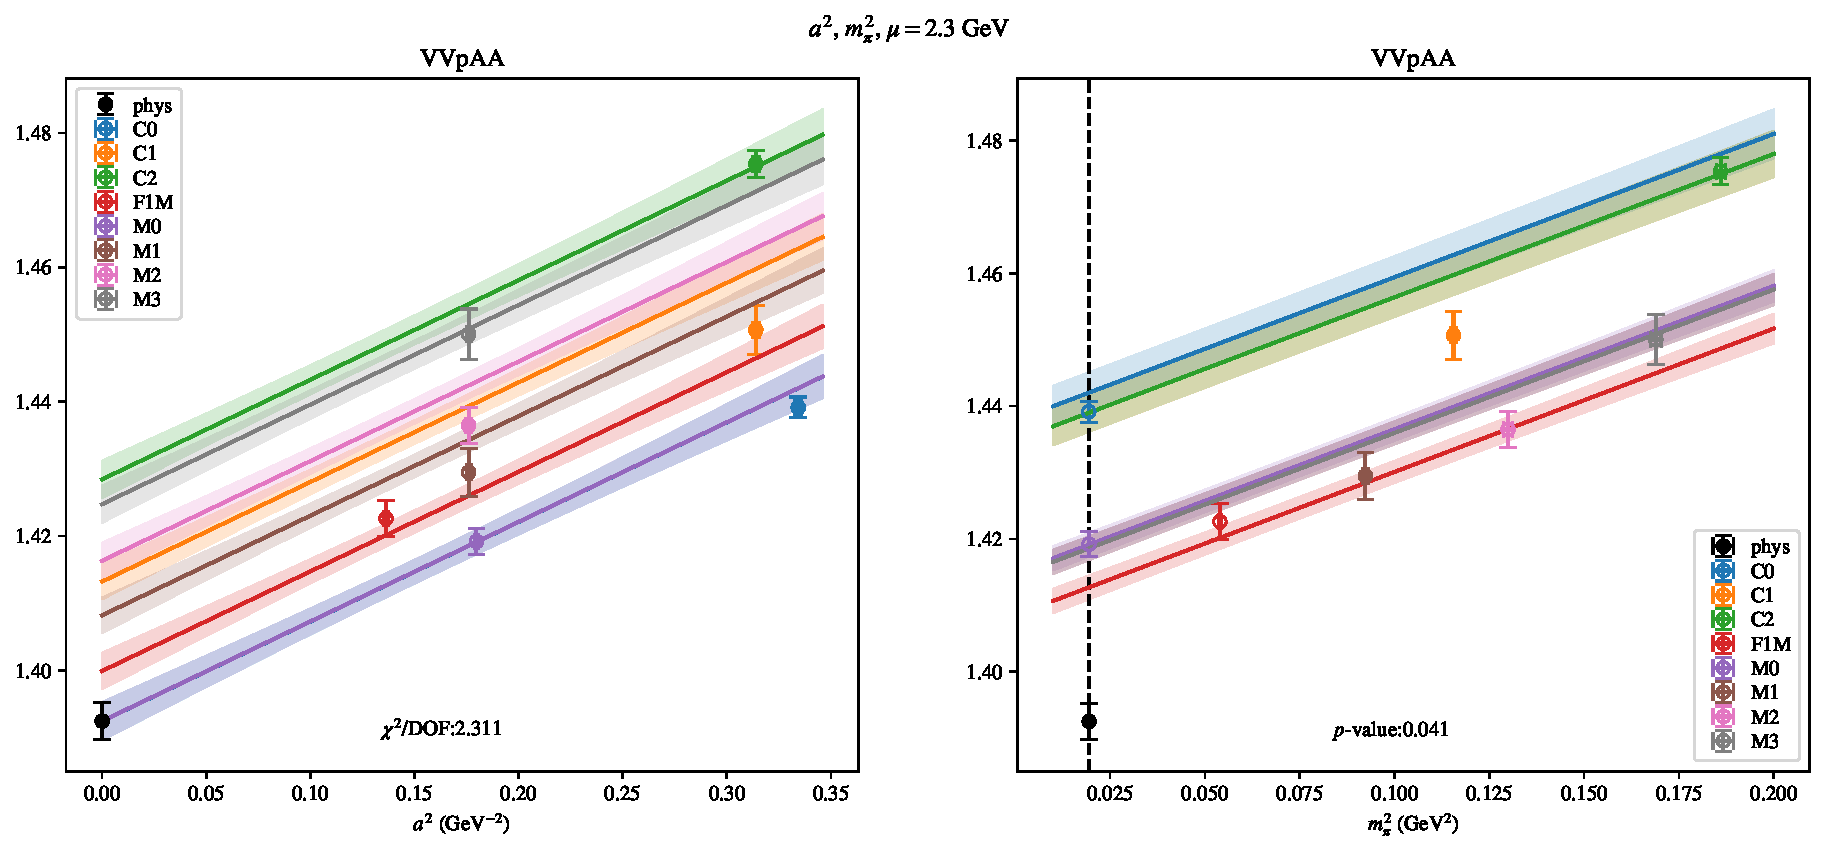
\includepdf[link, pages=-]{VVpAA/SUSY/a2m2_23.pdf}
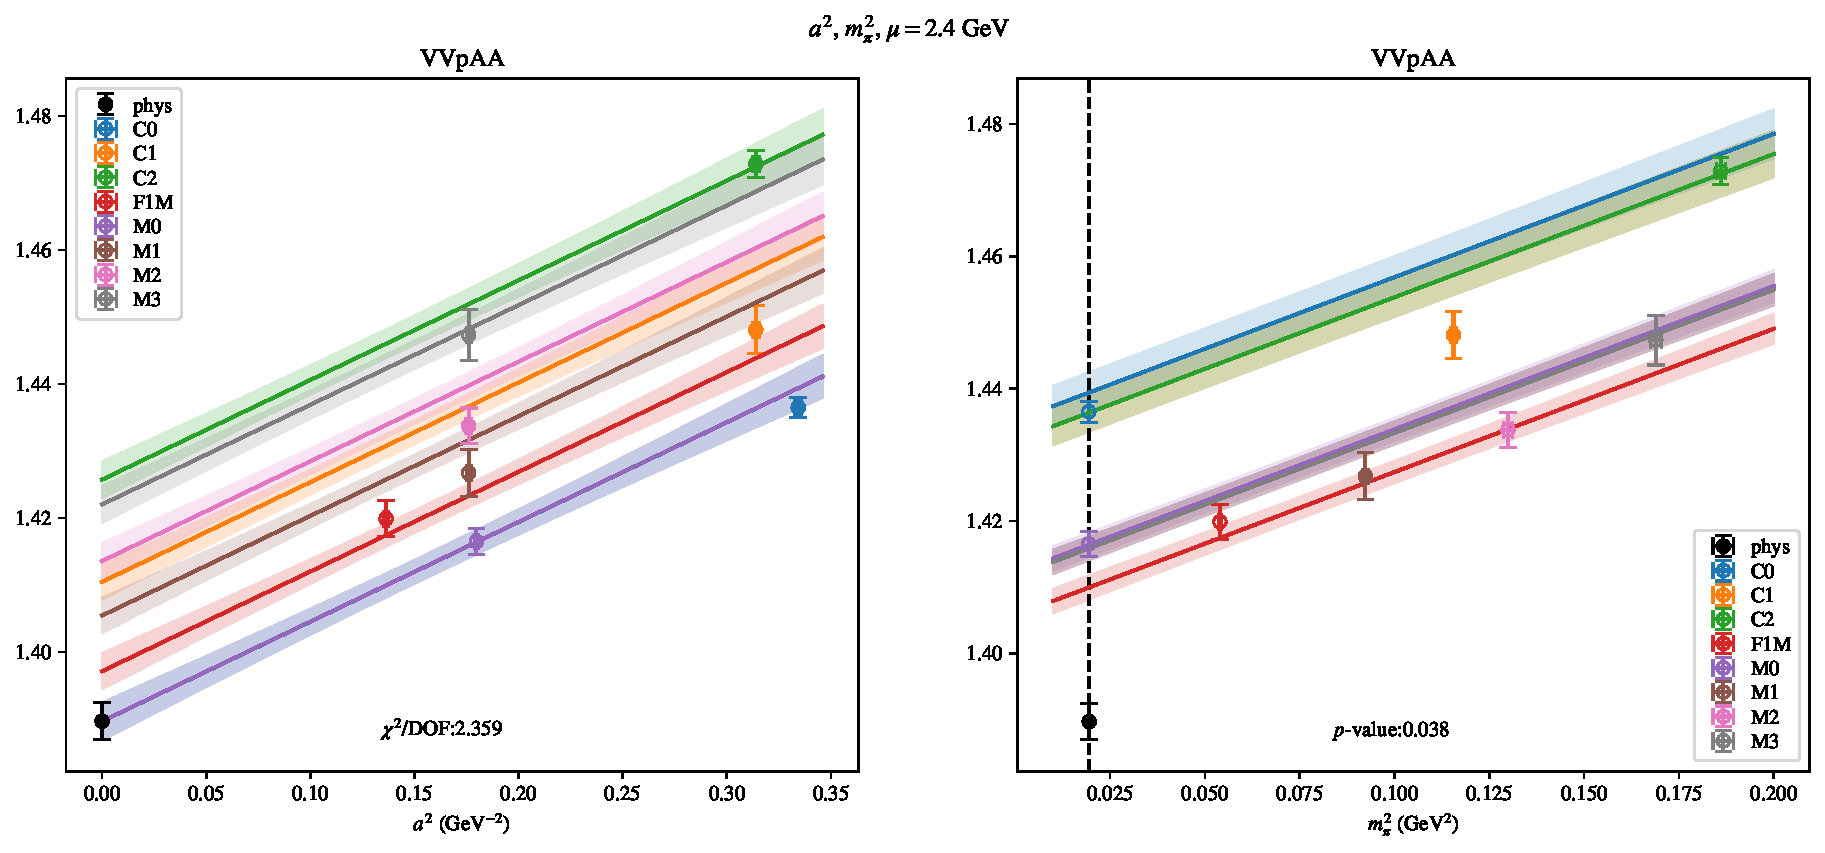
\includepdf[link, pages=-]{VVpAA/SUSY/a2m2_24.pdf}
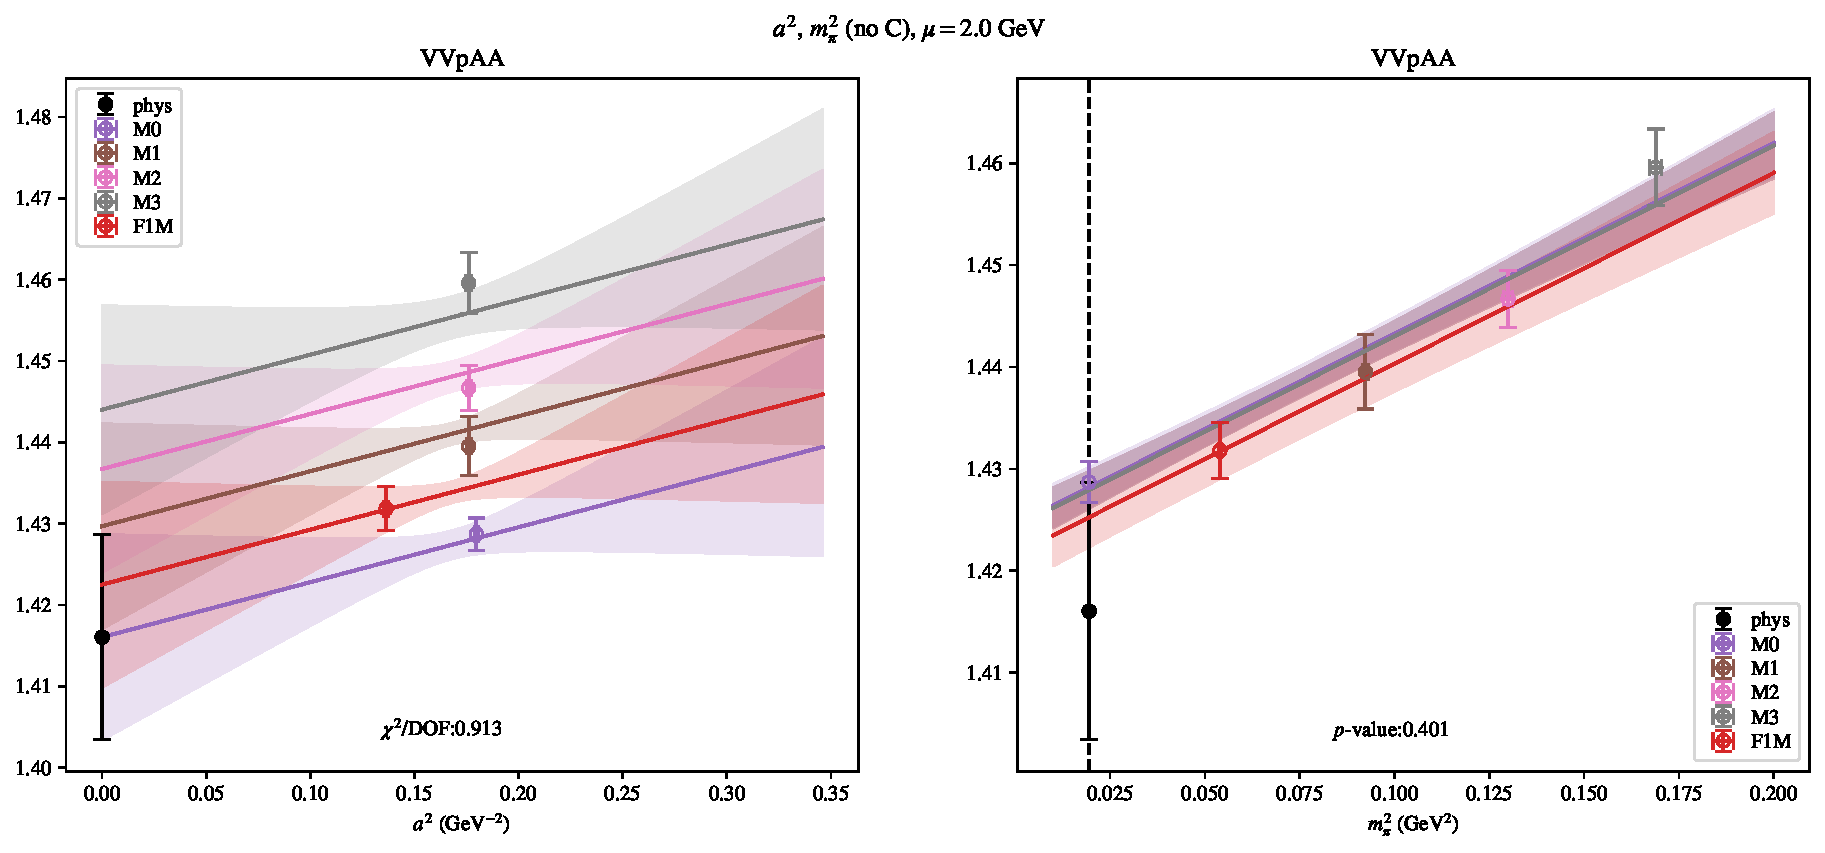
\includepdf[link, pages=-]{VVpAA/SUSY/a2m2noC_20.pdf}
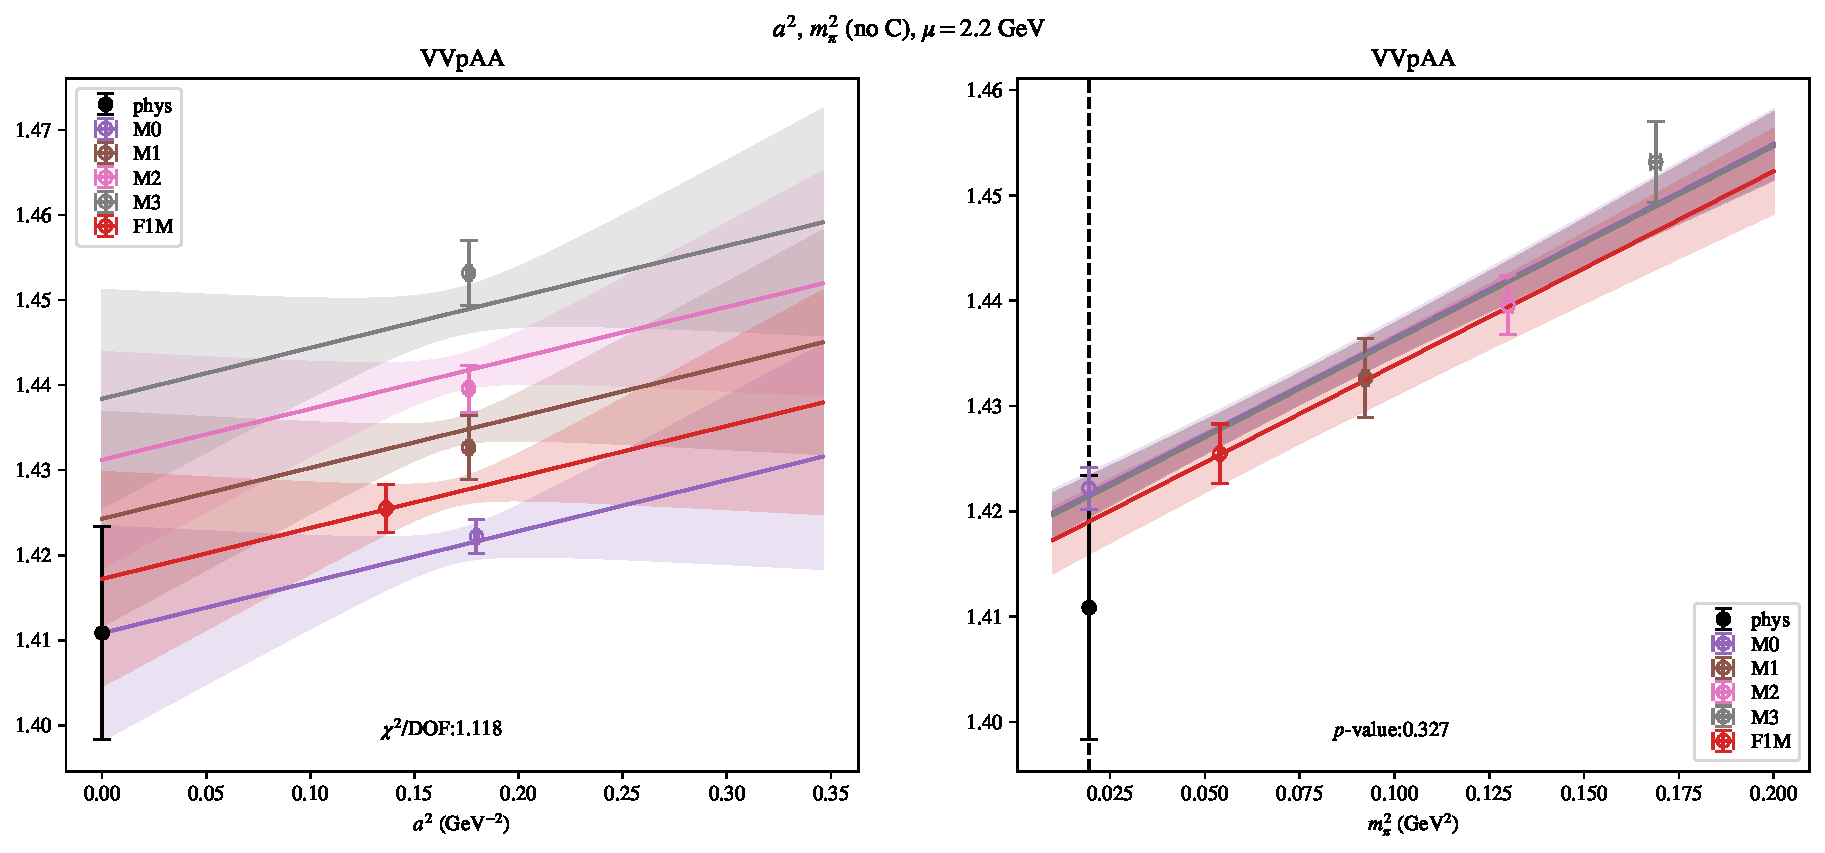
\includepdf[link, pages=-]{VVpAA/SUSY/a2m2noC_22.pdf}
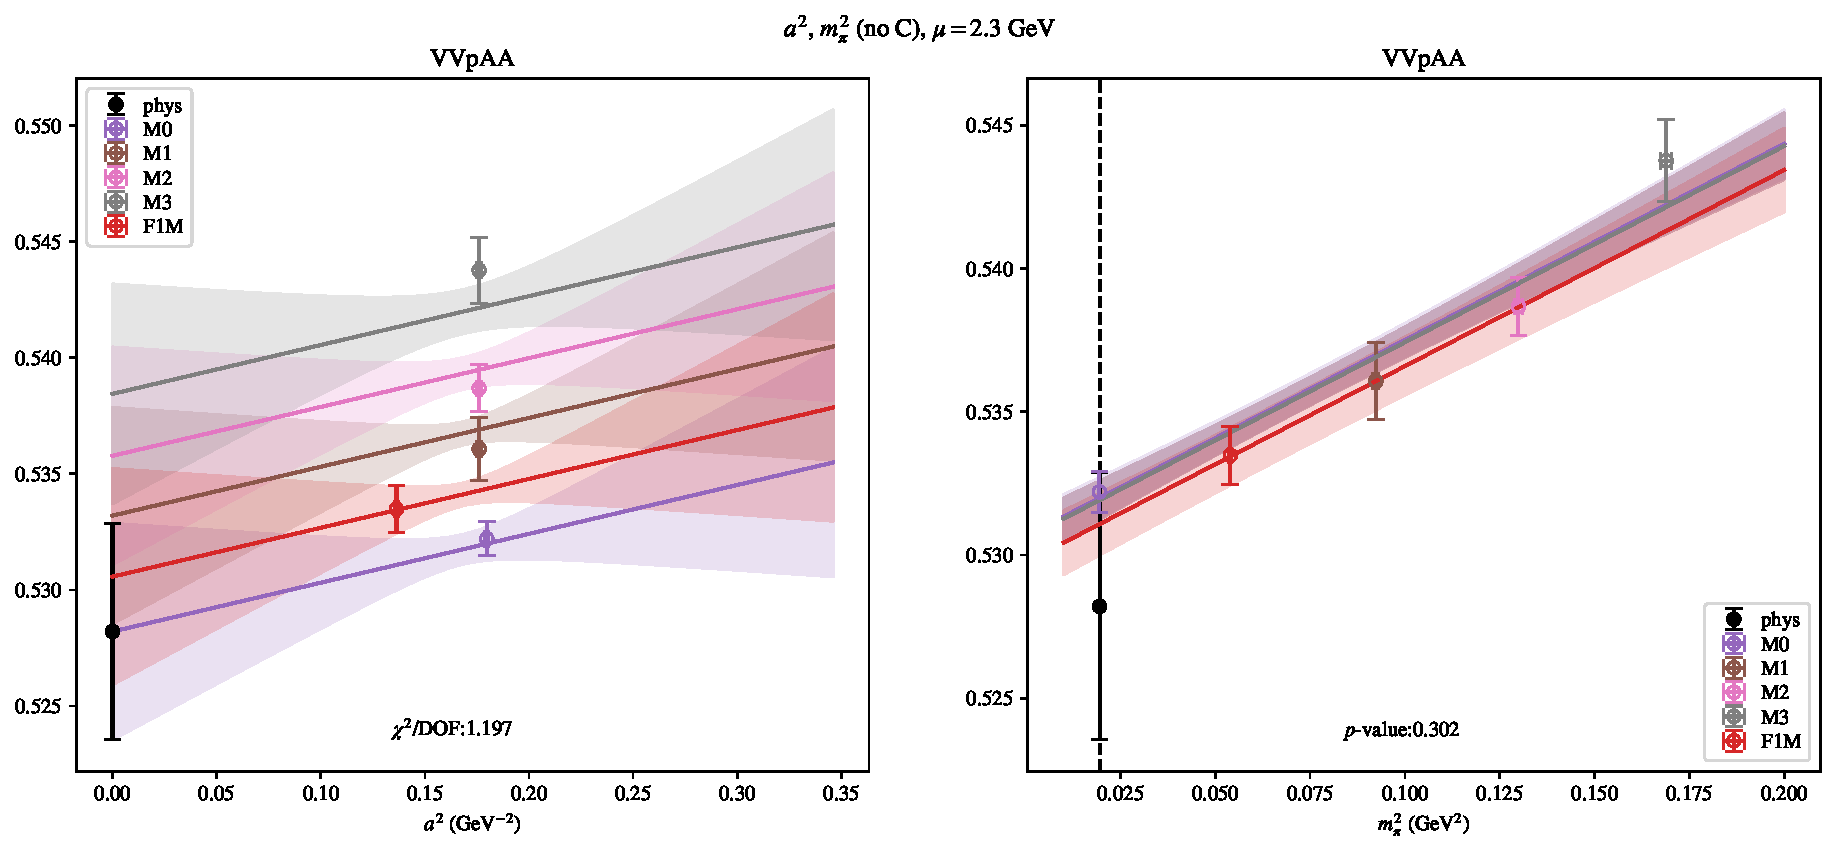
\includepdf[link, pages=-]{VVpAA/SUSY/a2m2noC_23.pdf}
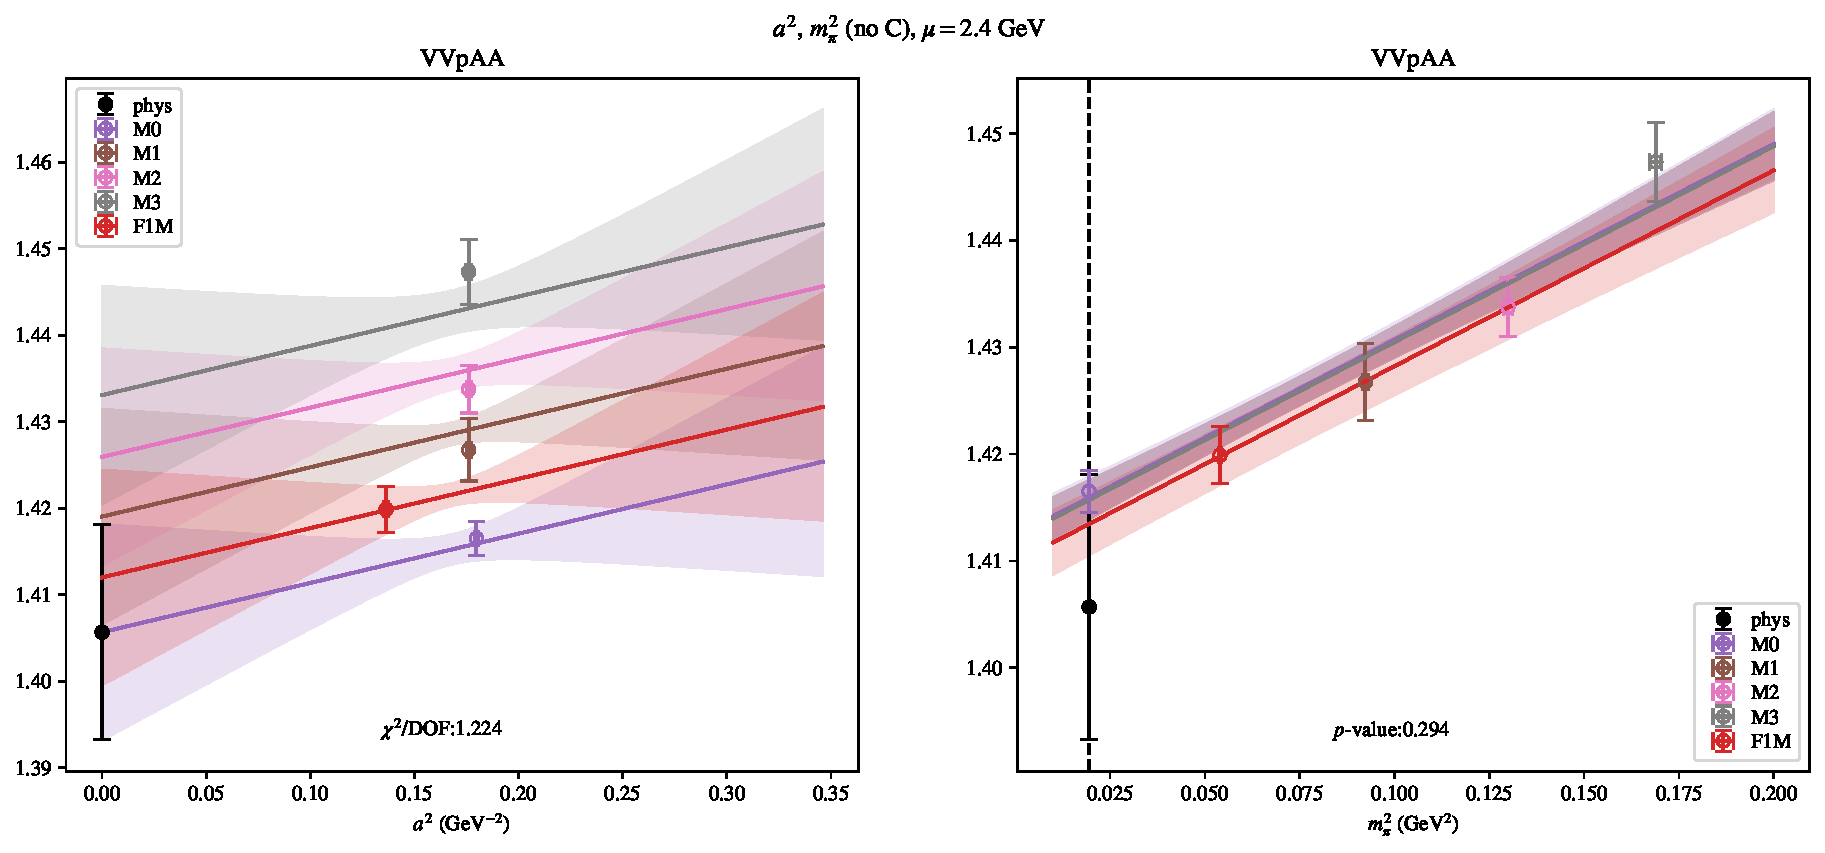
\includepdf[link, pages=-]{VVpAA/SUSY/a2m2noC_24.pdf}
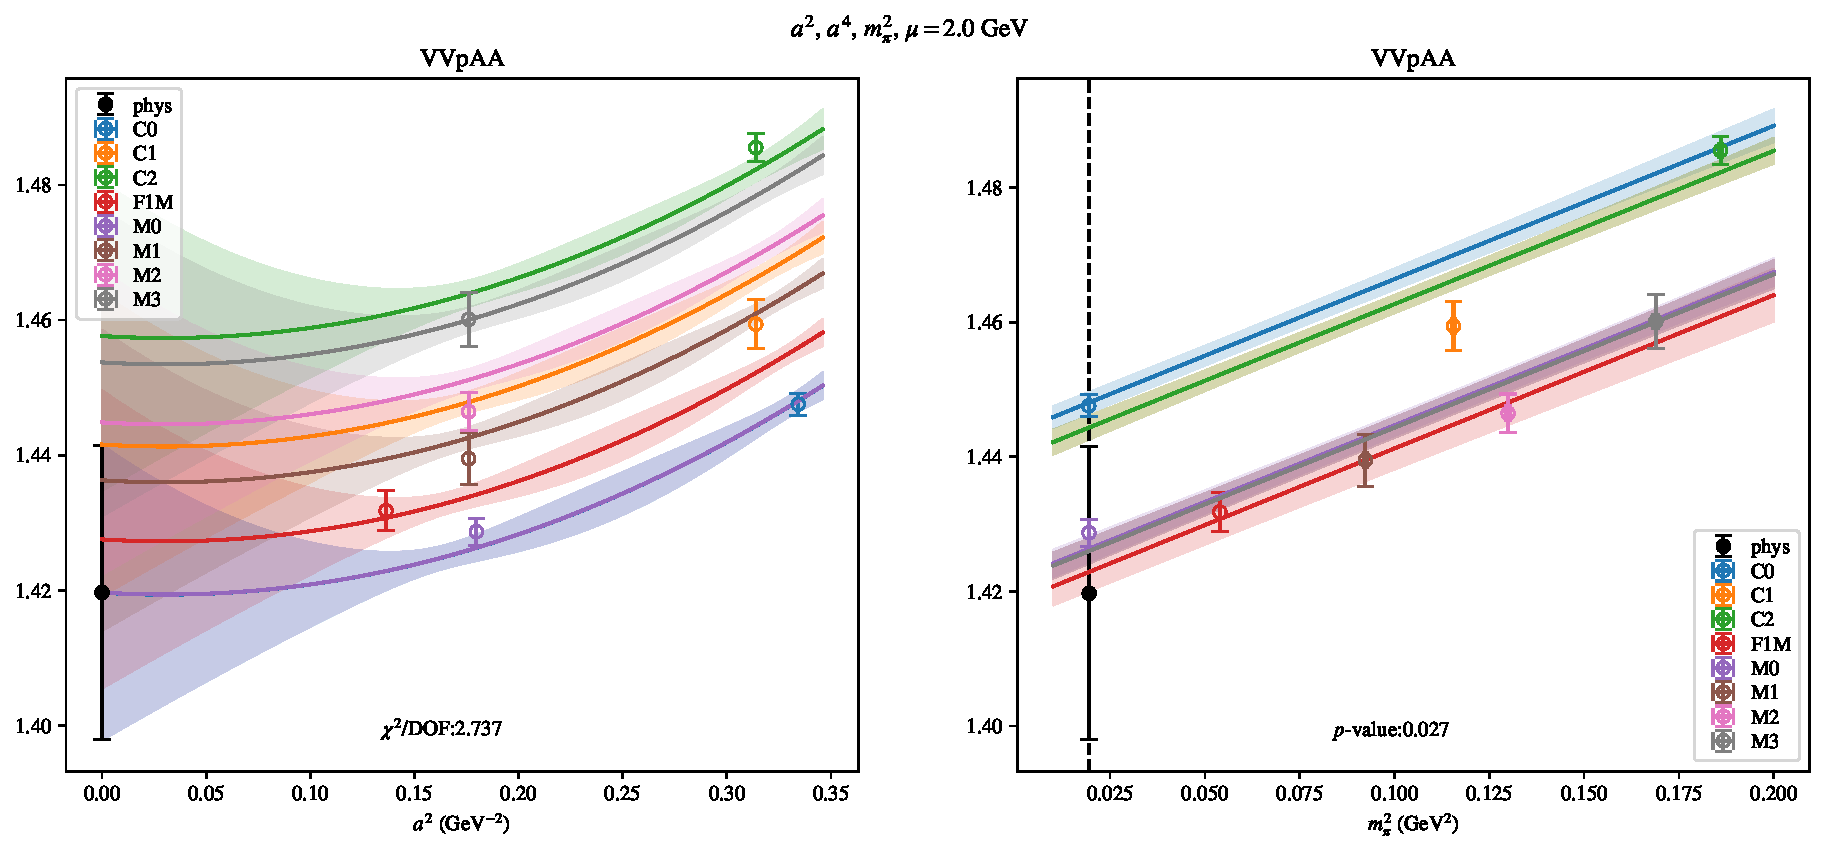
\includepdf[link, pages=-]{VVpAA/SUSY/a2a4m2_20.pdf}
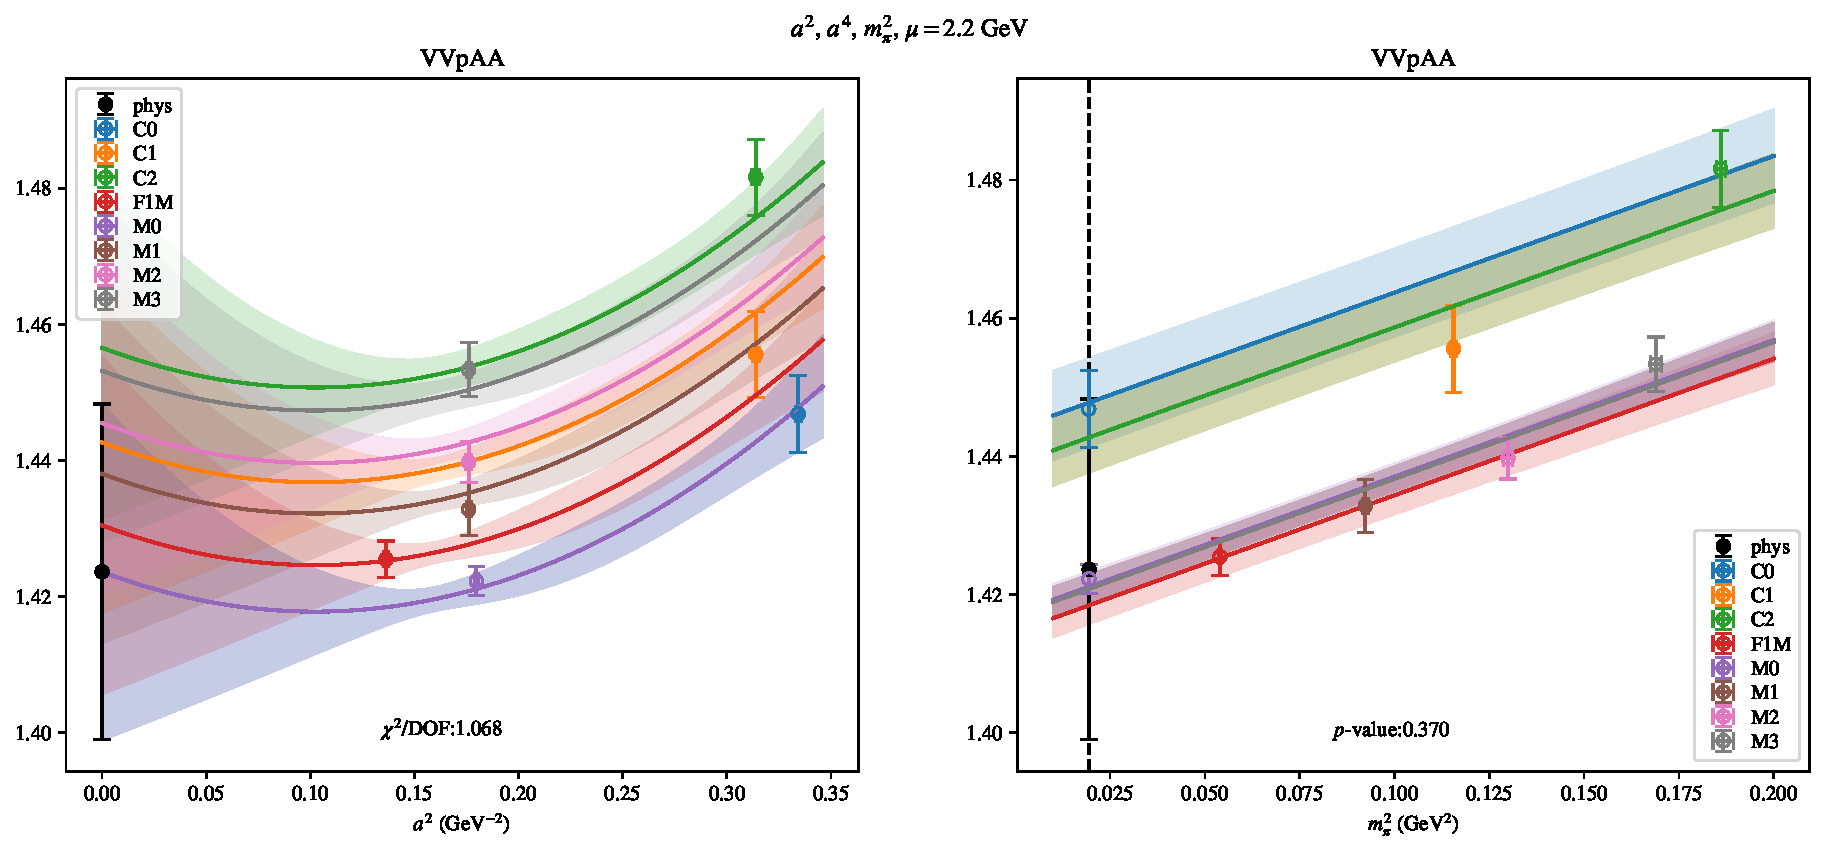
\includepdf[link, pages=-]{VVpAA/SUSY/a2a4m2_22.pdf}
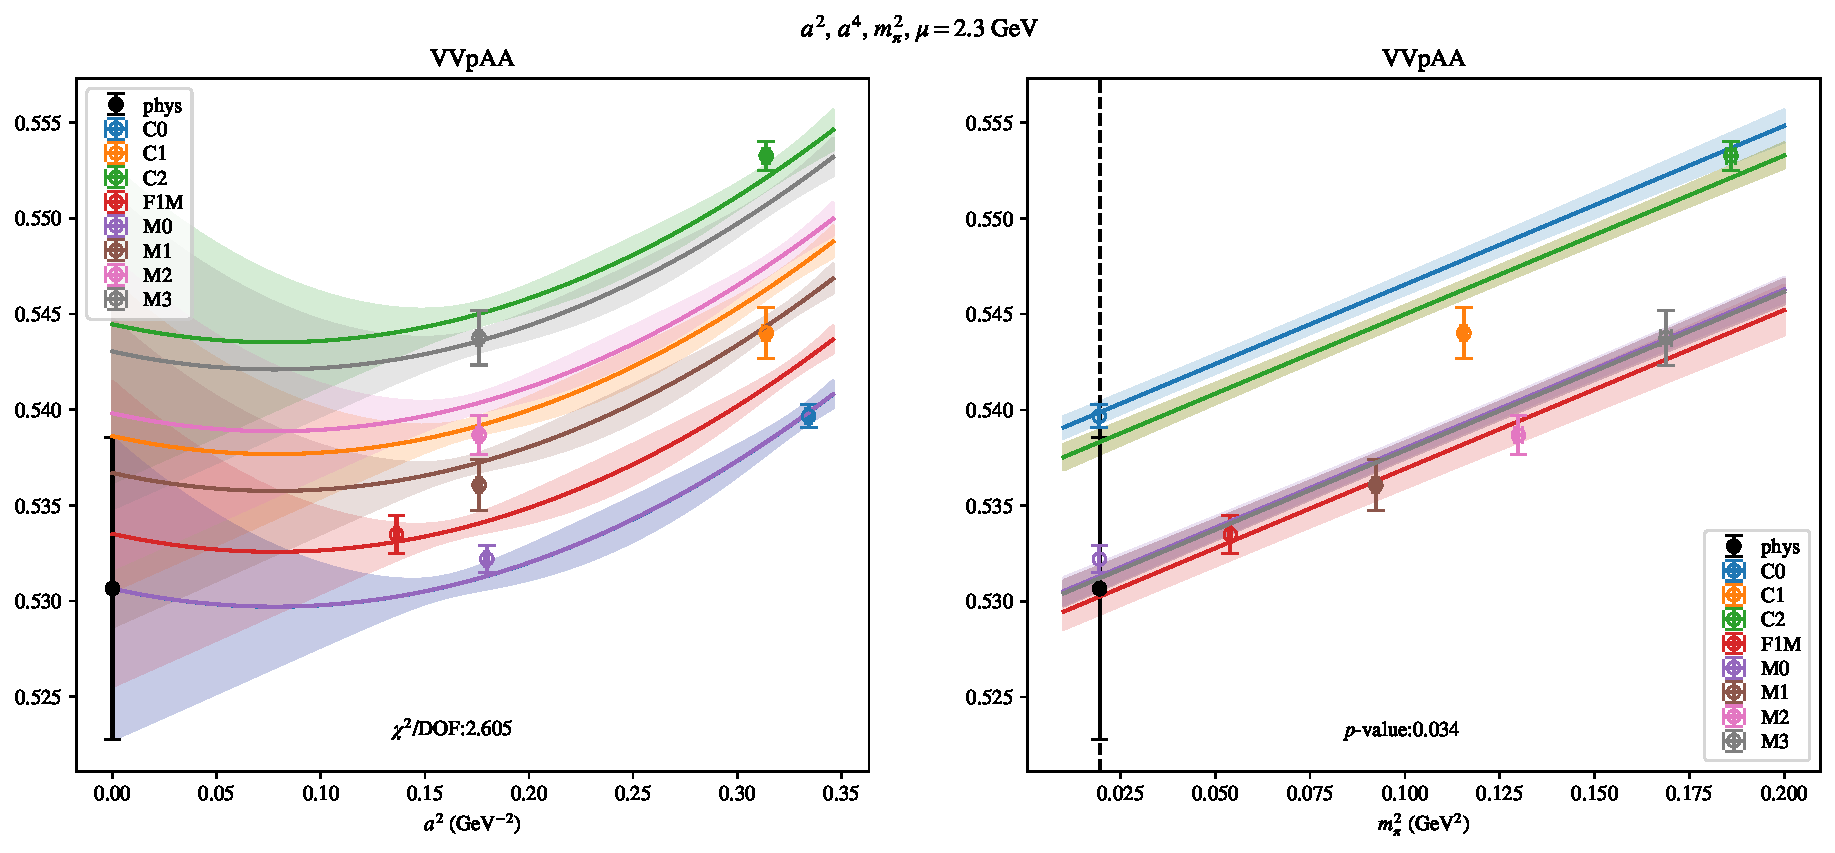
\includepdf[link, pages=-]{VVpAA/SUSY/a2a4m2_23.pdf}
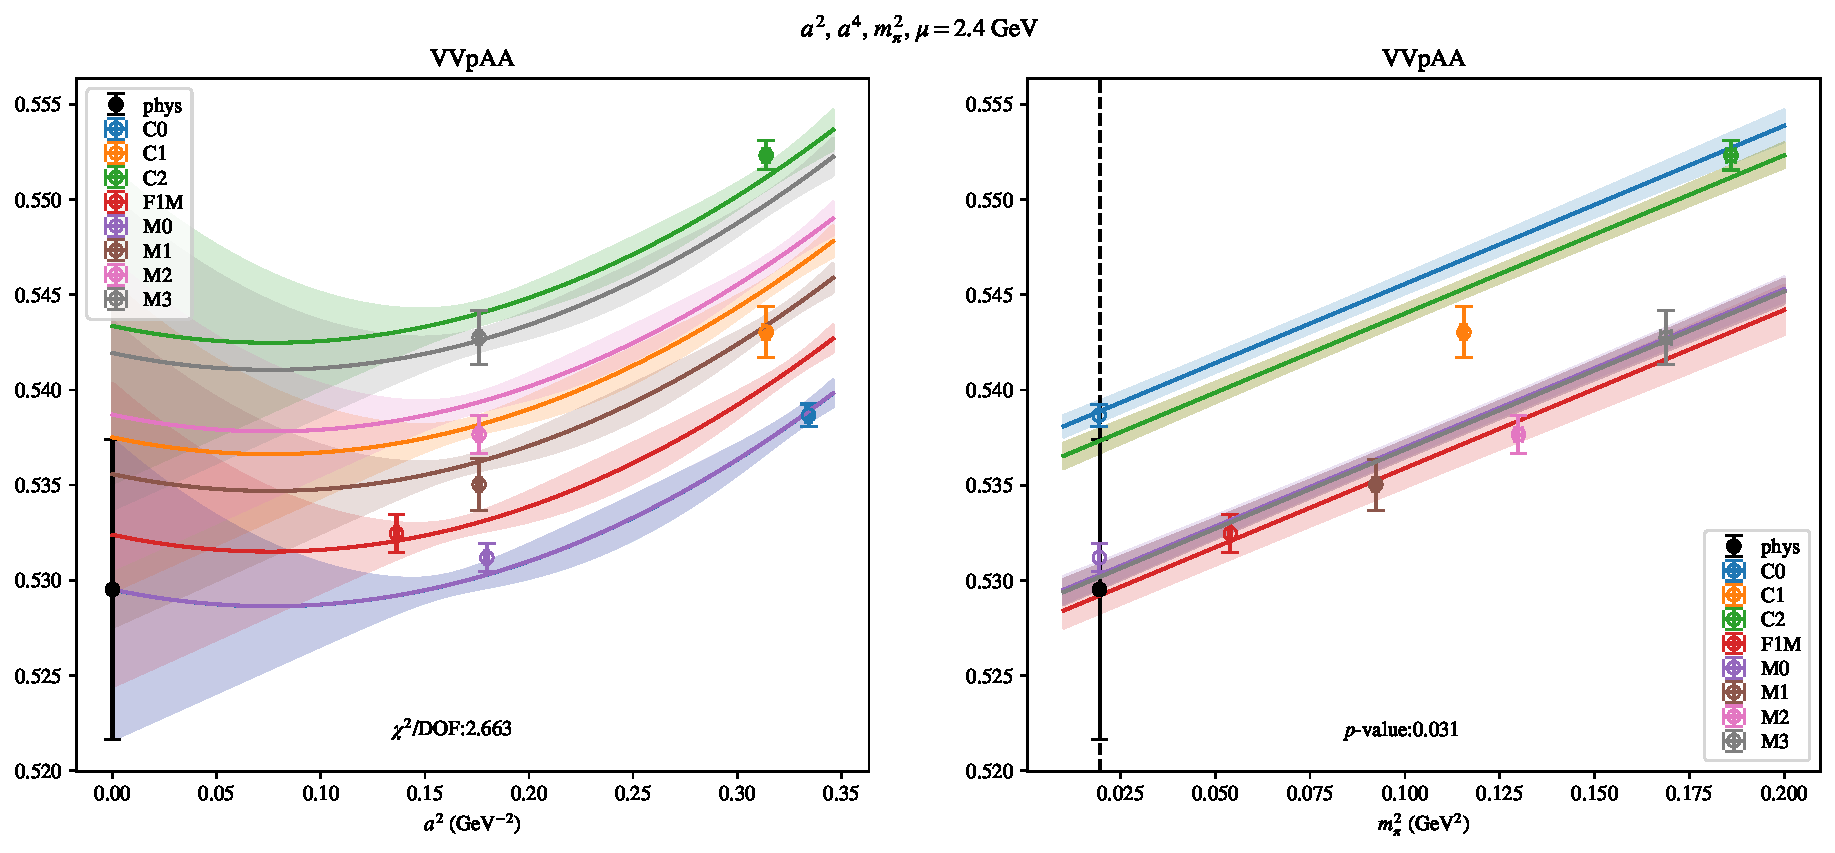
\includepdf[link, pages=-]{VVpAA/SUSY/a2a4m2_24.pdf}
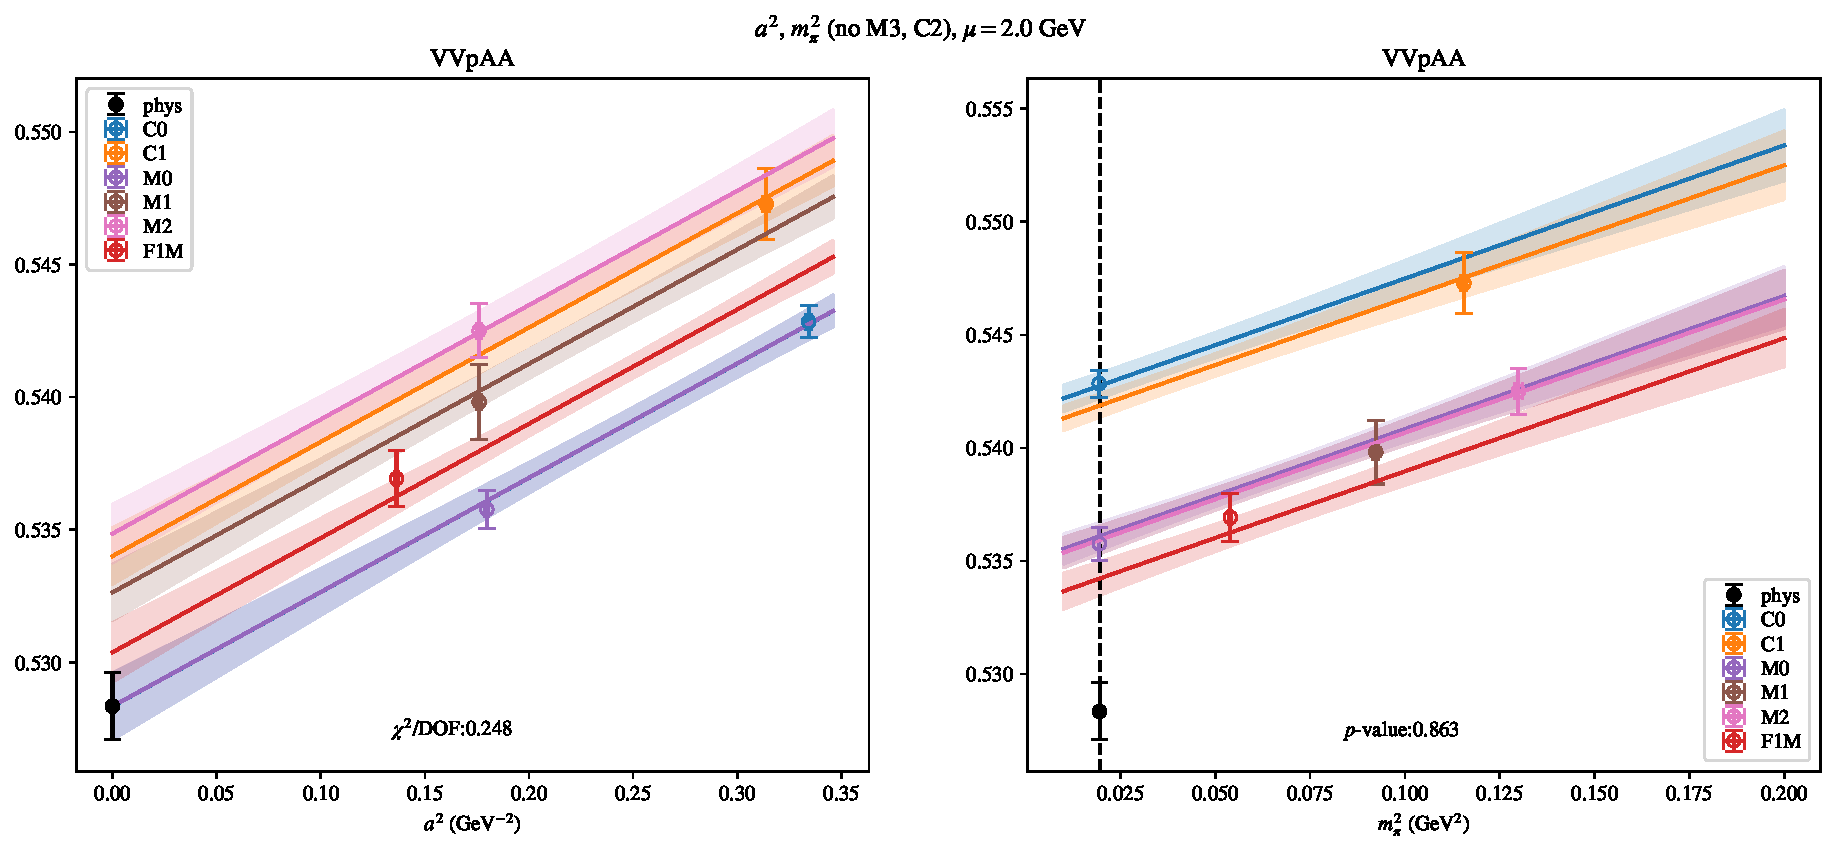
\includepdf[link, pages=-]{VVpAA/SUSY/a2m2mcut_20.pdf}
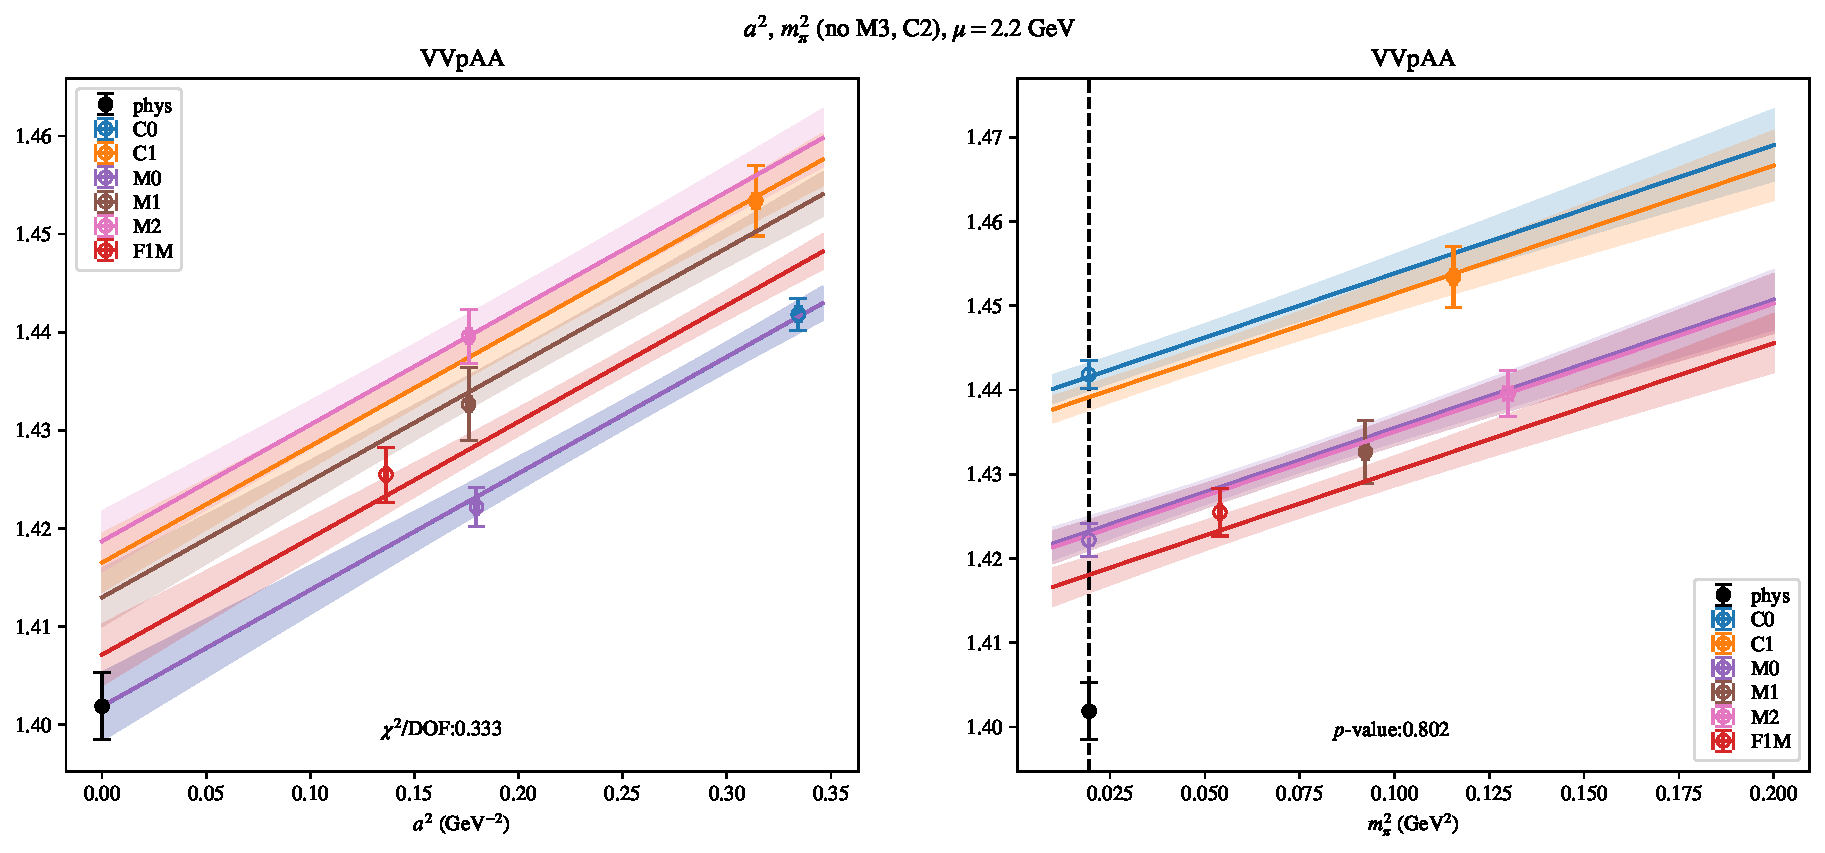
\includepdf[link, pages=-]{VVpAA/SUSY/a2m2mcut_22.pdf}
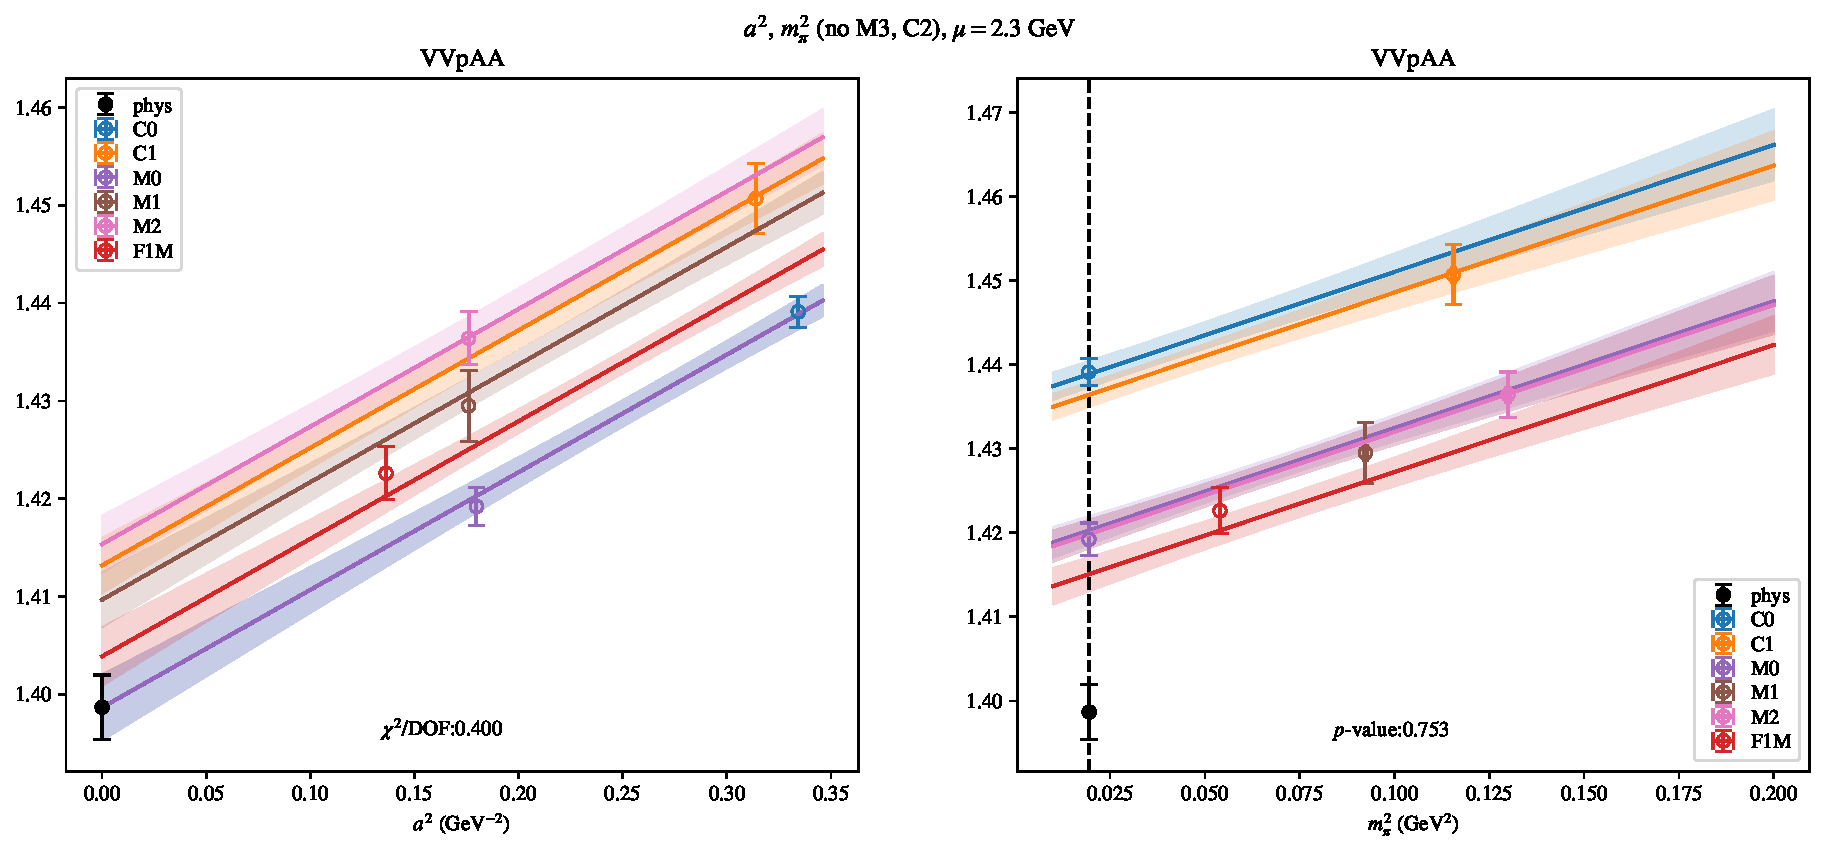
\includepdf[link, pages=-]{VVpAA/SUSY/a2m2mcut_23.pdf}
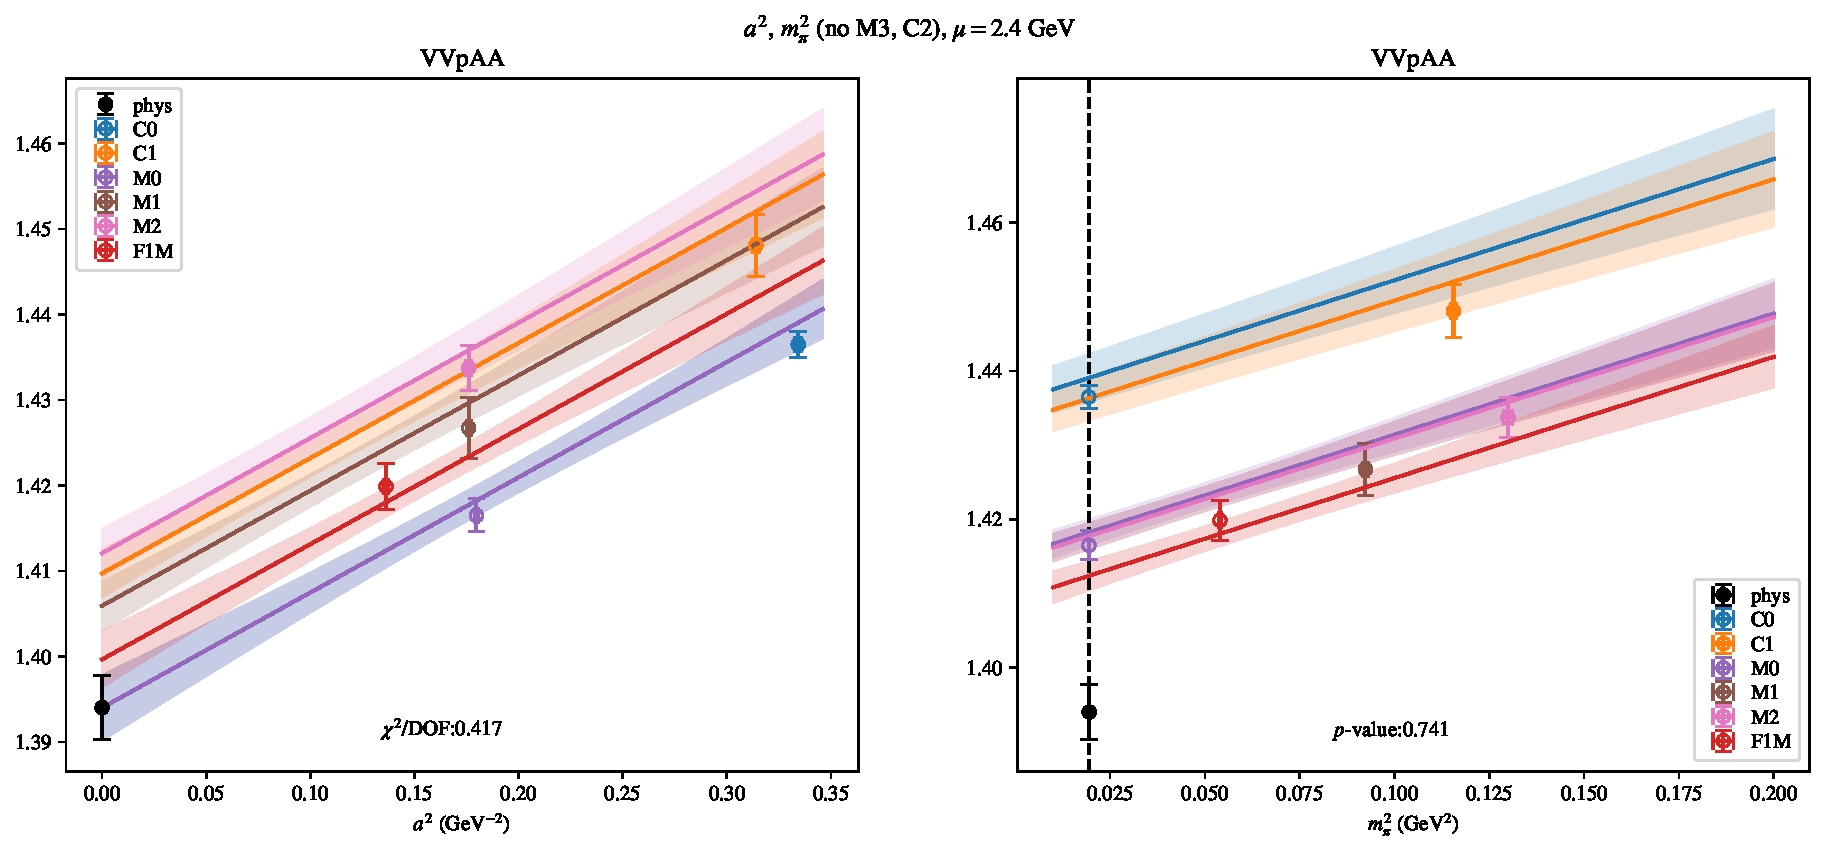
\includepdf[link, pages=-]{VVpAA/SUSY/a2m2mcut_24.pdf}
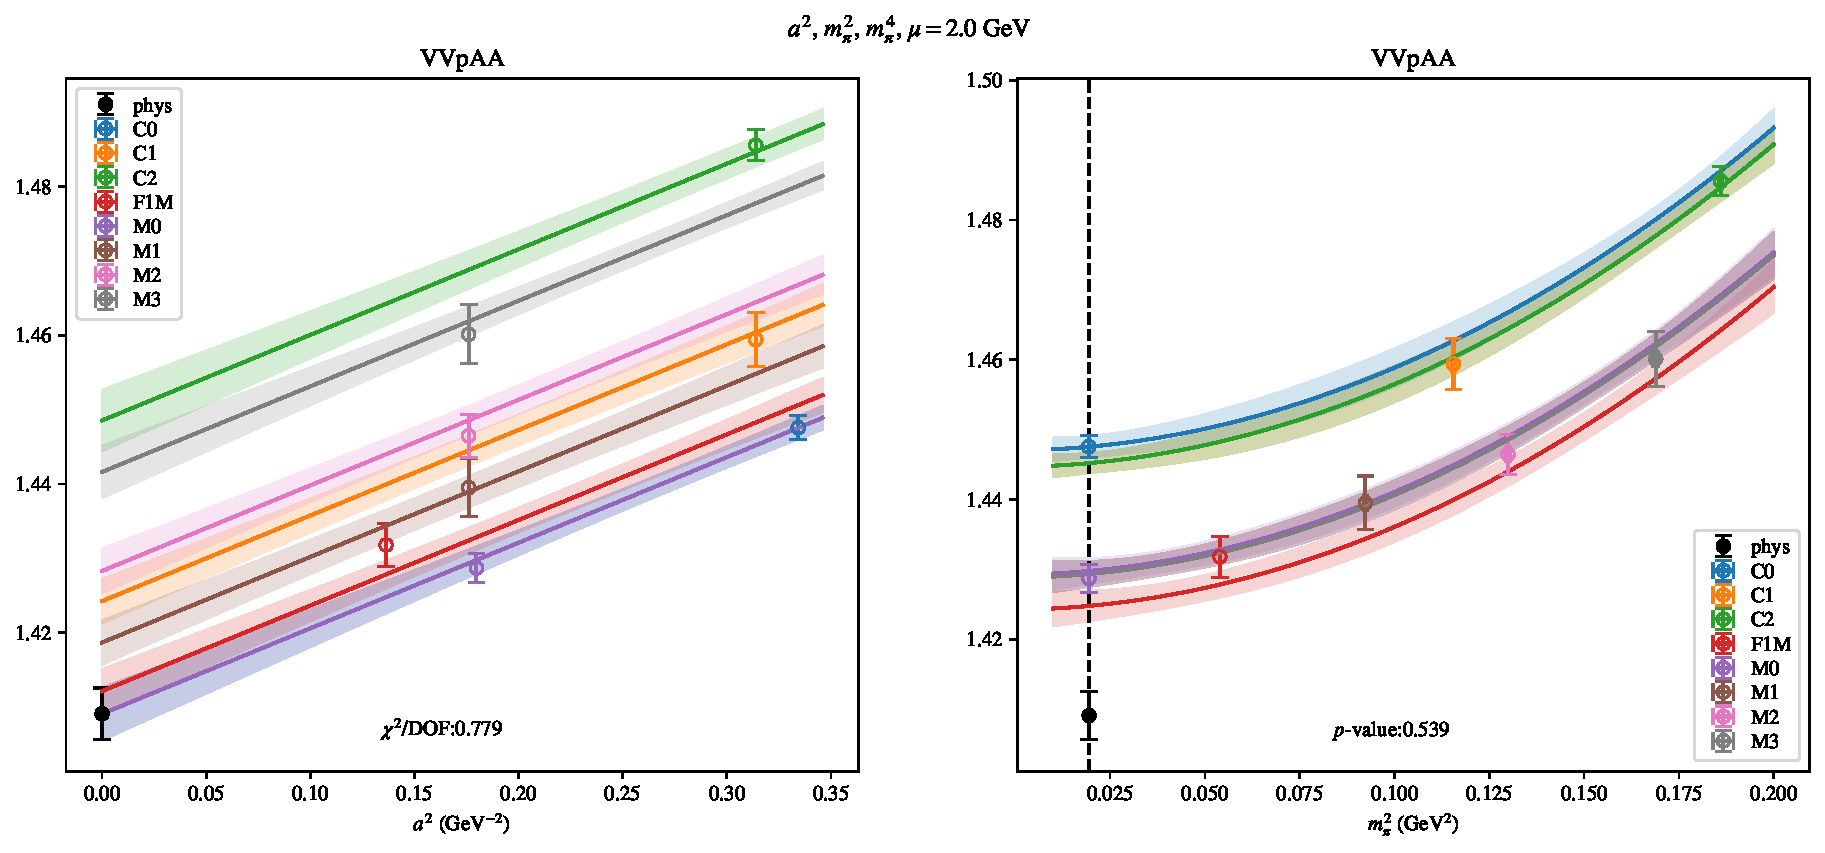
\includepdf[link, pages=-]{VVpAA/SUSY/a2m2m4_20.pdf}
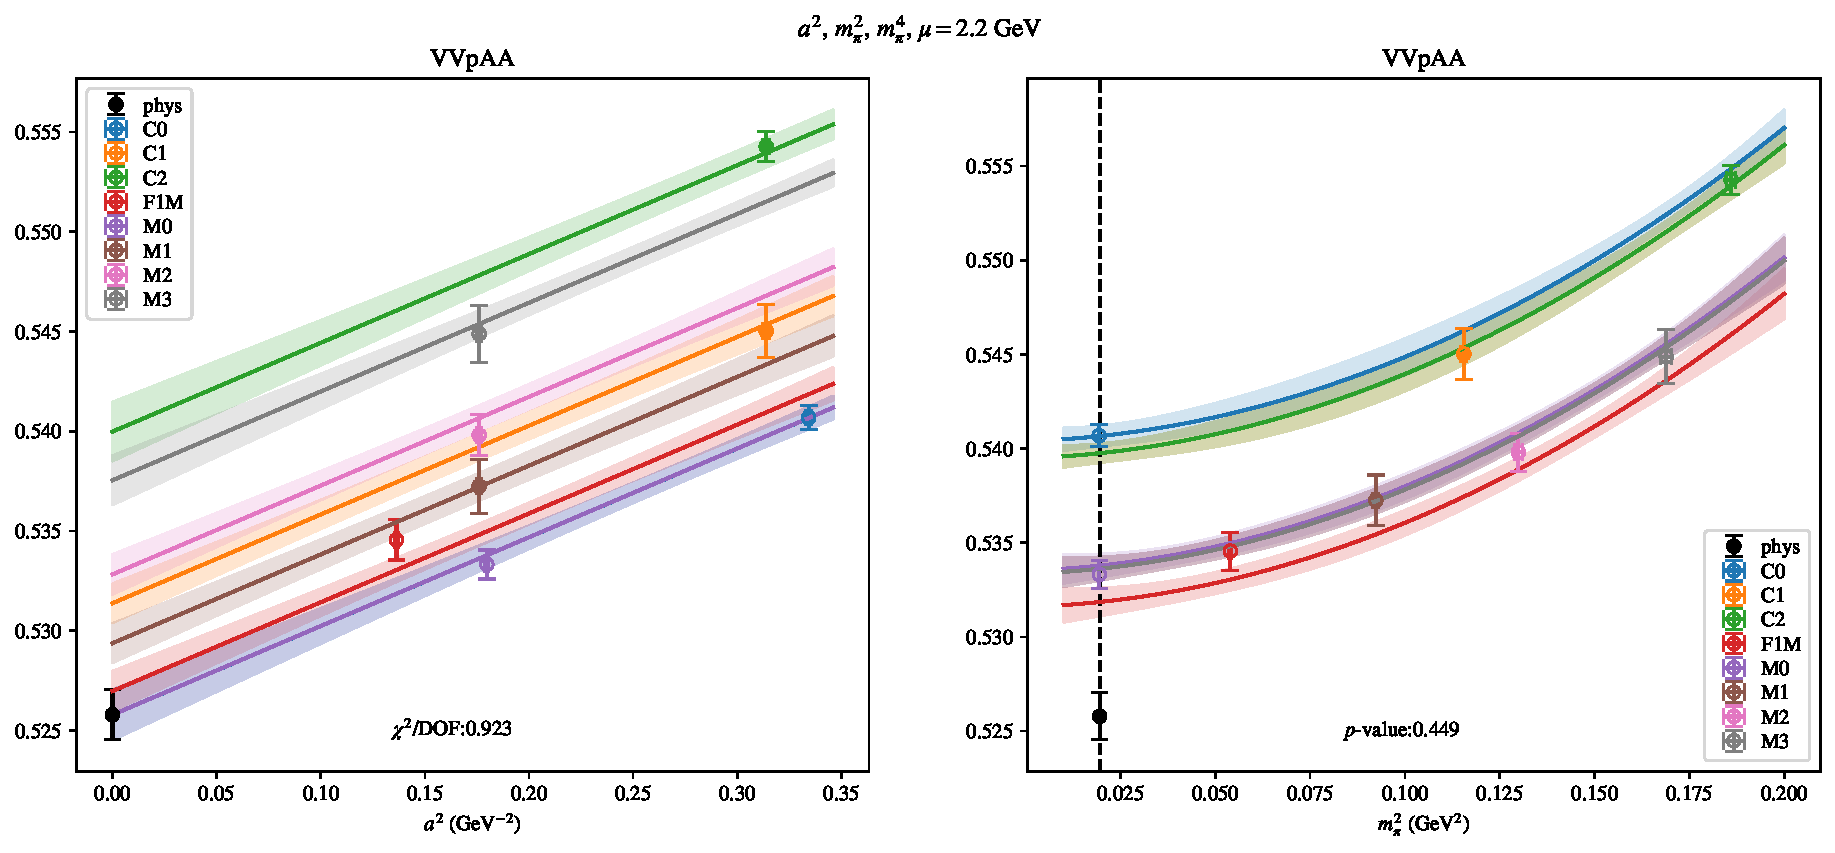
\includepdf[link, pages=-]{VVpAA/SUSY/a2m2m4_22.pdf}
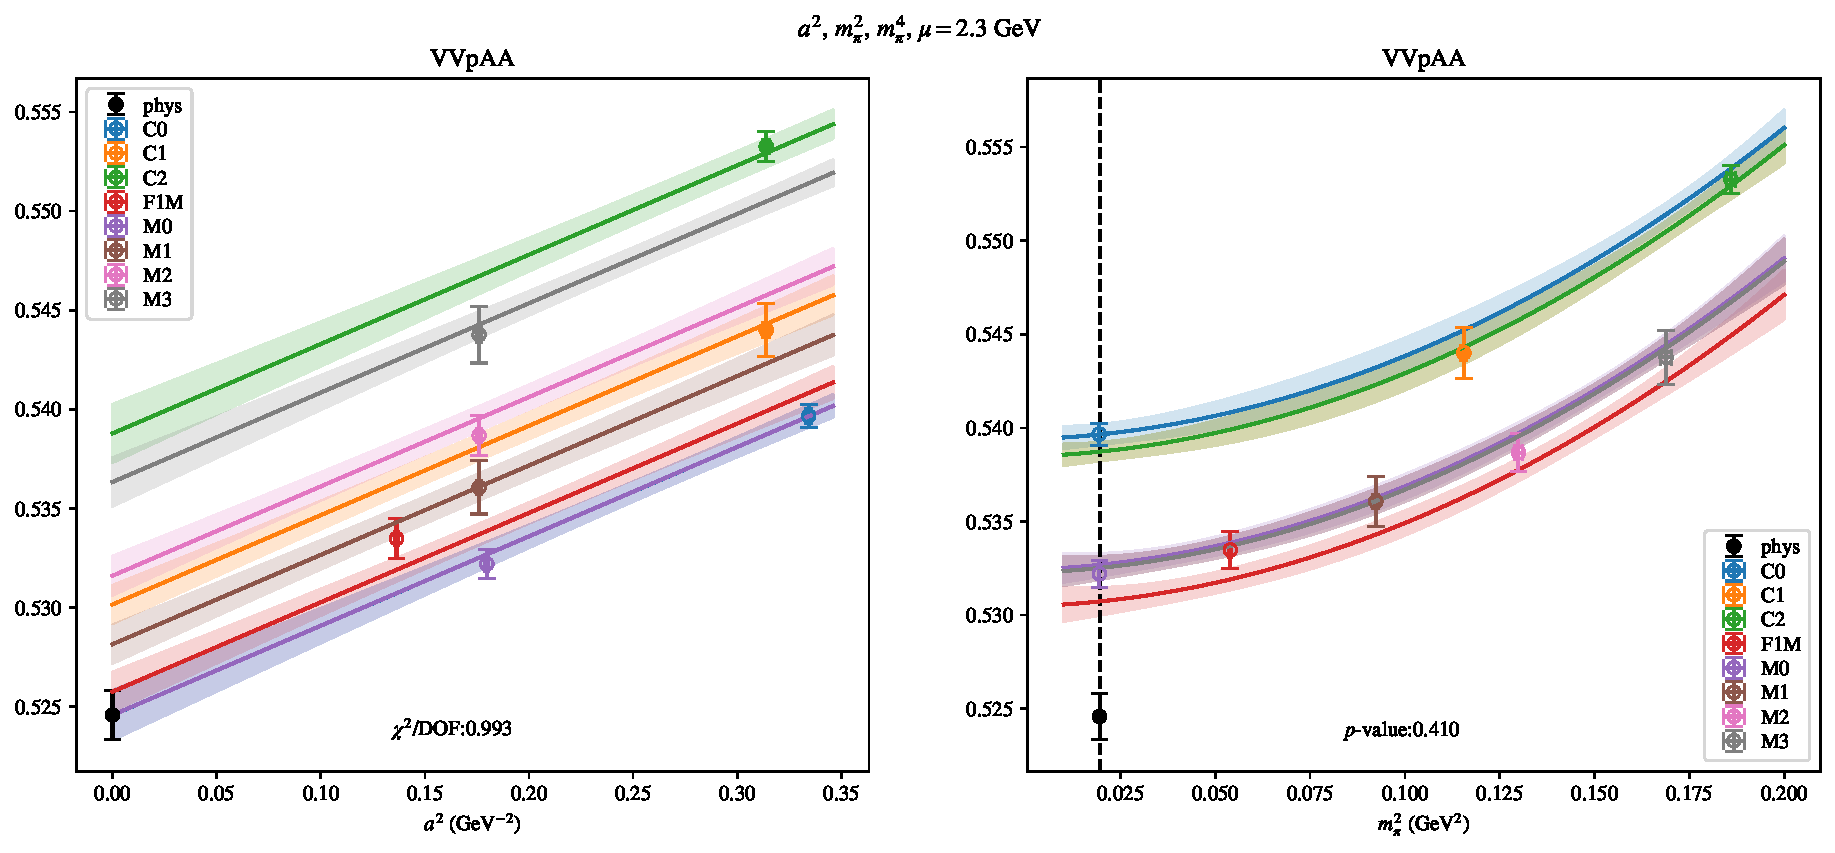
\includepdf[link, pages=-]{VVpAA/SUSY/a2m2m4_23.pdf}
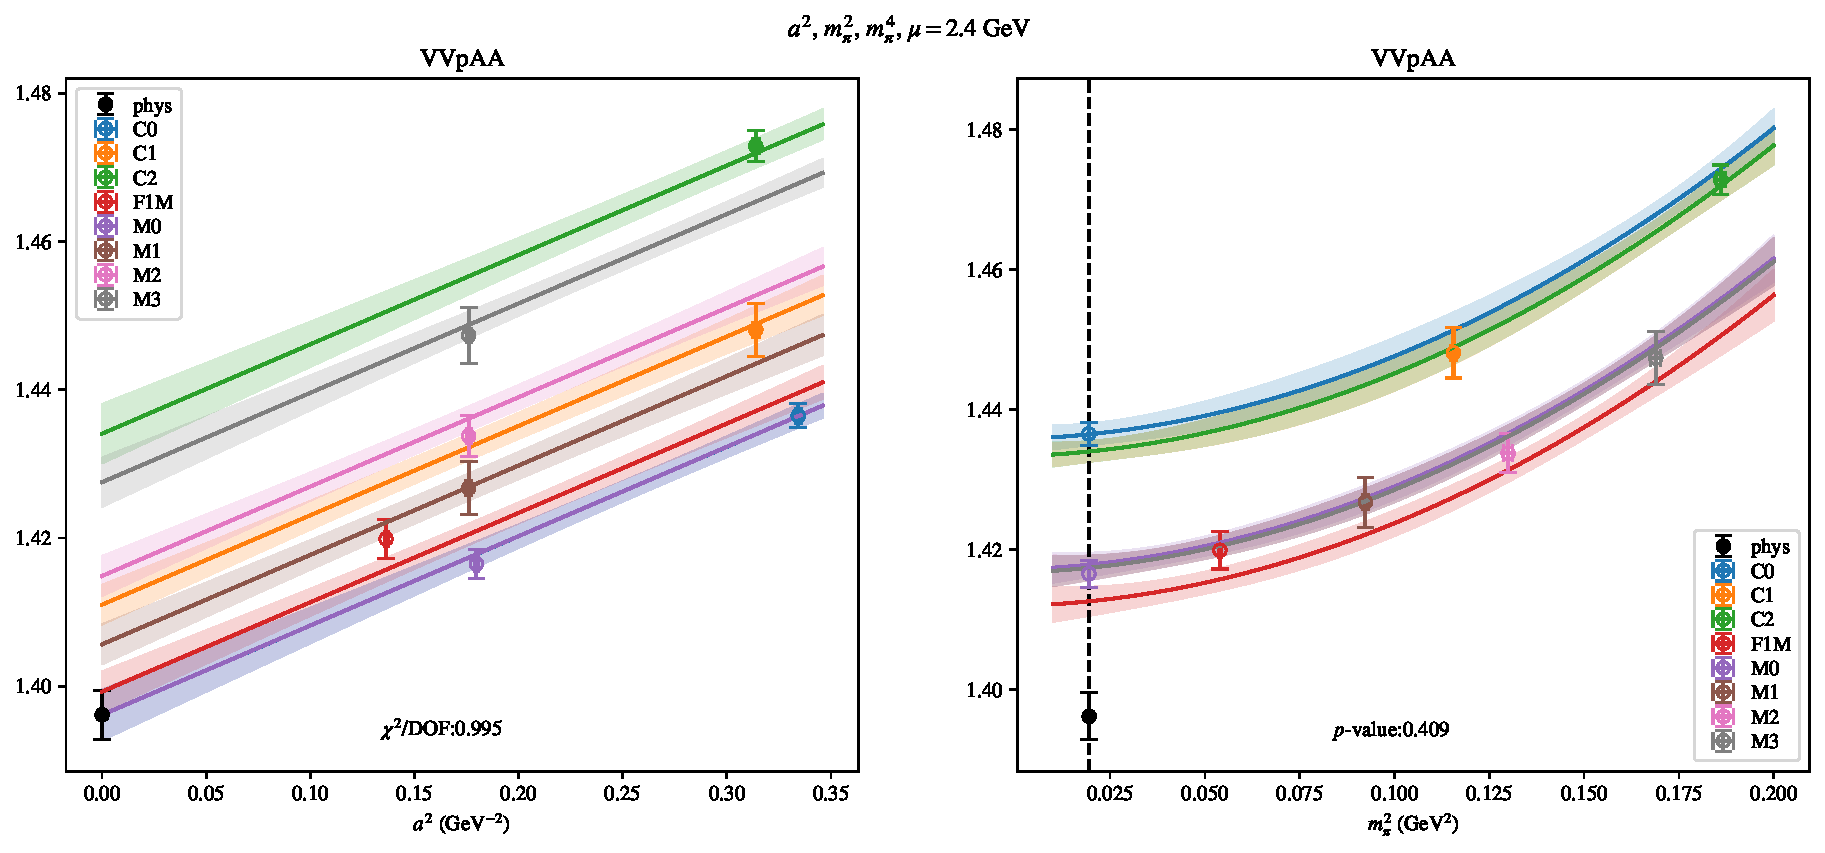
\includepdf[link, pages=-]{VVpAA/SUSY/a2m2m4_24.pdf}
\clearpage
\section{$B_2$}
\begin{table}[h!]
\begin{center}
\begin{tabular}{|c|c|c|c|c|c|}
\hline
$\mu$ (GeV) & $a^2$, $m_\pi^2$& $a^2$, $m_\pi^2$ (no C)& $a^2$, $a^4$, $m_\pi^2$& $a^2$, $m_\pi^2$ (no M3, C2)& $a^2$, $m_\pi^2$, $m_\pi^4$\\
\hline
2.0& \hyperlink{VVmAA/SUSY/a2m2_20.pdf.1}{\textbf{-0.945(15)}: 5.15 (0.0)} & \hyperlink{VVmAA/SUSY/a2m2noC_20.pdf.1}{\textbf{-0.986(92)}: 1.081 (0.339)} & \hyperlink{VVmAA/SUSY/a2a4m2_20.pdf.1}{\textbf{-0.99(14)}: 3.825 (0.004)} & \hyperlink{VVmAA/SUSY/a2m2mcut_20.pdf.1}{\textbf{-0.945(16)}: 7.22 (0.0)} & \hyperlink{VVmAA/SUSY/a2m2m4_20.pdf.1}{\textbf{-0.943(16)}: 4.754 (0.001)}\\
2.2& \hyperlink{VVmAA/SUSY/a2m2_22.pdf.1}{\textbf{-0.918(15)}: 5.8 (0.0)} & \hyperlink{VVmAA/SUSY/a2m2noC_22.pdf.1}{\textbf{-0.956(89)}: 1.541 (0.214)} & \hyperlink{VVmAA/SUSY/a2a4m2_22.pdf.1}{\textbf{-0.95(14)}: 5.661 (0.0)} & \hyperlink{VVmAA/SUSY/a2m2mcut_22.pdf.1}{\textbf{-0.918(16)}: 7.005 (0.0)} & \hyperlink{VVmAA/SUSY/a2m2m4_22.pdf.1}{\textbf{-0.916(16)}: 5.195 (0.0)}\\
2.3& \hyperlink{VVmAA/SUSY/a2m2_23.pdf.1}{\textbf{-0.906(15)}: 5.714 (0.0)} & \hyperlink{VVmAA/SUSY/a2m2noC_23.pdf.1}{\textbf{-0.943(88)}: 1.617 (0.198)} & \hyperlink{VVmAA/SUSY/a2a4m2_23.pdf.1}{\textbf{-0.94(14)}: 5.486 (0.0)} & \hyperlink{VVmAA/SUSY/a2m2mcut_23.pdf.1}{\textbf{-0.906(16)}: 7.078 (0.0)} & \hyperlink{VVmAA/SUSY/a2m2m4_23.pdf.1}{\textbf{-0.904(16)}: 5.265 (0.0)}\\
2.4& \hyperlink{VVmAA/SUSY/a2m2_24.pdf.1}{\textbf{-0.897(15)}: 5.741 (0.0)} & \hyperlink{VVmAA/SUSY/a2m2noC_24.pdf.1}{\textbf{-0.930(87)}: 1.523 (0.218)} & \hyperlink{VVmAA/SUSY/a2a4m2_24.pdf.1}{\textbf{-0.92(14)}: 6.089 (0.0)} & \hyperlink{VVmAA/SUSY/a2m2mcut_24.pdf.1}{\textbf{-0.897(16)}: 7.191 (0.0)} & \hyperlink{VVmAA/SUSY/a2m2m4_24.pdf.1}{\textbf{-0.895(16)}: 5.755 (0.0)}\\
\hline
\end{tabular}
\caption{Physical point value from chiral and continuum extrapolation at renormalisation scale $\mu$. Entries are \textbf{value(error)}: $\chi^2/\text{DOF}$ ($p$-value).}
\end{center}
\end{table}
\begin{table}[h!]
\begin{center}
\begin{tabular}{|c c|c|c|c|c|c|}
\hline
$\mu$ (GeV) &  & $a^2$, $m_\pi^2$& $a^2$, $m_\pi^2$ (no C)& $a^2$, $a^4$, $m_\pi^2$& $a^2$, $m_\pi^2$ (no M3, C2)& $a^2$, $m_\pi^2$, $m_\pi^4$\\
\hline
\multirow{2}{0.5in}{2.0} & $\alpha$ & 0.3806(69)& 0.133(55)& -0.075& 0.3807(74)& 0.3881(74)\\
 & $\beta$ & 0.00800(18)& 0.00728(27)& 0.00776(18)& 0.00838(28)& 0.01021(73)\\
\hline
\multirow{2}{0.5in}{2.2} & $\alpha$ & 0.4225(75)& 0.184(55)& 0.057& 0.4212(79)& 0.4303(78)\\
 & $\beta$ & 0.00771(15)& 0.00692(24)& 0.00754(16)& 0.00822(28)& 0.01010(76)\\
\hline
\multirow{2}{0.5in}{2.3} & $\alpha$ & 0.4448(76)& 0.206(56)& 0.076& 0.4435(80)& 0.4522(79)\\
 & $\beta$ & 0.00768(15)& 0.00689(24)& 0.00750(16)& 0.00812(27)& 0.00990(75)\\
\hline
\multirow{2}{0.5in}{2.4} & $\alpha$ & 0.4624(76)& 0.245(56)& 0.16(14)& 0.4601(81)& 0.4693(81)\\
 & $\beta$ & 0.00769(14)& 0.00688(22)& 0.00755(15)& 0.00804(25)& 0.00957(72)\\
\hline
\end{tabular}
\caption{Fit values of coefficients in $B = B_{phys} + \mathbf{\alpha} a^2 + \mathbf{\beta}\left(\frac{m_\pi^2}{f_\pi^2}-\frac{m_{\pi,PDG}^2}{f_\pi^2}\right) + \ldots$.}
\end{center}
\end{table}
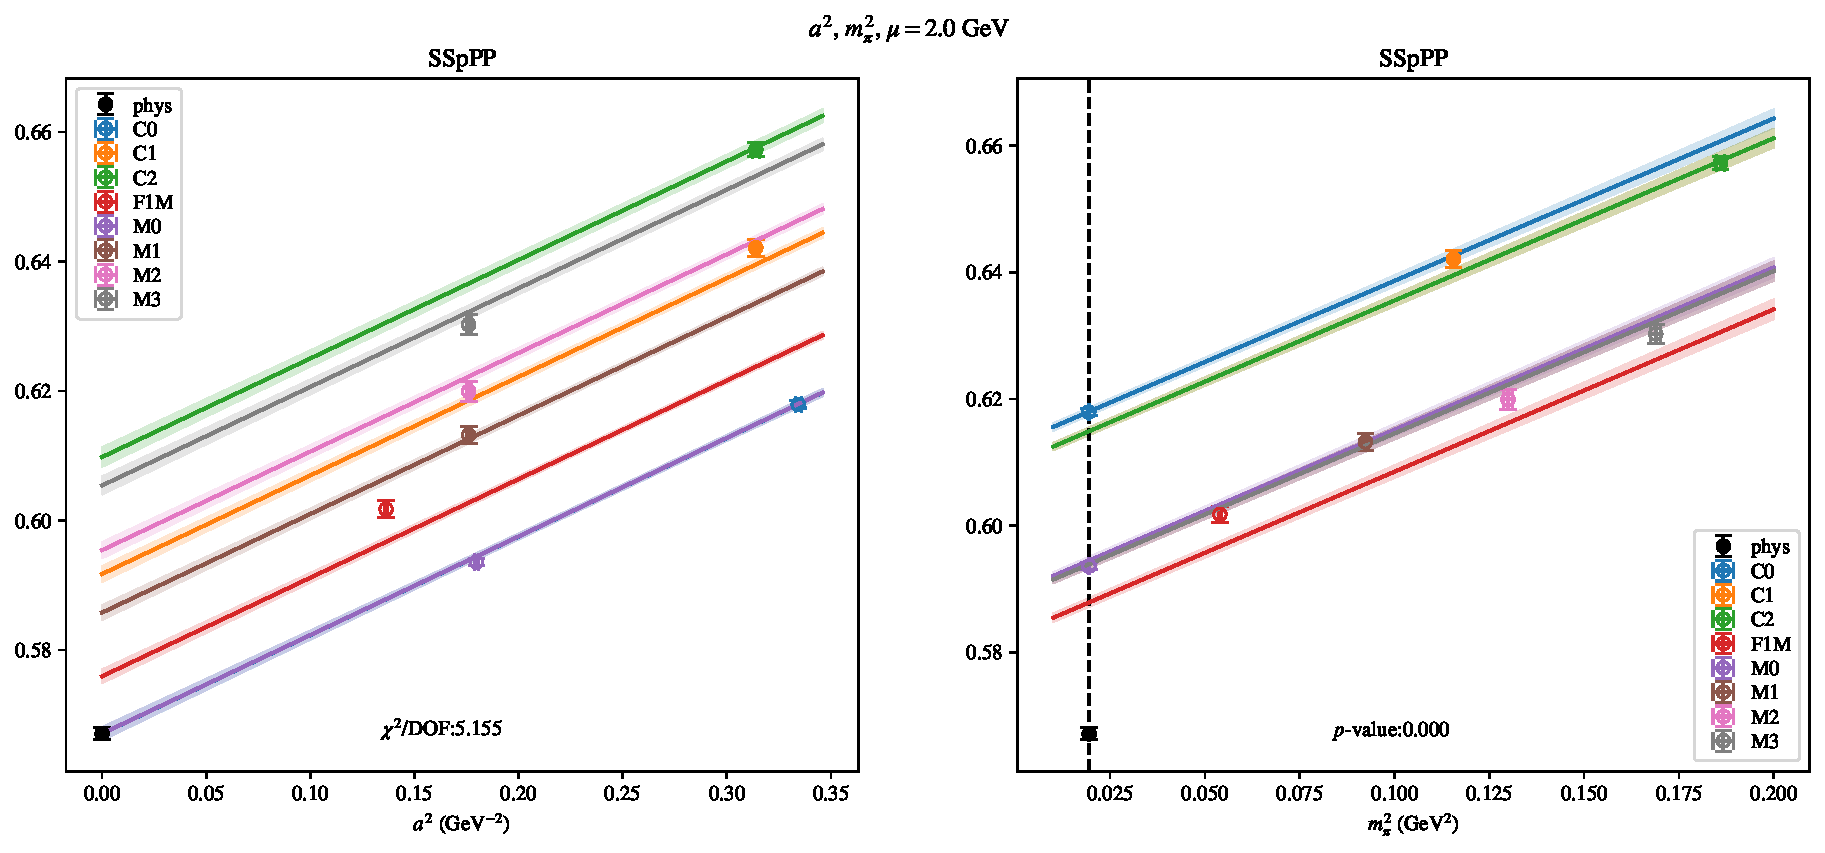
\includepdf[link, pages=-]{VVmAA/SUSY/a2m2_20.pdf}
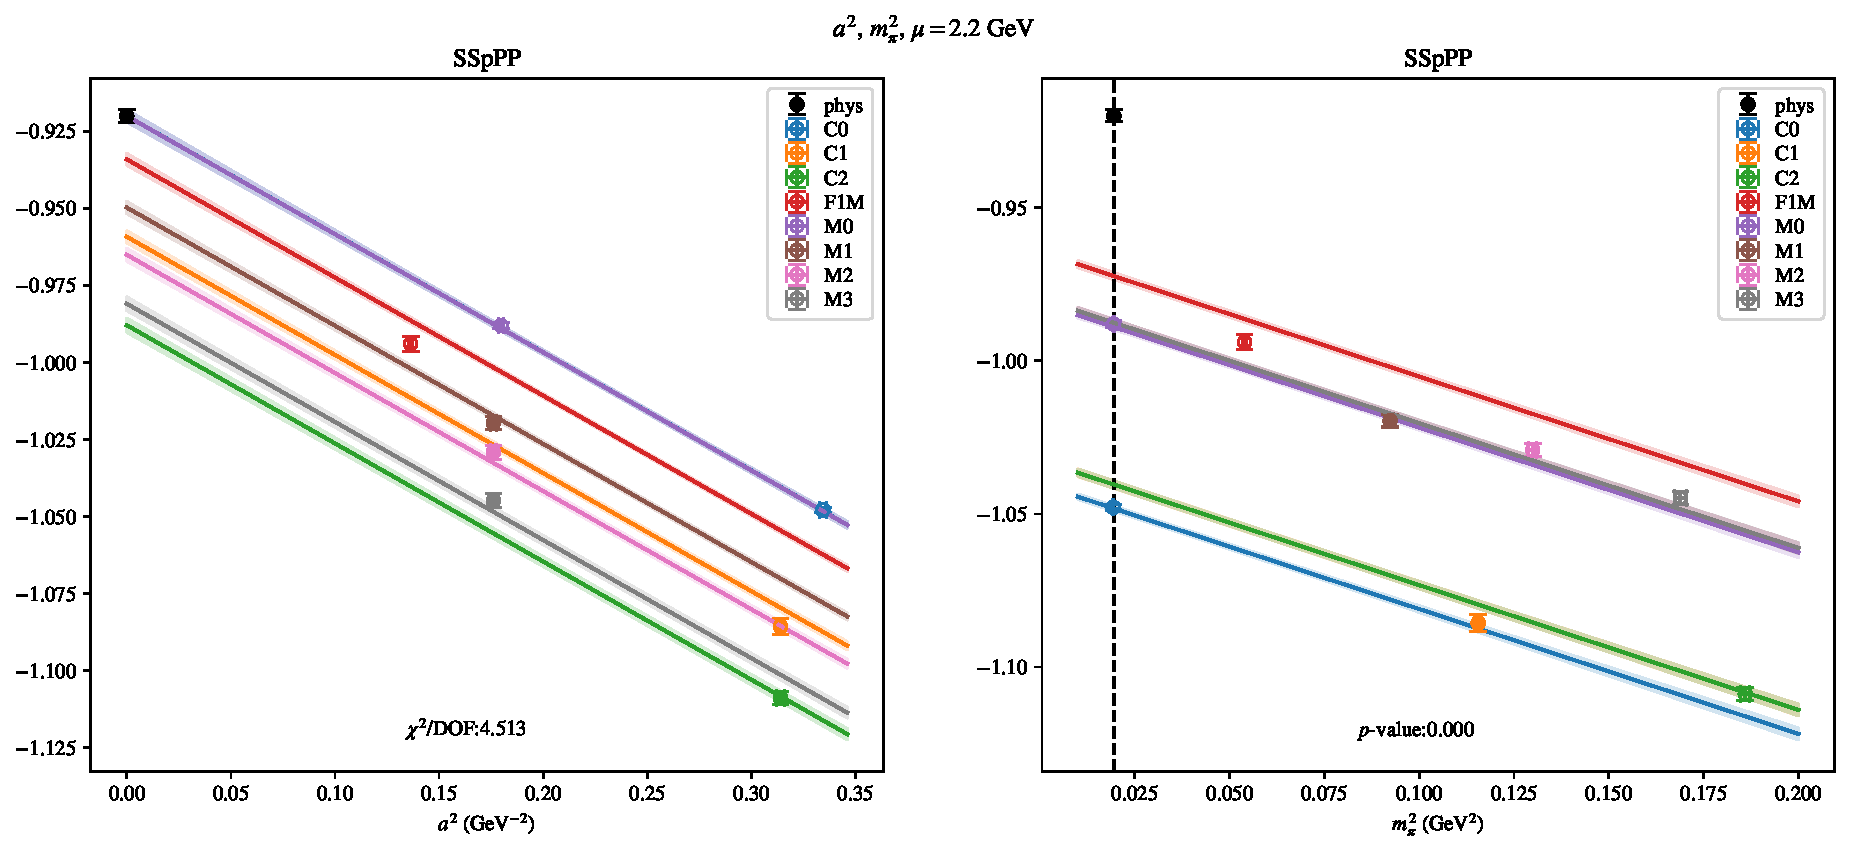
\includepdf[link, pages=-]{VVmAA/SUSY/a2m2_22.pdf}
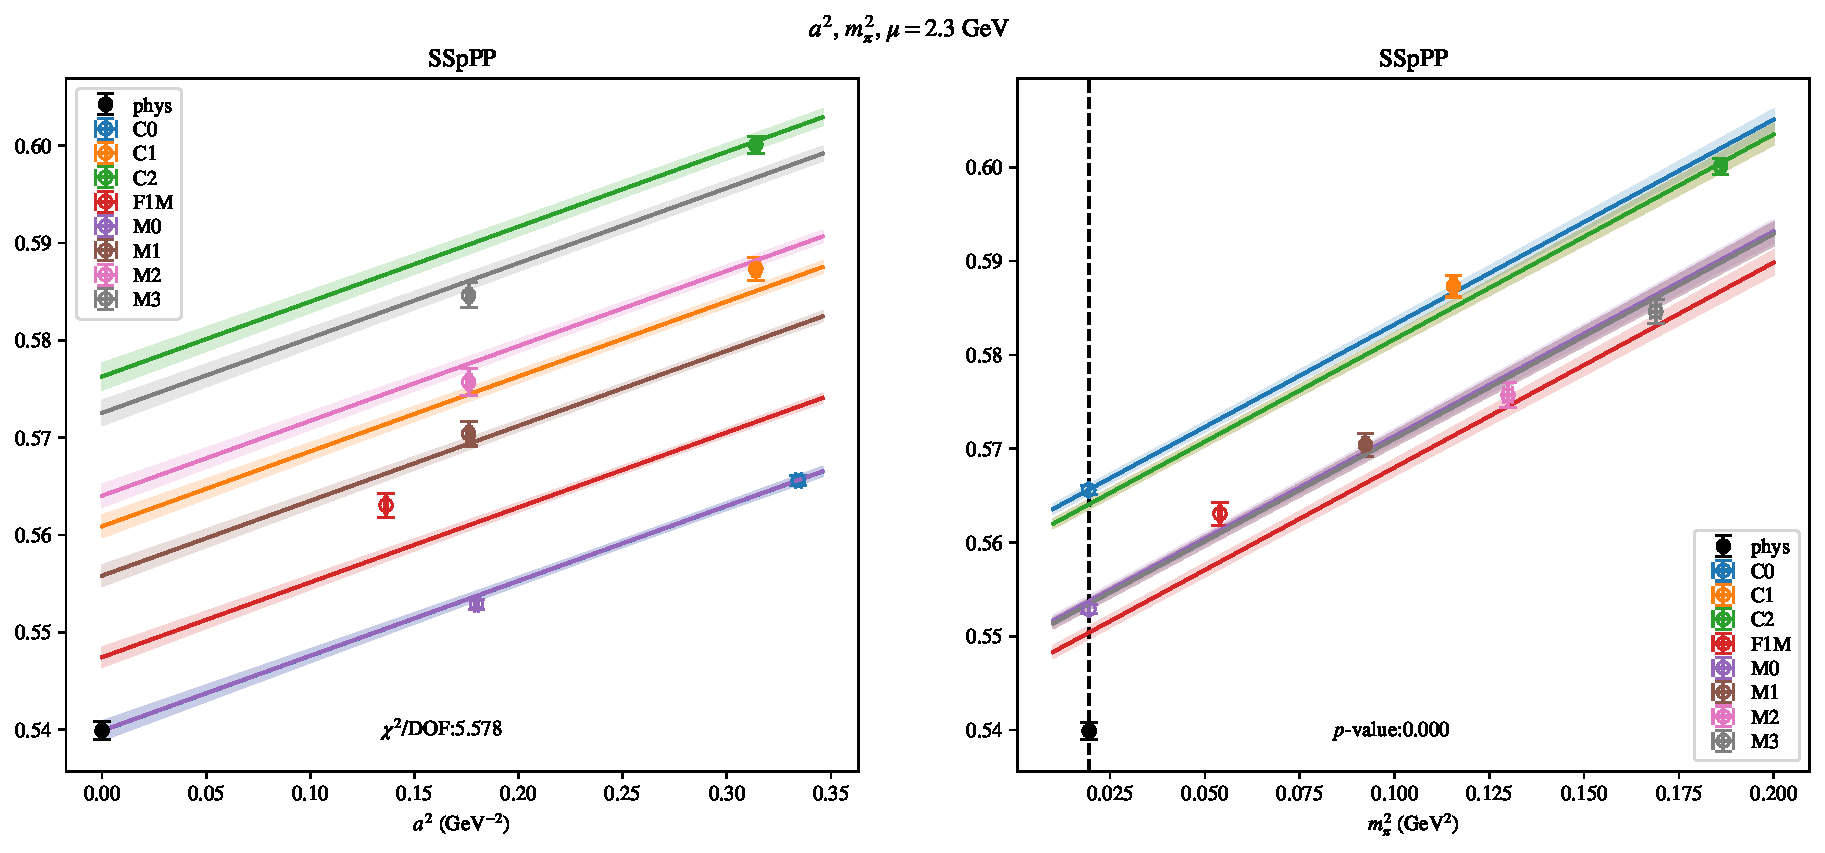
\includepdf[link, pages=-]{VVmAA/SUSY/a2m2_23.pdf}
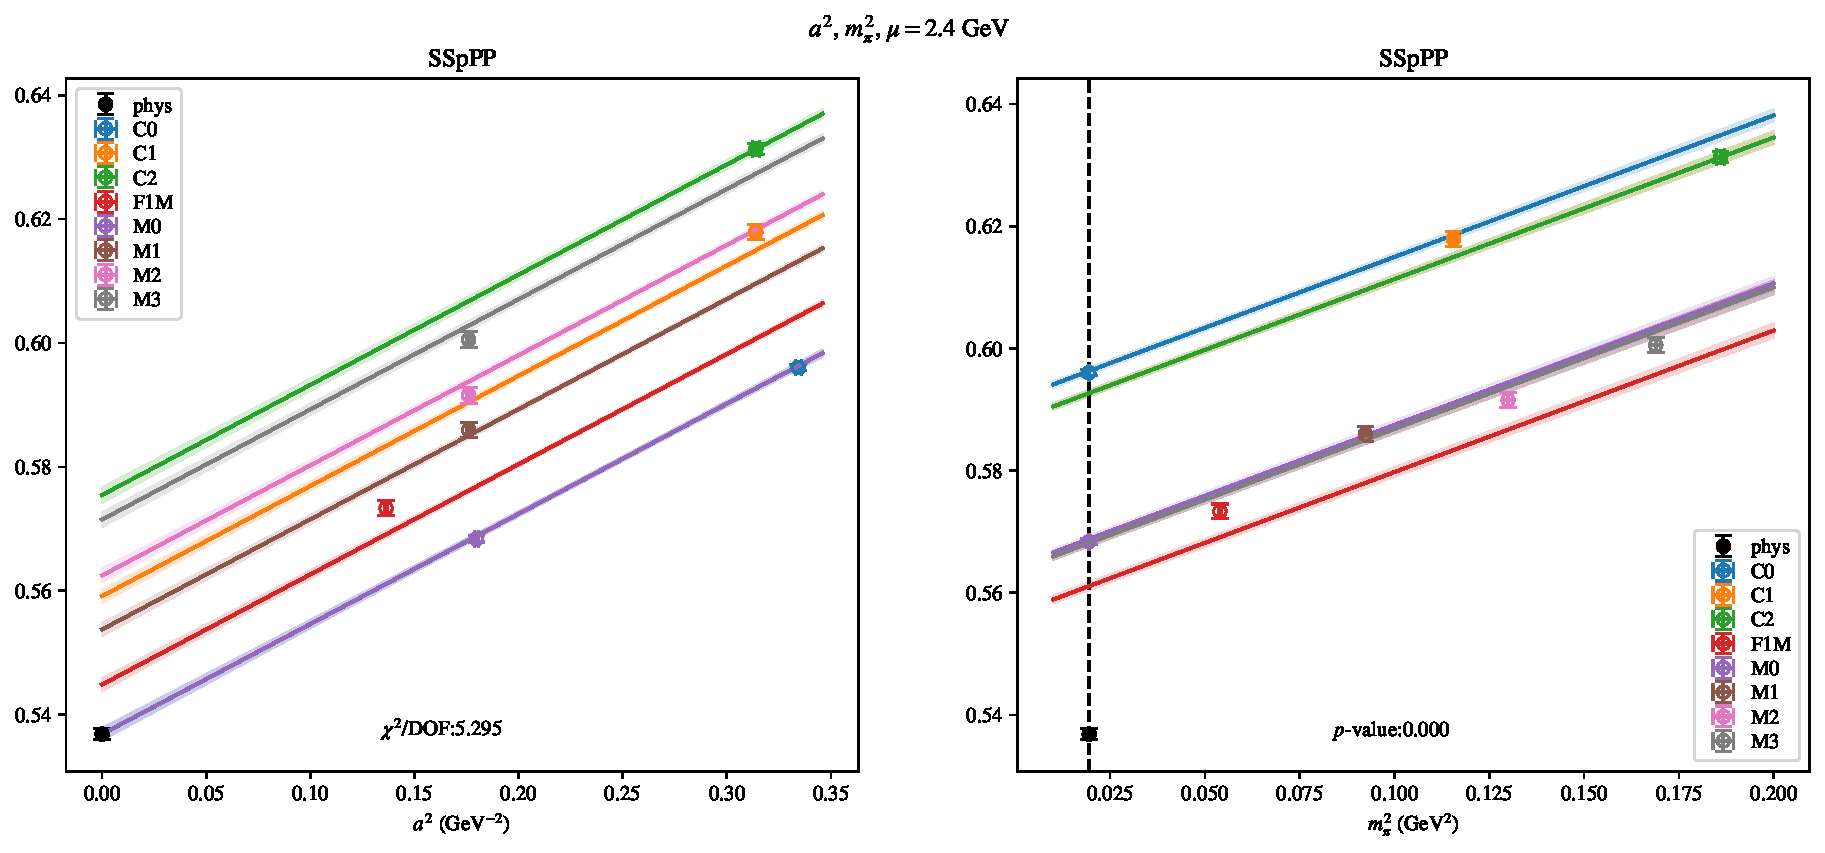
\includepdf[link, pages=-]{VVmAA/SUSY/a2m2_24.pdf}
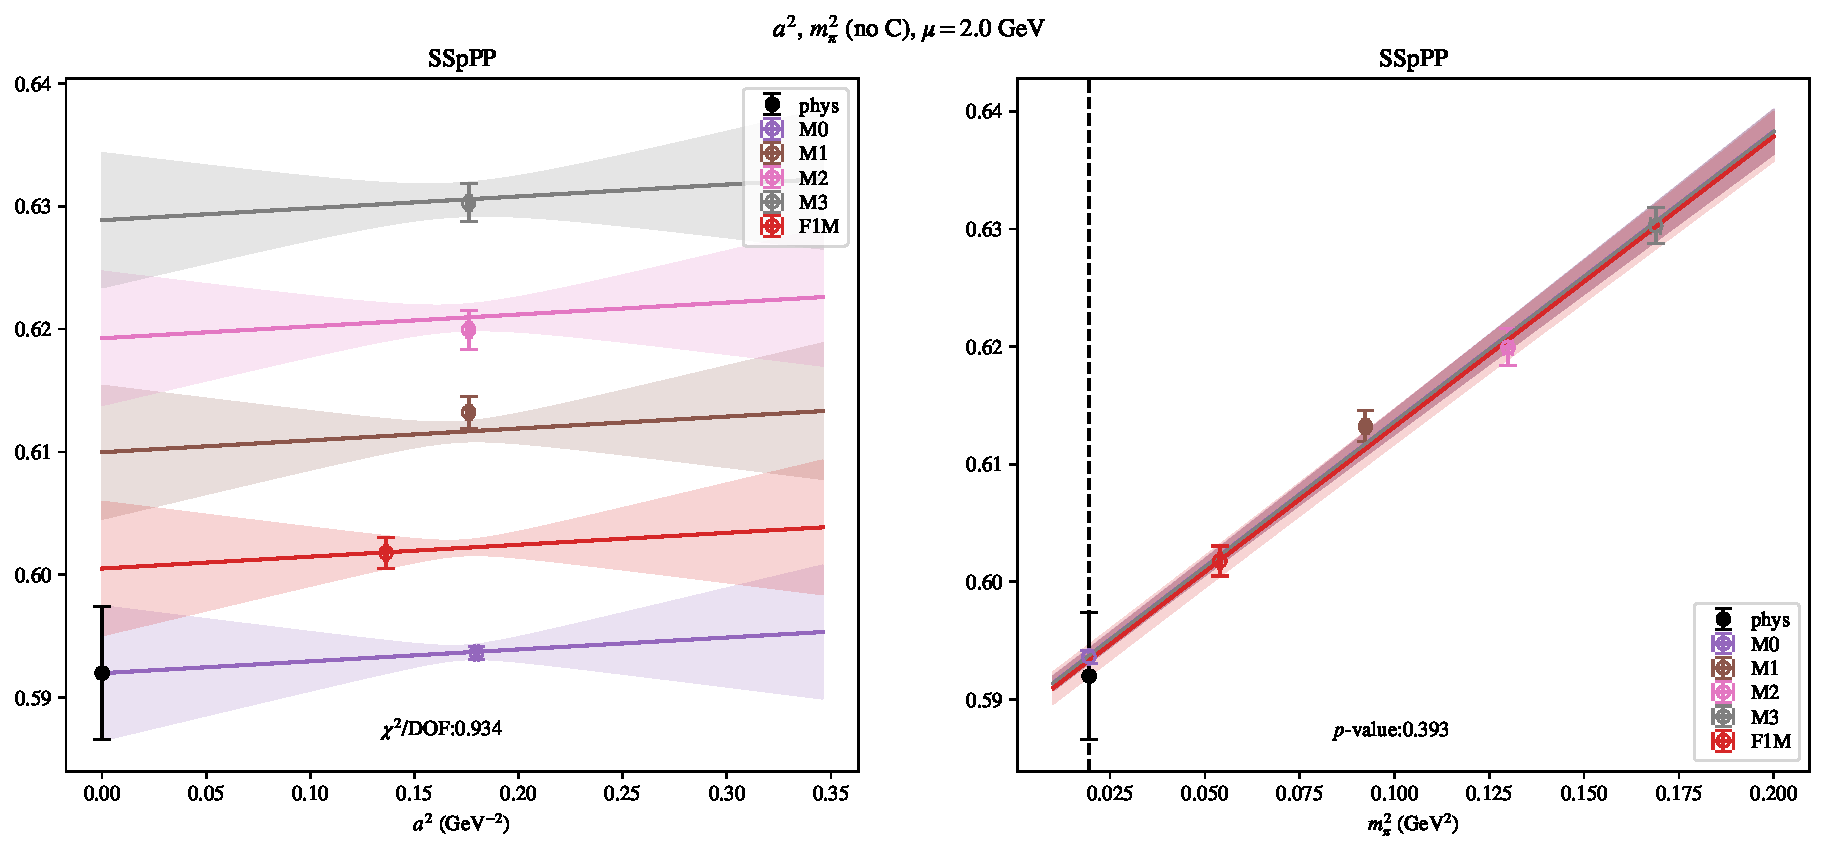
\includepdf[link, pages=-]{VVmAA/SUSY/a2m2noC_20.pdf}
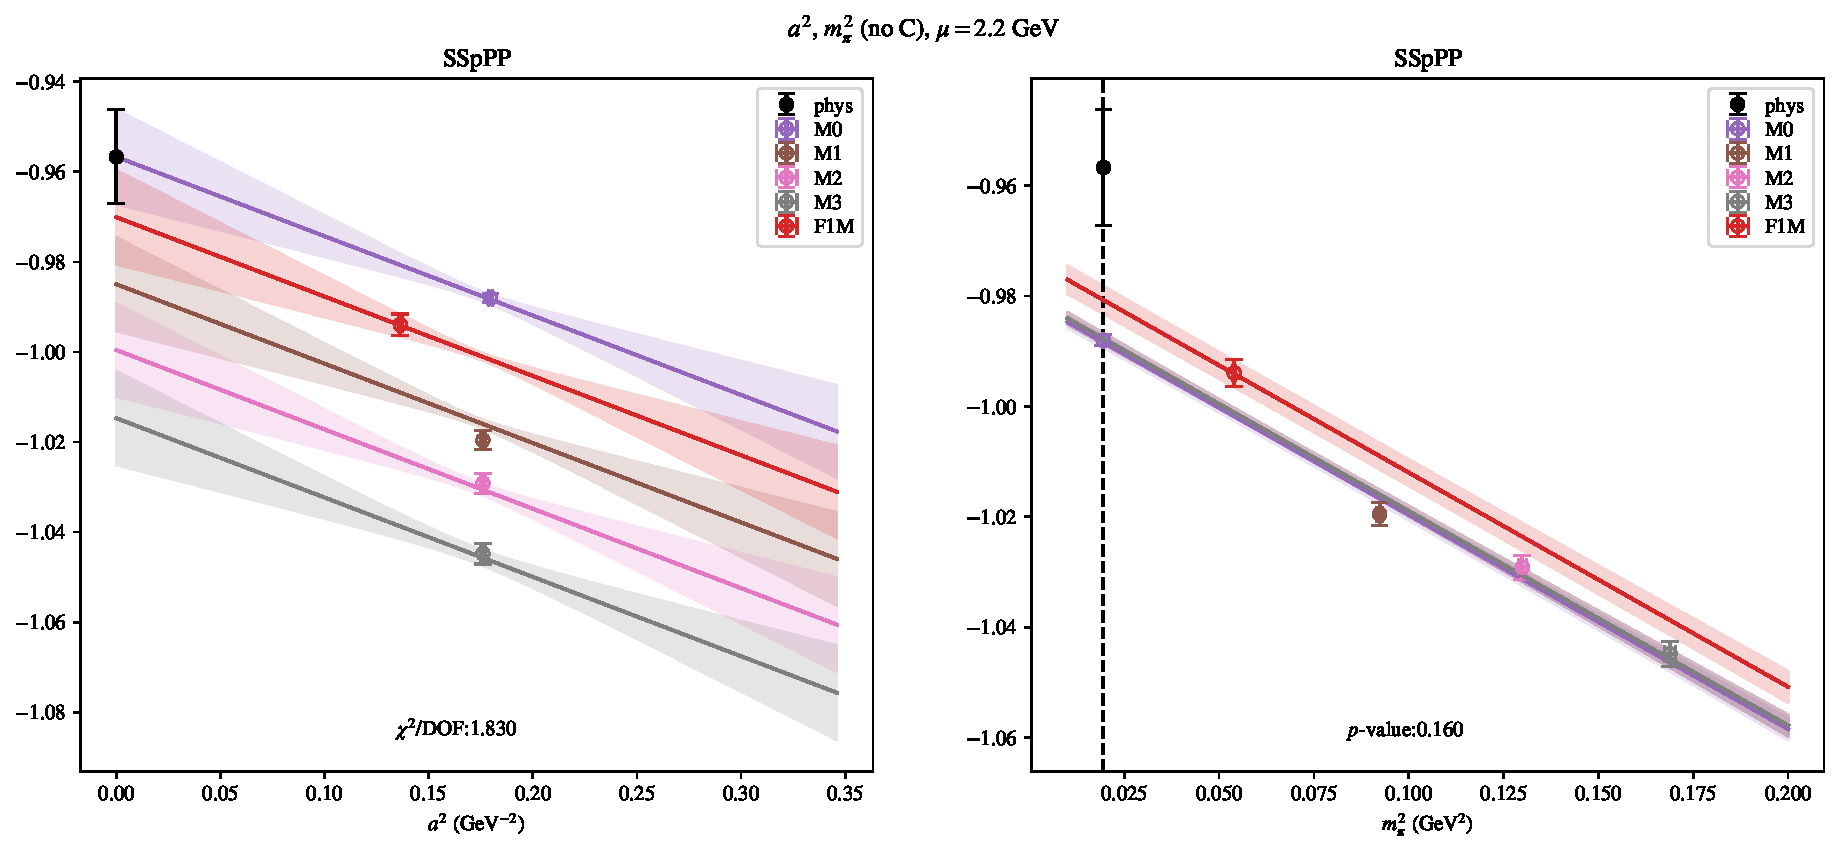
\includepdf[link, pages=-]{VVmAA/SUSY/a2m2noC_22.pdf}
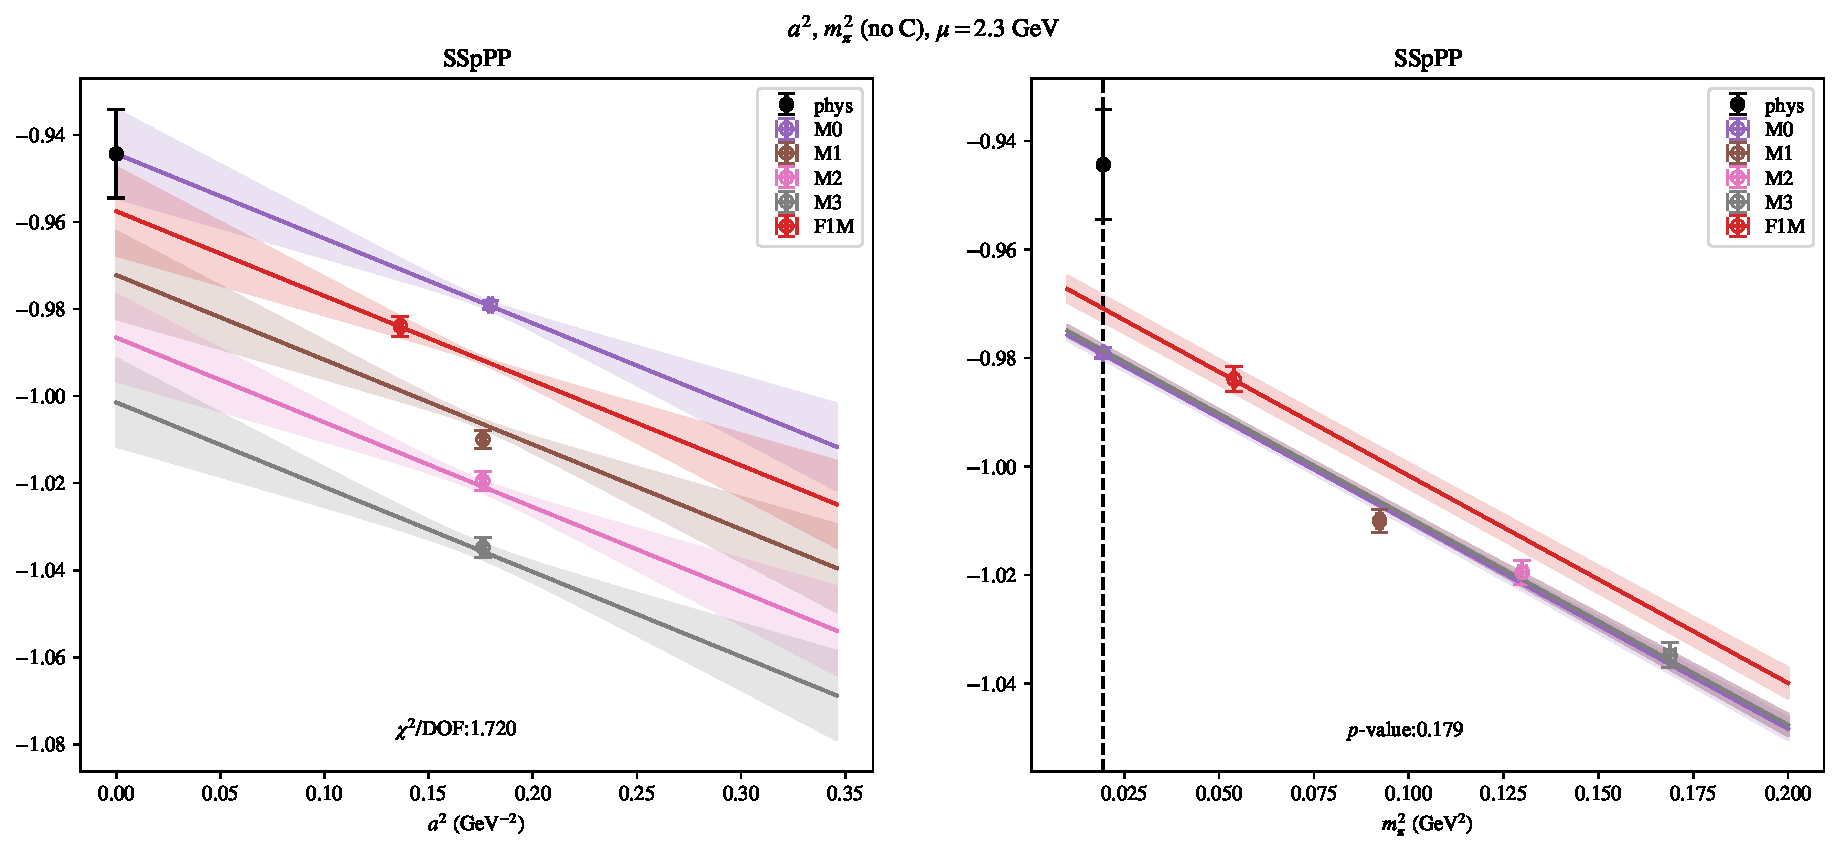
\includepdf[link, pages=-]{VVmAA/SUSY/a2m2noC_23.pdf}
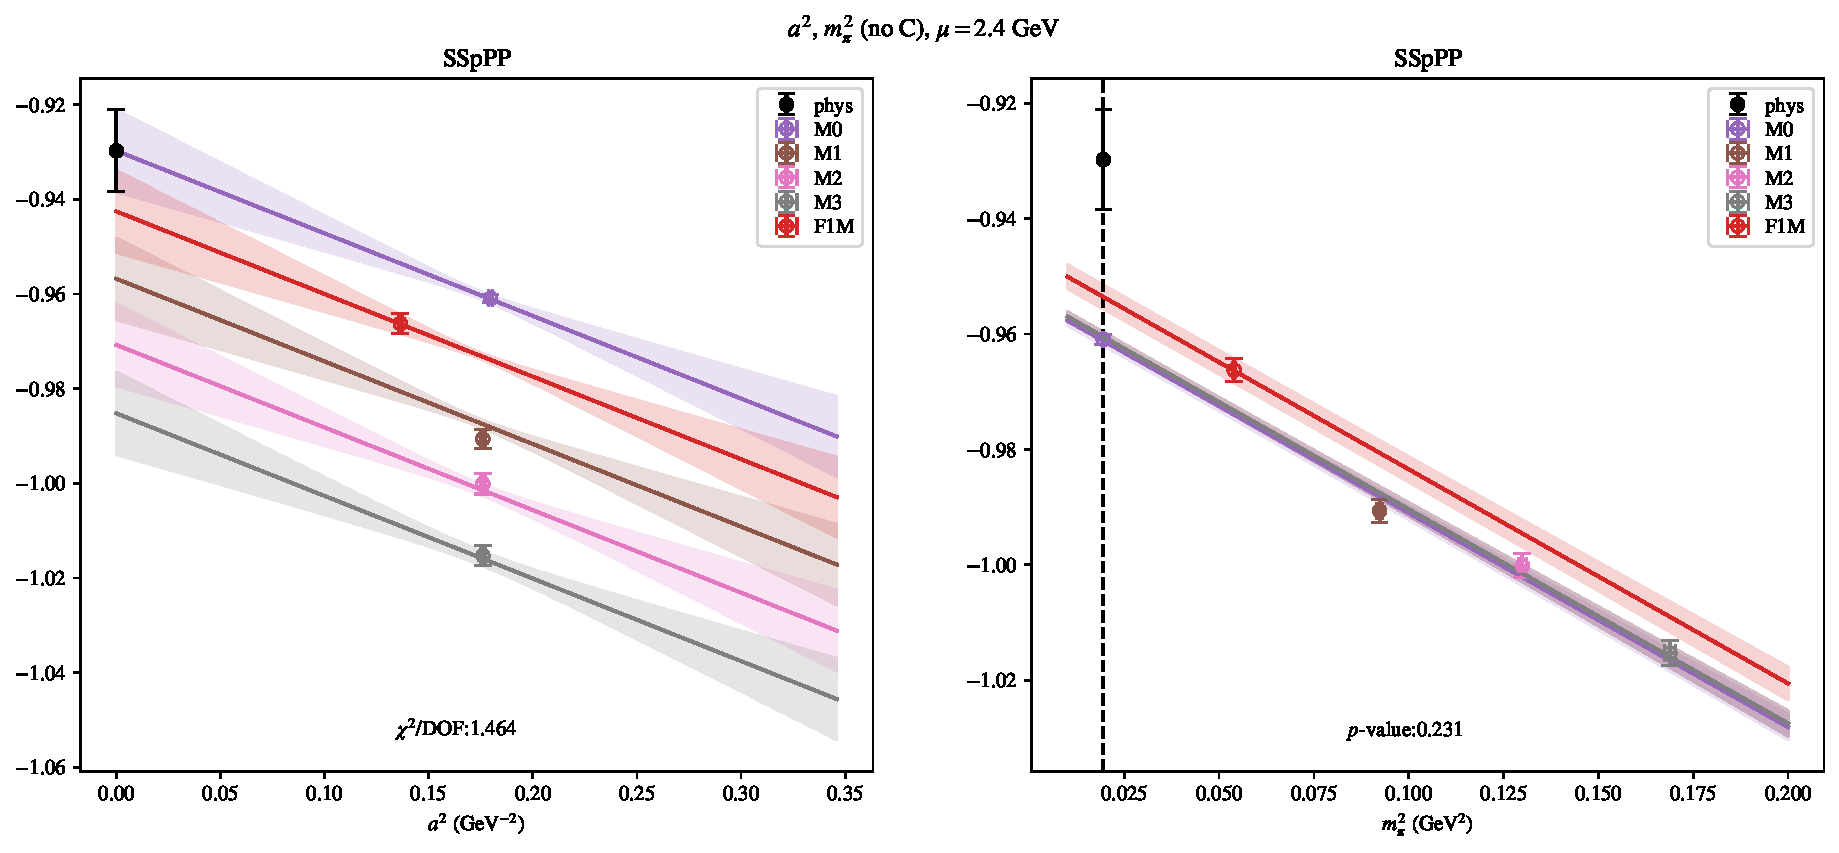
\includepdf[link, pages=-]{VVmAA/SUSY/a2m2noC_24.pdf}
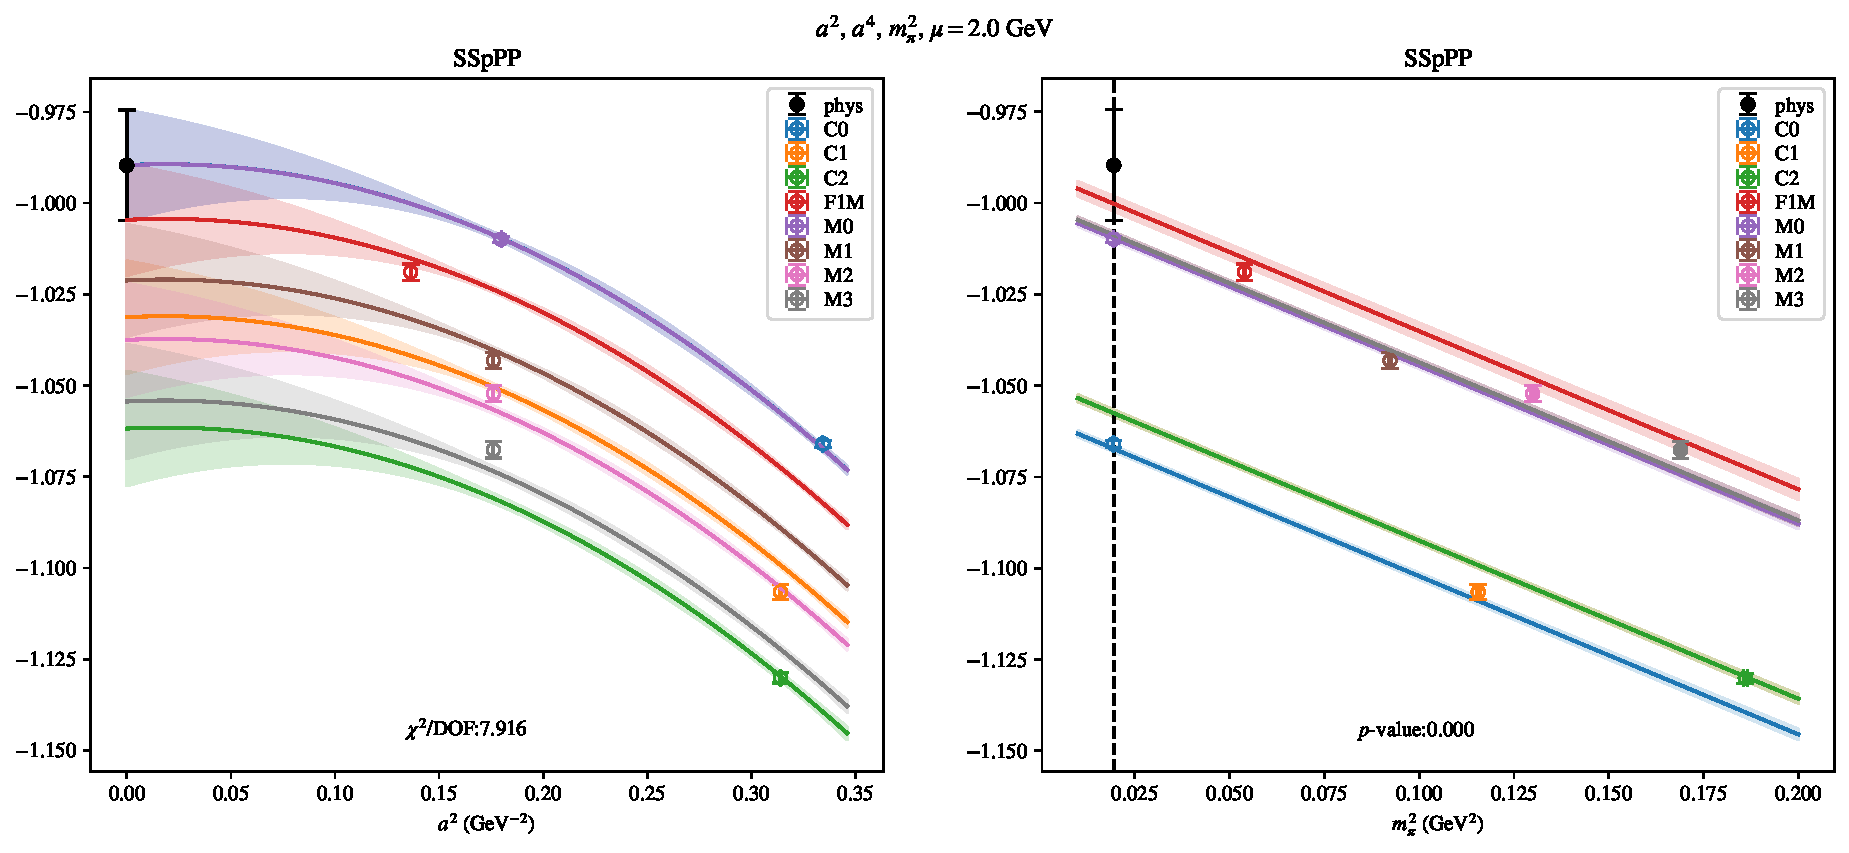
\includepdf[link, pages=-]{VVmAA/SUSY/a2a4m2_20.pdf}
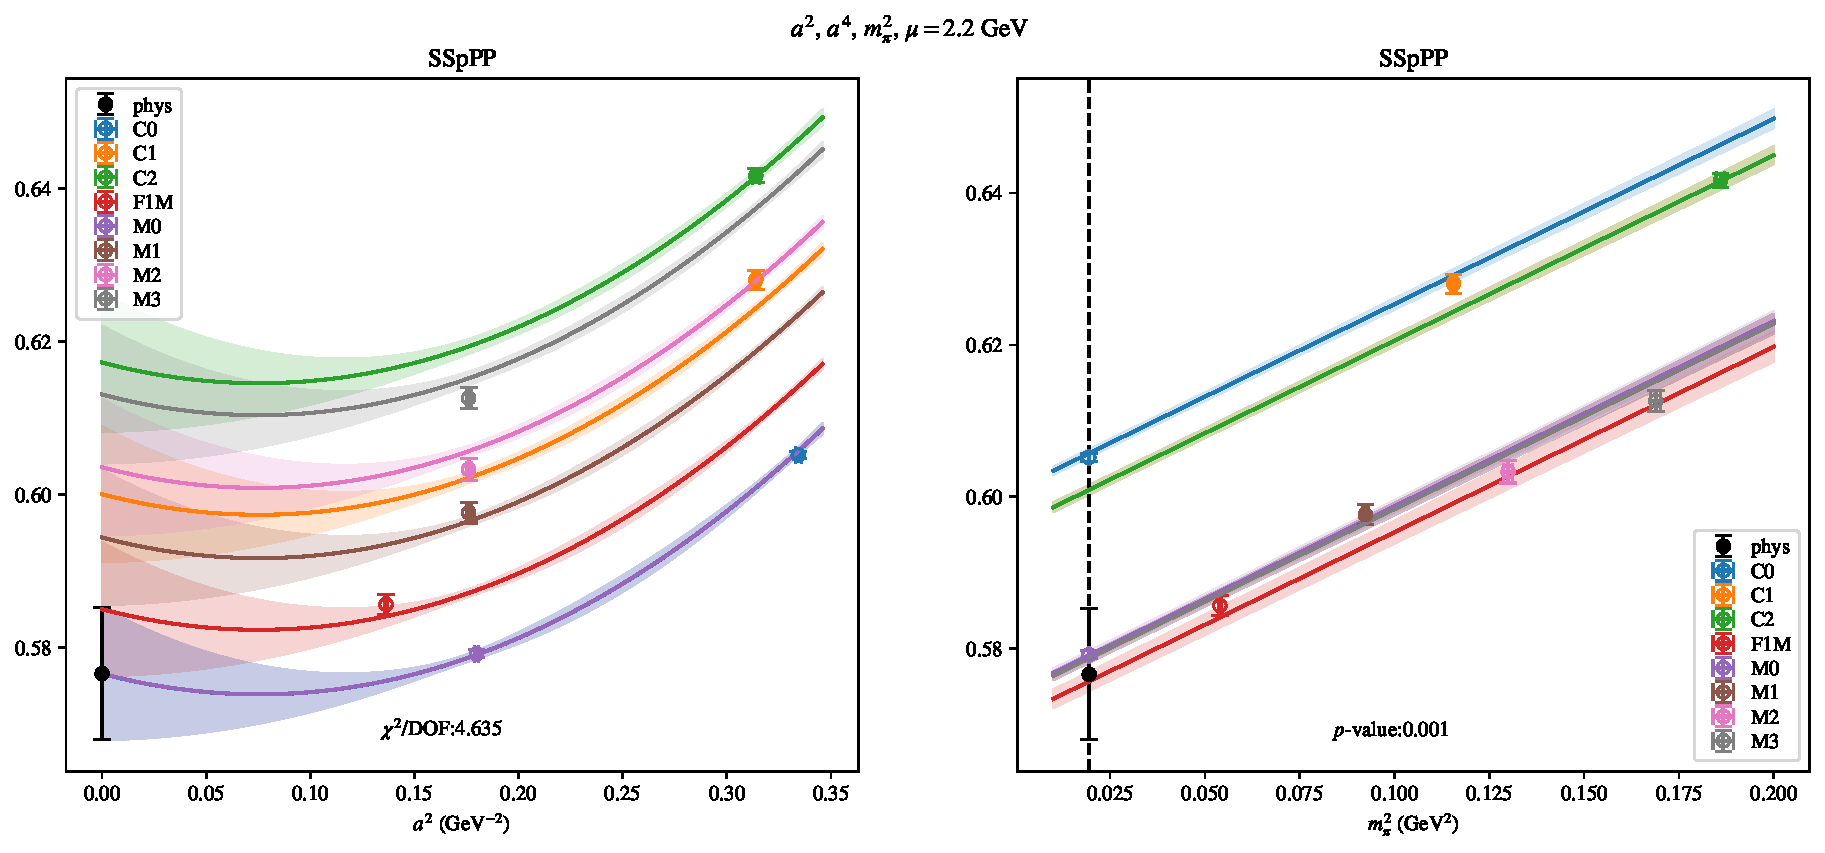
\includepdf[link, pages=-]{VVmAA/SUSY/a2a4m2_22.pdf}
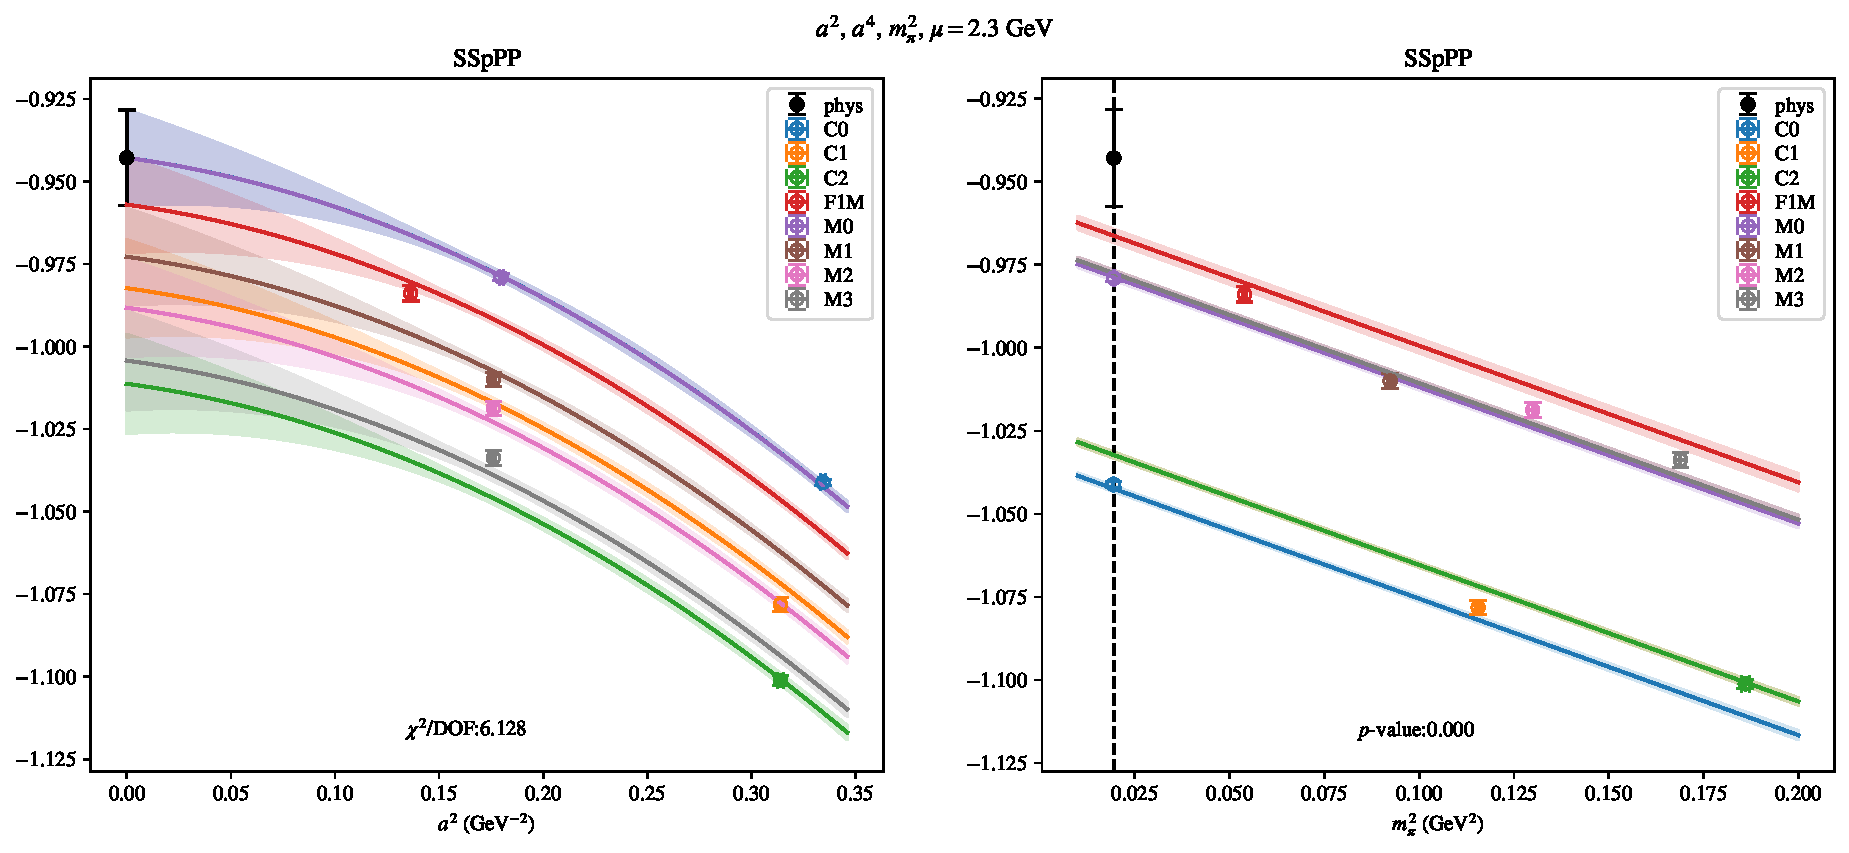
\includepdf[link, pages=-]{VVmAA/SUSY/a2a4m2_23.pdf}
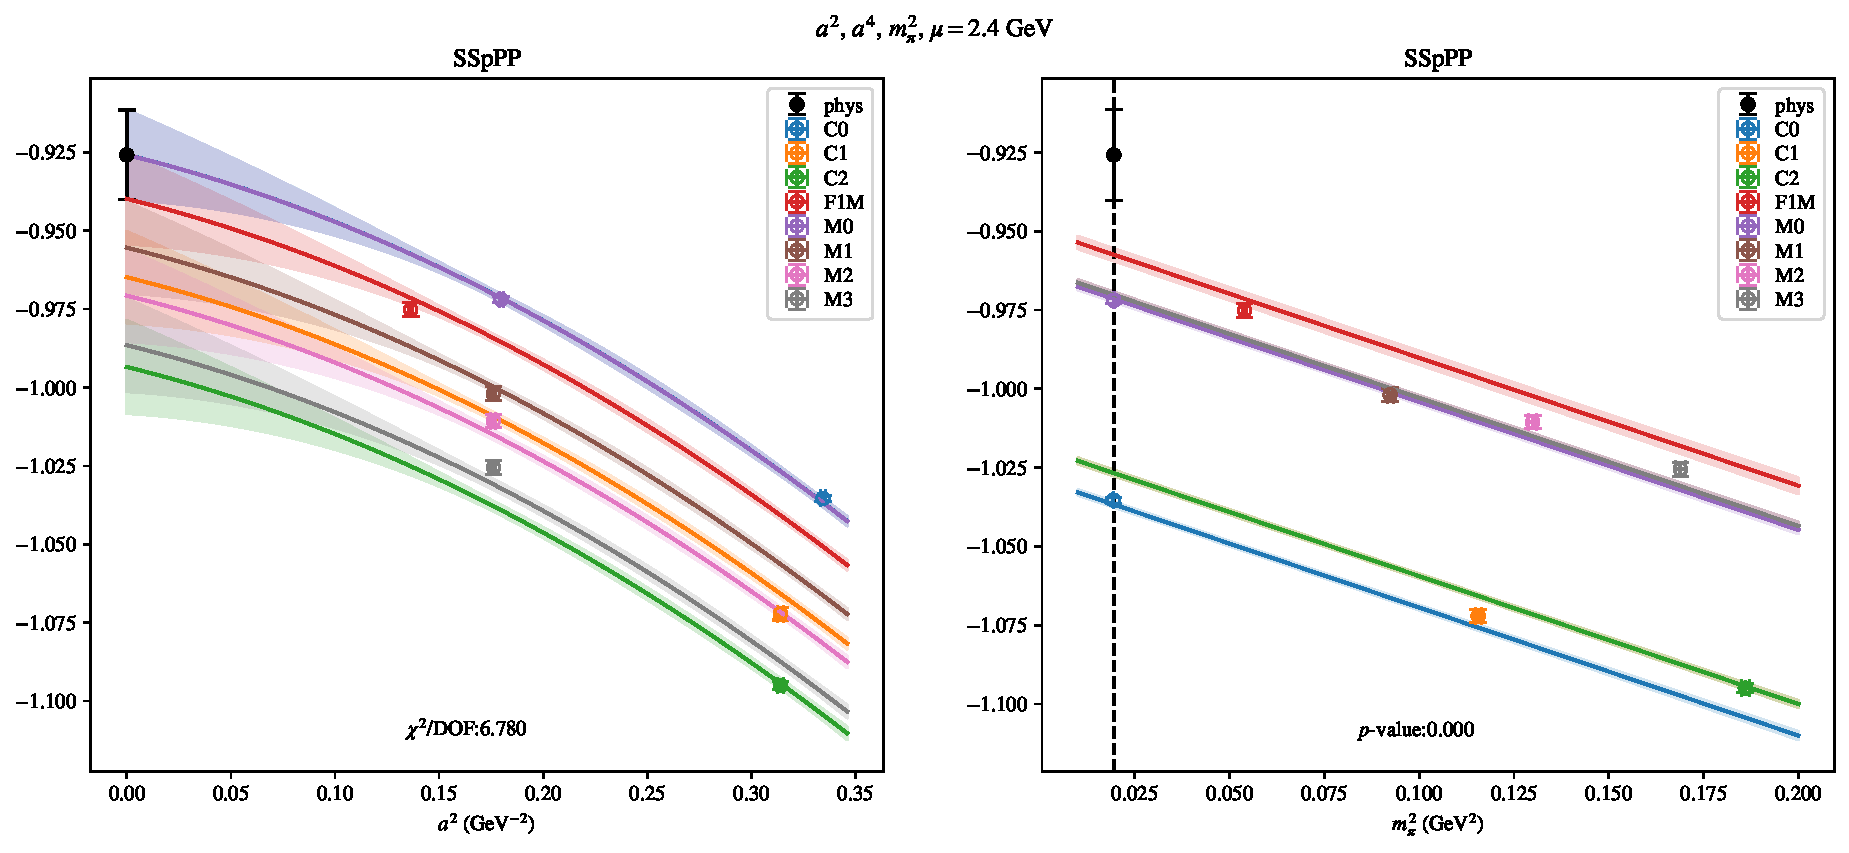
\includepdf[link, pages=-]{VVmAA/SUSY/a2a4m2_24.pdf}
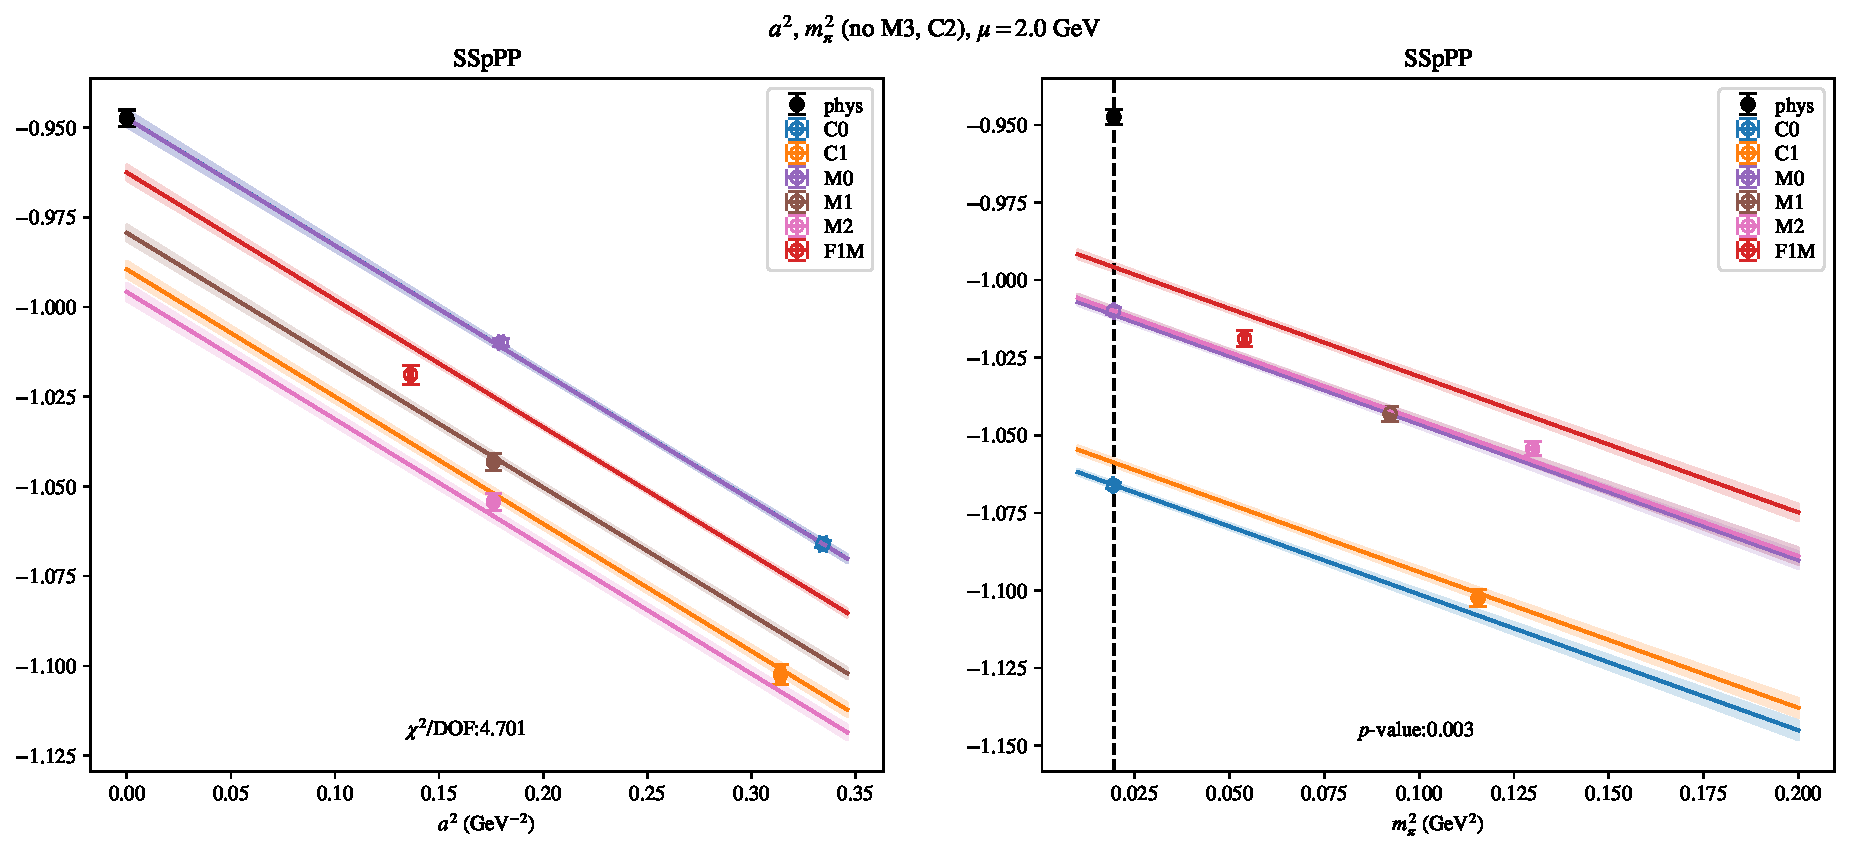
\includepdf[link, pages=-]{VVmAA/SUSY/a2m2mcut_20.pdf}
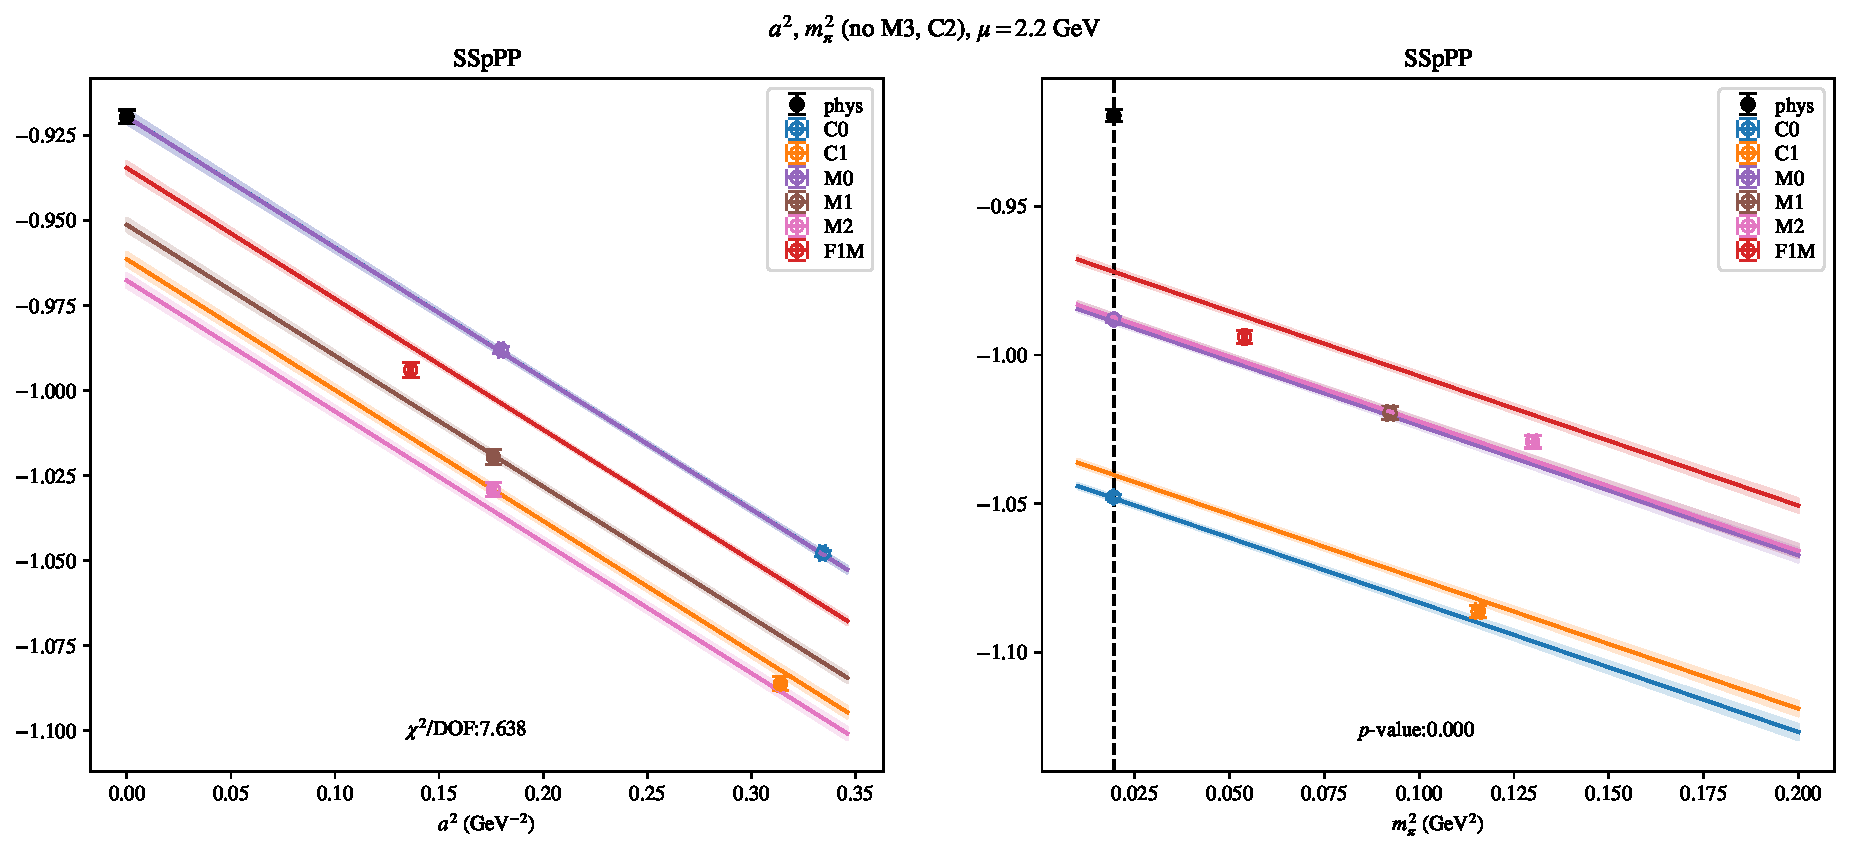
\includepdf[link, pages=-]{VVmAA/SUSY/a2m2mcut_22.pdf}
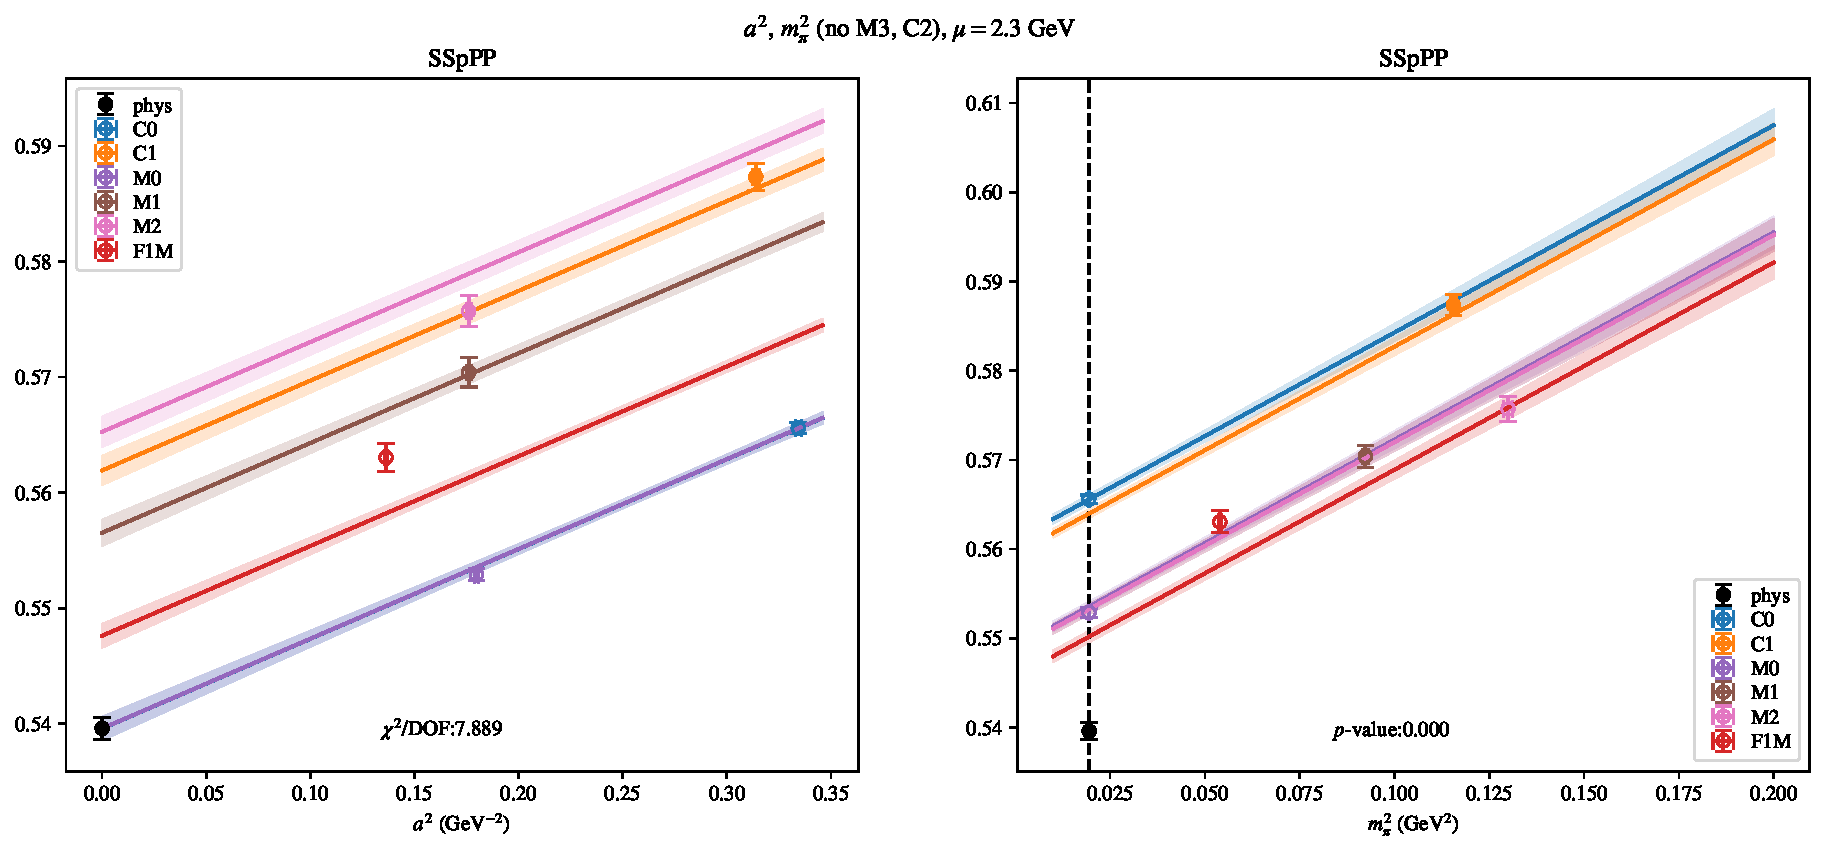
\includepdf[link, pages=-]{VVmAA/SUSY/a2m2mcut_23.pdf}
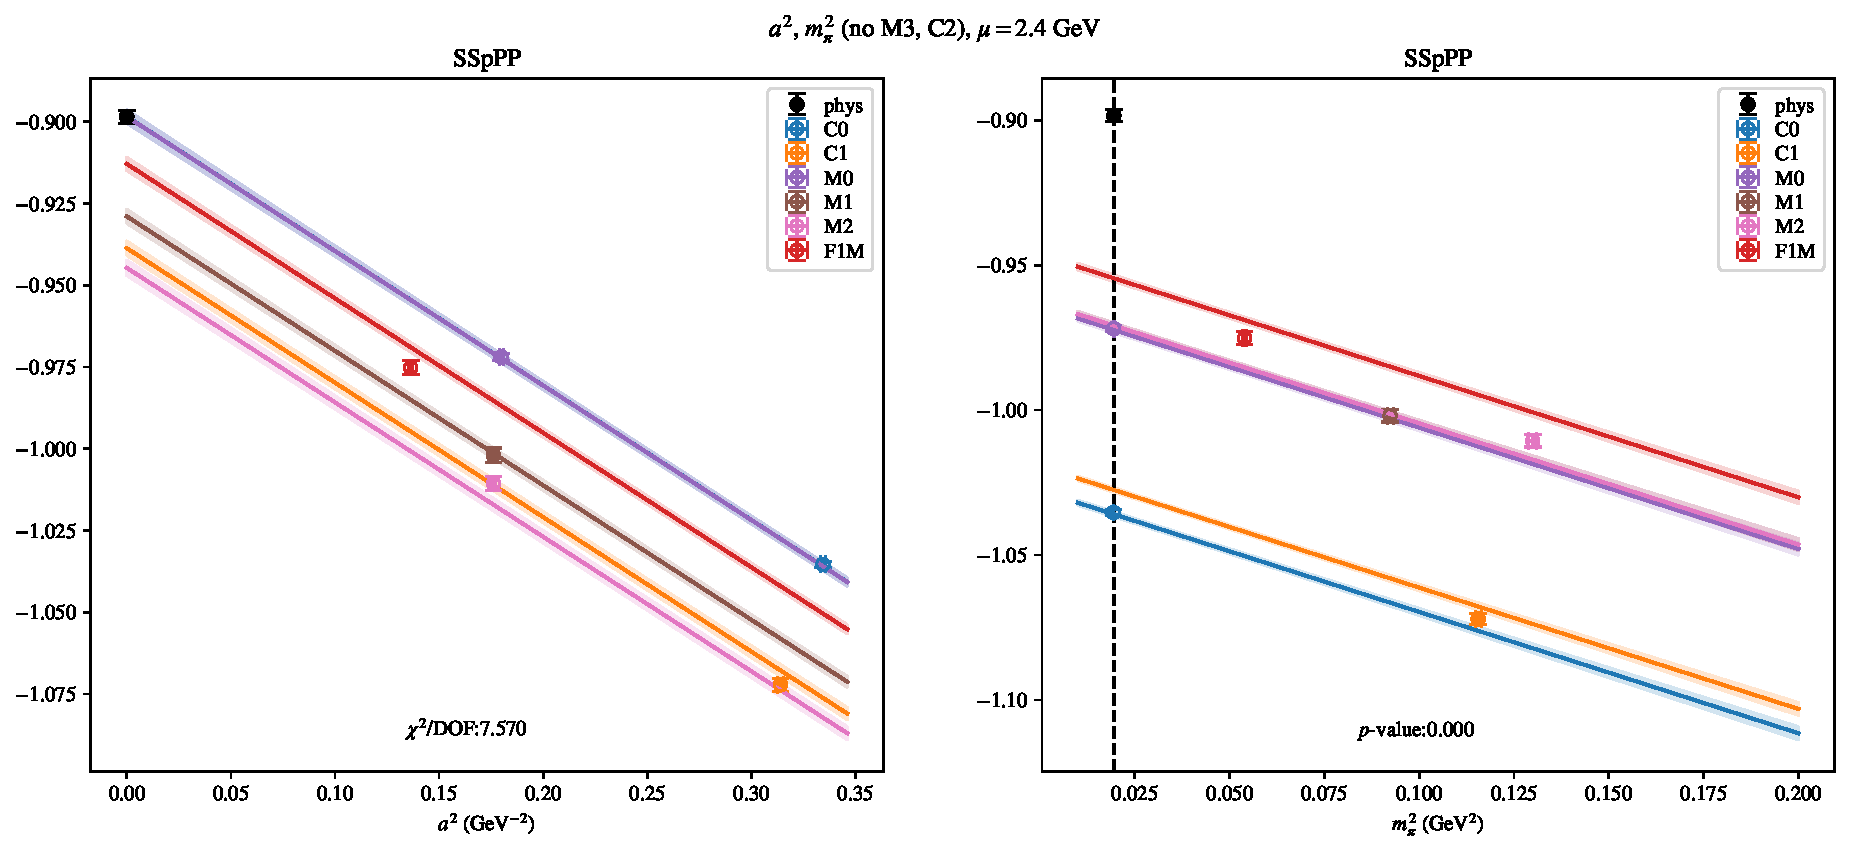
\includepdf[link, pages=-]{VVmAA/SUSY/a2m2mcut_24.pdf}
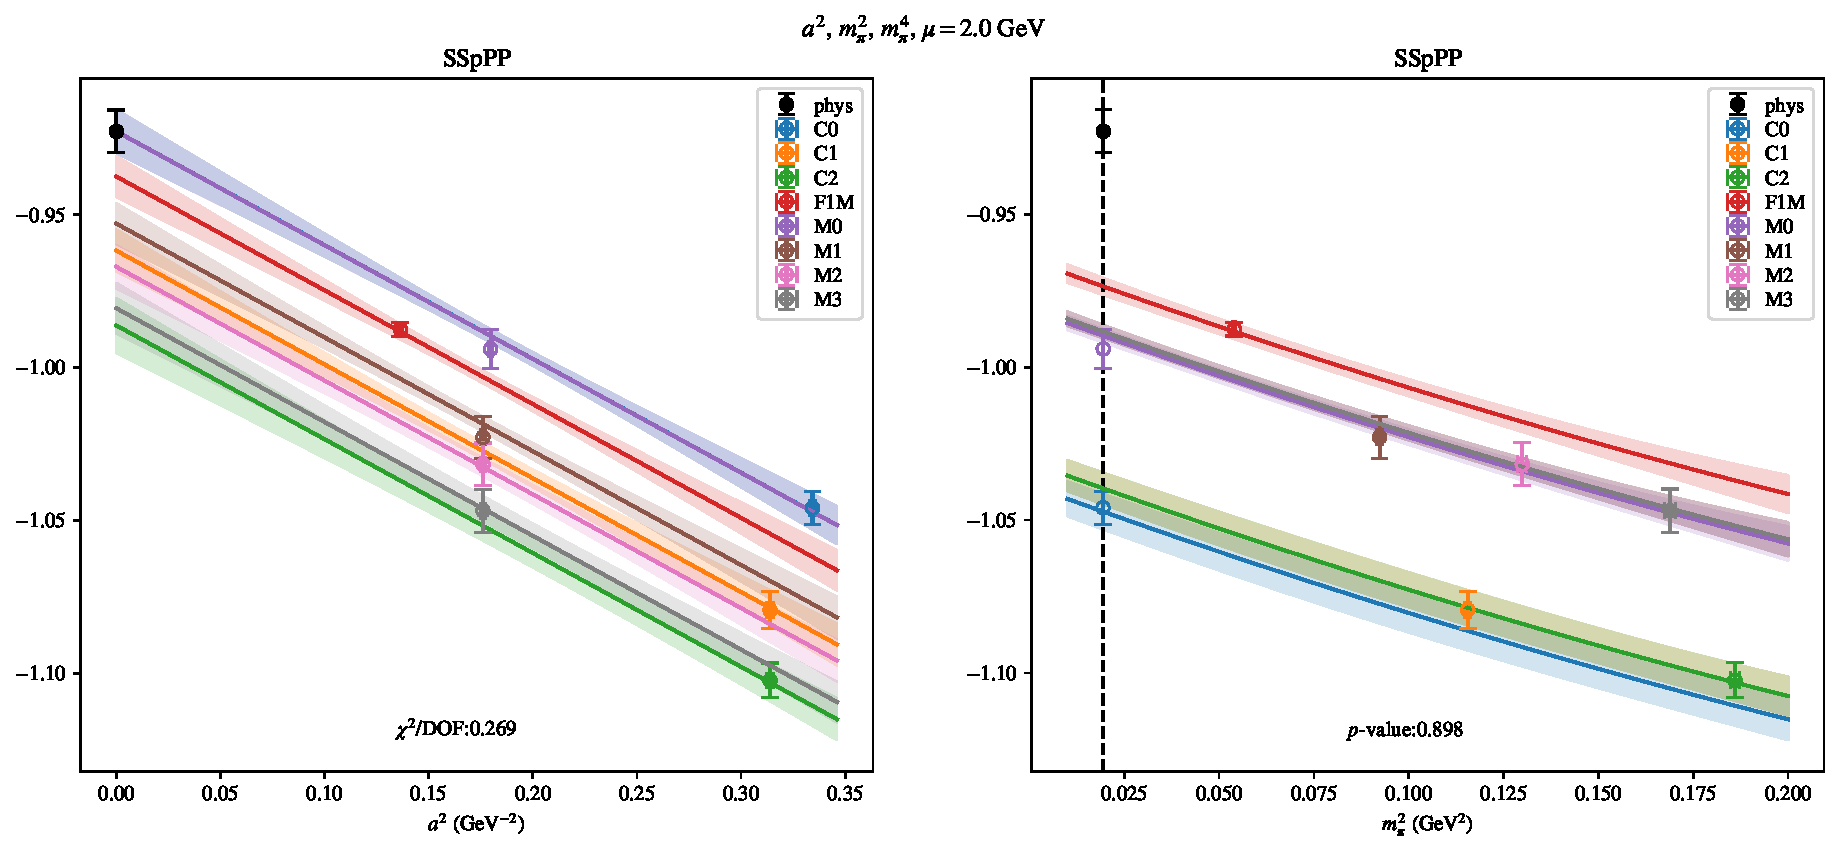
\includepdf[link, pages=-]{VVmAA/SUSY/a2m2m4_20.pdf}
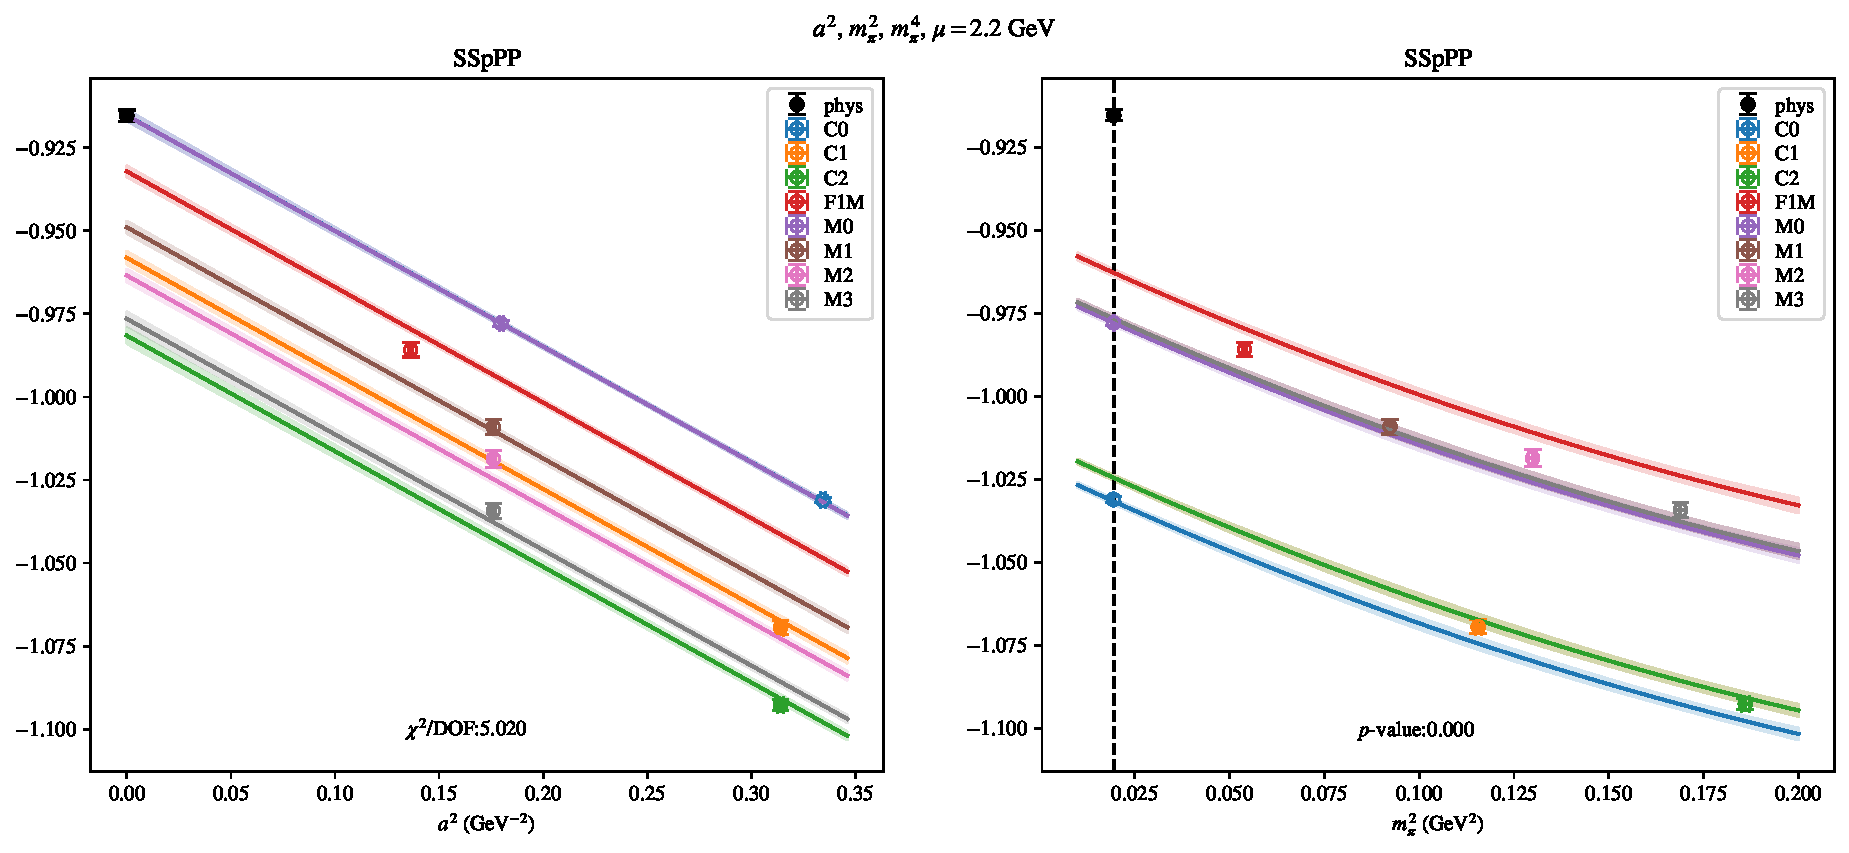
\includepdf[link, pages=-]{VVmAA/SUSY/a2m2m4_22.pdf}
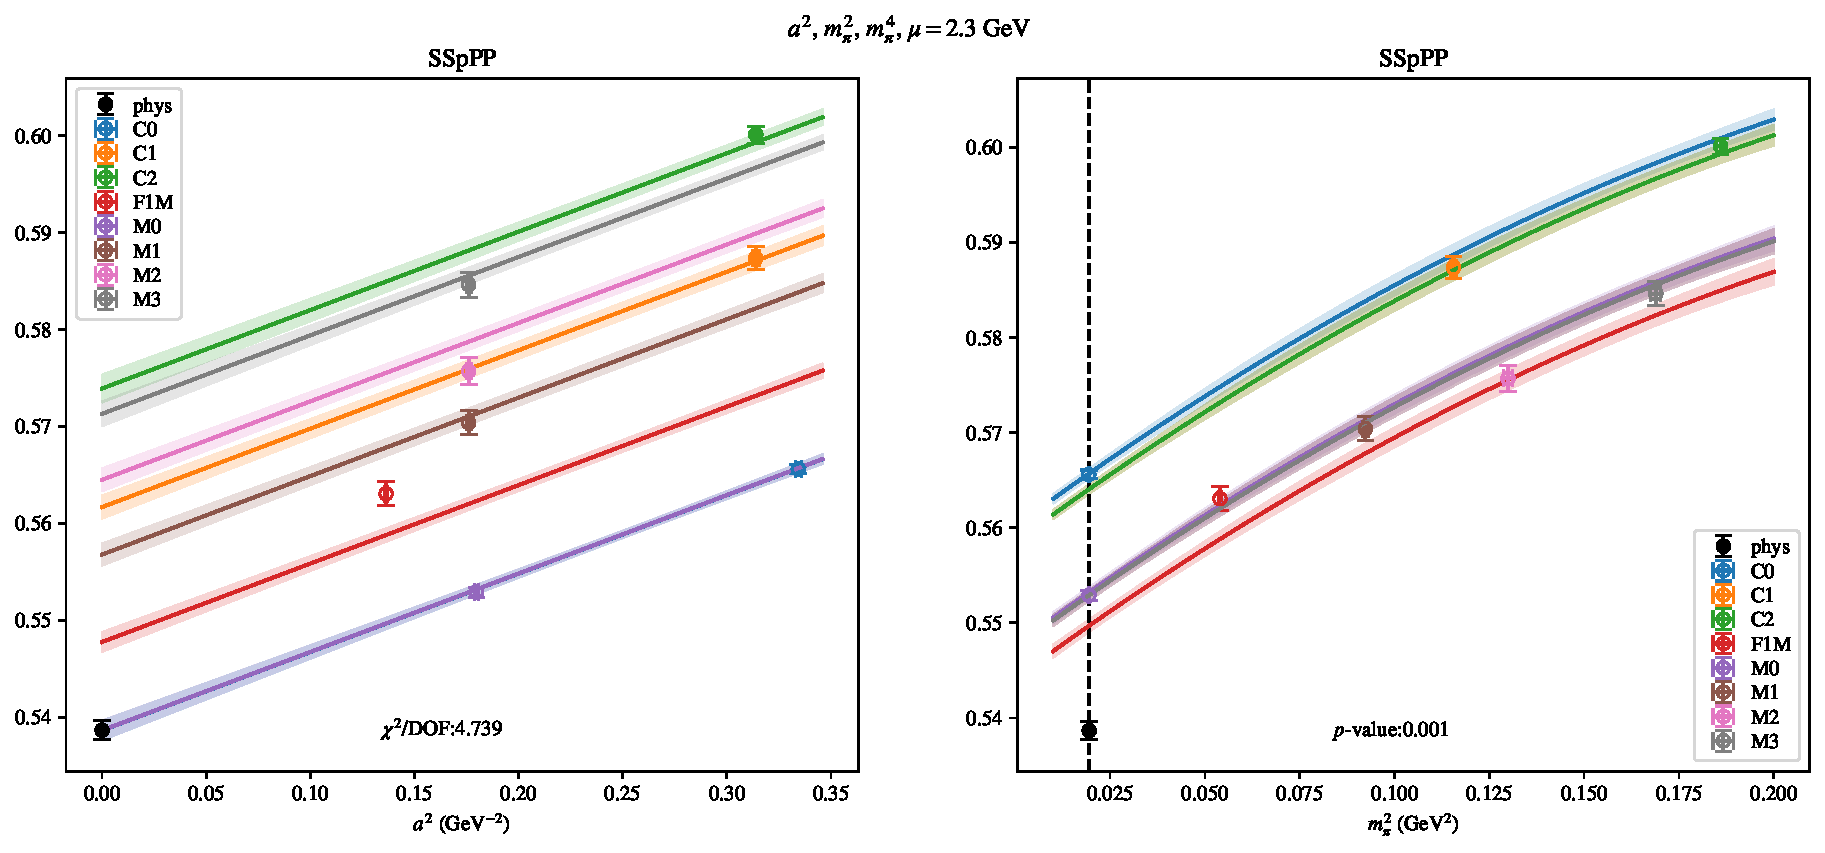
\includepdf[link, pages=-]{VVmAA/SUSY/a2m2m4_23.pdf}
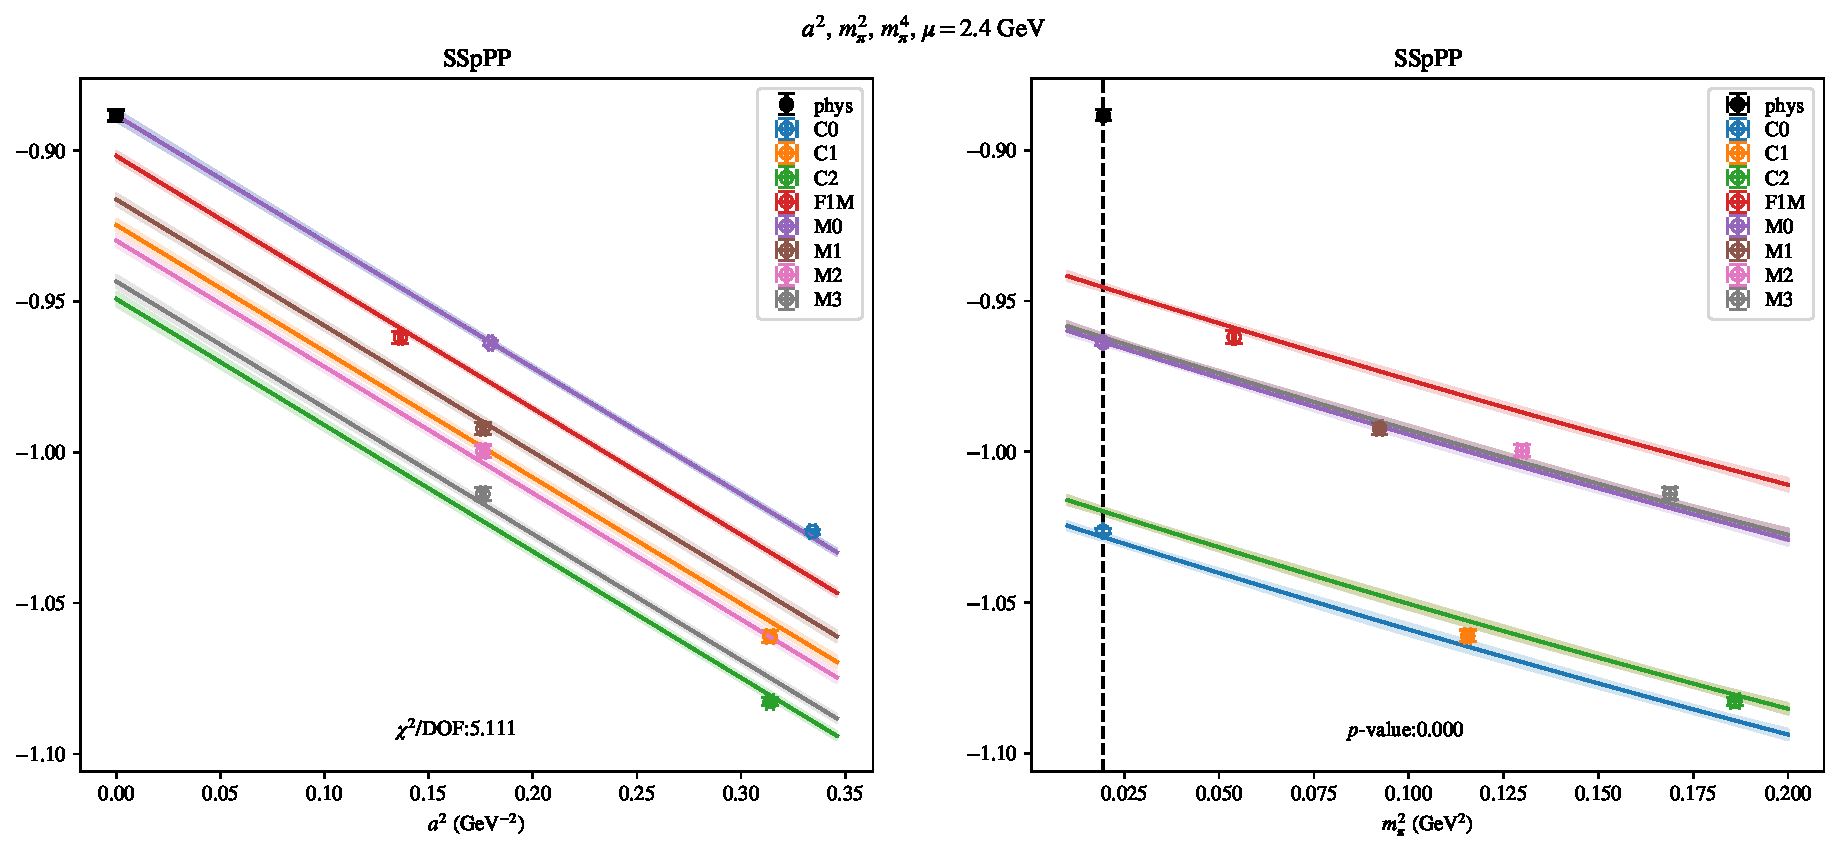
\includepdf[link, pages=-]{VVmAA/SUSY/a2m2m4_24.pdf}
\clearpage
\section{$B_3$}
\begin{table}[h!]
\begin{center}
\begin{tabular}{|c|c|c|c|c|c|}
\hline
$\mu$ (GeV) & $a^2$, $m_\pi^2$& $a^2$, $m_\pi^2$ (no C)& $a^2$, $a^4$, $m_\pi^2$& $a^2$, $m_\pi^2$ (no M3, C2)& $a^2$, $m_\pi^2$, $m_\pi^4$\\
\hline
2.0& \hyperlink{SSmPP/SUSY/a2m2_20.pdf.1}{\textbf{0.24441(54)}: 6.187 (0.0)} & \hyperlink{SSmPP/SUSY/a2m2noC_20.pdf.1}{\textbf{0.2439(30)}: 2.447 (0.087)} & \hyperlink{SSmPP/SUSY/a2a4m2_20.pdf.1}{\textbf{0.2318(50)}: 6.495 (0.0)} & \hyperlink{SSmPP/SUSY/a2m2mcut_20.pdf.1}{\textbf{0.24481(52)}: 7.55 (0.0)} & \hyperlink{SSmPP/SUSY/a2m2m4_20.pdf.1}{\textbf{0.24426(53)}: 7.67 (0.0)}\\
2.2& \hyperlink{SSmPP/SUSY/a2m2_22.pdf.1}{\textbf{0.23753(49)}: 9.848 (0.0)} & \hyperlink{SSmPP/SUSY/a2m2noC_22.pdf.1}{\textbf{0.2379(30)}: 3.368 (0.034)} & \hyperlink{SSmPP/SUSY/a2a4m2_22.pdf.1}{\textbf{0.2242(48)}: 10.548 (0.0)} & \hyperlink{SSmPP/SUSY/a2m2mcut_22.pdf.1}{\textbf{0.23803(50)}: 9.91 (0.0)} & \hyperlink{SSmPP/SUSY/a2m2m4_22.pdf.1}{\textbf{0.23726(50)}: 11.988 (0.0)}\\
2.3& \hyperlink{SSmPP/SUSY/a2m2_23.pdf.1}{\textbf{0.23437(46)}: 10.3 (0.0)} & \hyperlink{SSmPP/SUSY/a2m2noC_23.pdf.1}{\textbf{0.2355(29)}: 3.488 (0.031)} & \hyperlink{SSmPP/SUSY/a2a4m2_23.pdf.1}{\textbf{0.2221(47)}: 11.254 (0.0)} & \hyperlink{SSmPP/SUSY/a2m2mcut_23.pdf.1}{\textbf{0.23492(49)}: 10.301 (0.0)} & \hyperlink{SSmPP/SUSY/a2m2m4_23.pdf.1}{\textbf{0.23419(48)}: 12.705 (0.0)}\\
2.4& \hyperlink{SSmPP/SUSY/a2m2_24.pdf.1}{\textbf{0.23164(46)}: 12.882 (0.0)} & \hyperlink{SSmPP/SUSY/a2m2noC_24.pdf.1}{\textbf{0.2326(29)}: 3.433 (0.032)} & \hyperlink{SSmPP/SUSY/a2a4m2_24.pdf.1}{\textbf{0.2175(46)}: 13.845 (0.0)} & \hyperlink{SSmPP/SUSY/a2m2mcut_24.pdf.1}{\textbf{0.23237(49)}: 13.003 (0.0)} & \hyperlink{SSmPP/SUSY/a2m2m4_24.pdf.1}{\textbf{0.23155(48)}: 16.052 (0.0)}\\
\hline
\end{tabular}
\caption{Physical point value from chiral and continuum extrapolation at renormalisation scale $\mu$. Entries are \textbf{value(error)}: $\chi^2/\text{DOF}$ ($p$-value).}
\end{center}
\end{table}
\begin{table}[h!]
\begin{center}
\begin{tabular}{|c c|c|c|c|c|c|}
\hline
$\mu$ (GeV) &  & $a^2$, $m_\pi^2$& $a^2$, $m_\pi^2$ (no C)& $a^2$, $a^4$, $m_\pi^2$& $a^2$, $m_\pi^2$ (no M3, C2)& $a^2$, $m_\pi^2$, $m_\pi^4$\\
\hline
\multirow{2}{0.5in}{2.0} & $\alpha$ & 1.314(12)& 1.339(90)& 1.86(23)& 1.305(12)& 1.317(12)\\
 & $\beta$ & 0.01178(22)& 0.01036(43)& 0.01226(30)& 0.01190(36)& 0.01240(95)\\
\hline
\multirow{2}{0.5in}{2.2} & $\alpha$ & 1.394(12)& 1.397(90)& 2.00(23)& 1.382(12)& 1.399(12)\\
 & $\beta$ & 0.01140(20)& 0.00985(37)& 0.01189(28)& 0.01180(35)& 0.01265(93)\\
\hline
\multirow{2}{0.5in}{2.3} & $\alpha$ & 1.442(12)& 1.420(90)& 2.01(23)& 1.428(12)& 1.445(12)\\
 & $\beta$ & 0.01133(20)& 0.00976(35)& 0.01179(28)& 0.01157(33)& 0.01219(91)\\
\hline
\multirow{2}{0.5in}{2.4} & $\alpha$ & 1.487(13)& 1.472(91)& 2.15(24)& 1.470(13)& 1.489(13)\\
 & $\beta$ & 0.01138(18)& 0.00969(31)& 0.01192(27)& 0.01147(30)& 0.01182(86)\\
\hline
\end{tabular}
\caption{Fit values of coefficients in $B = B_{phys} + \mathbf{\alpha} a^2 + \mathbf{\beta}\left(\frac{m_\pi^2}{f_\pi^2}-\frac{m_{\pi,PDG}^2}{f_\pi^2}\right) + \ldots$.}
\end{center}
\end{table}
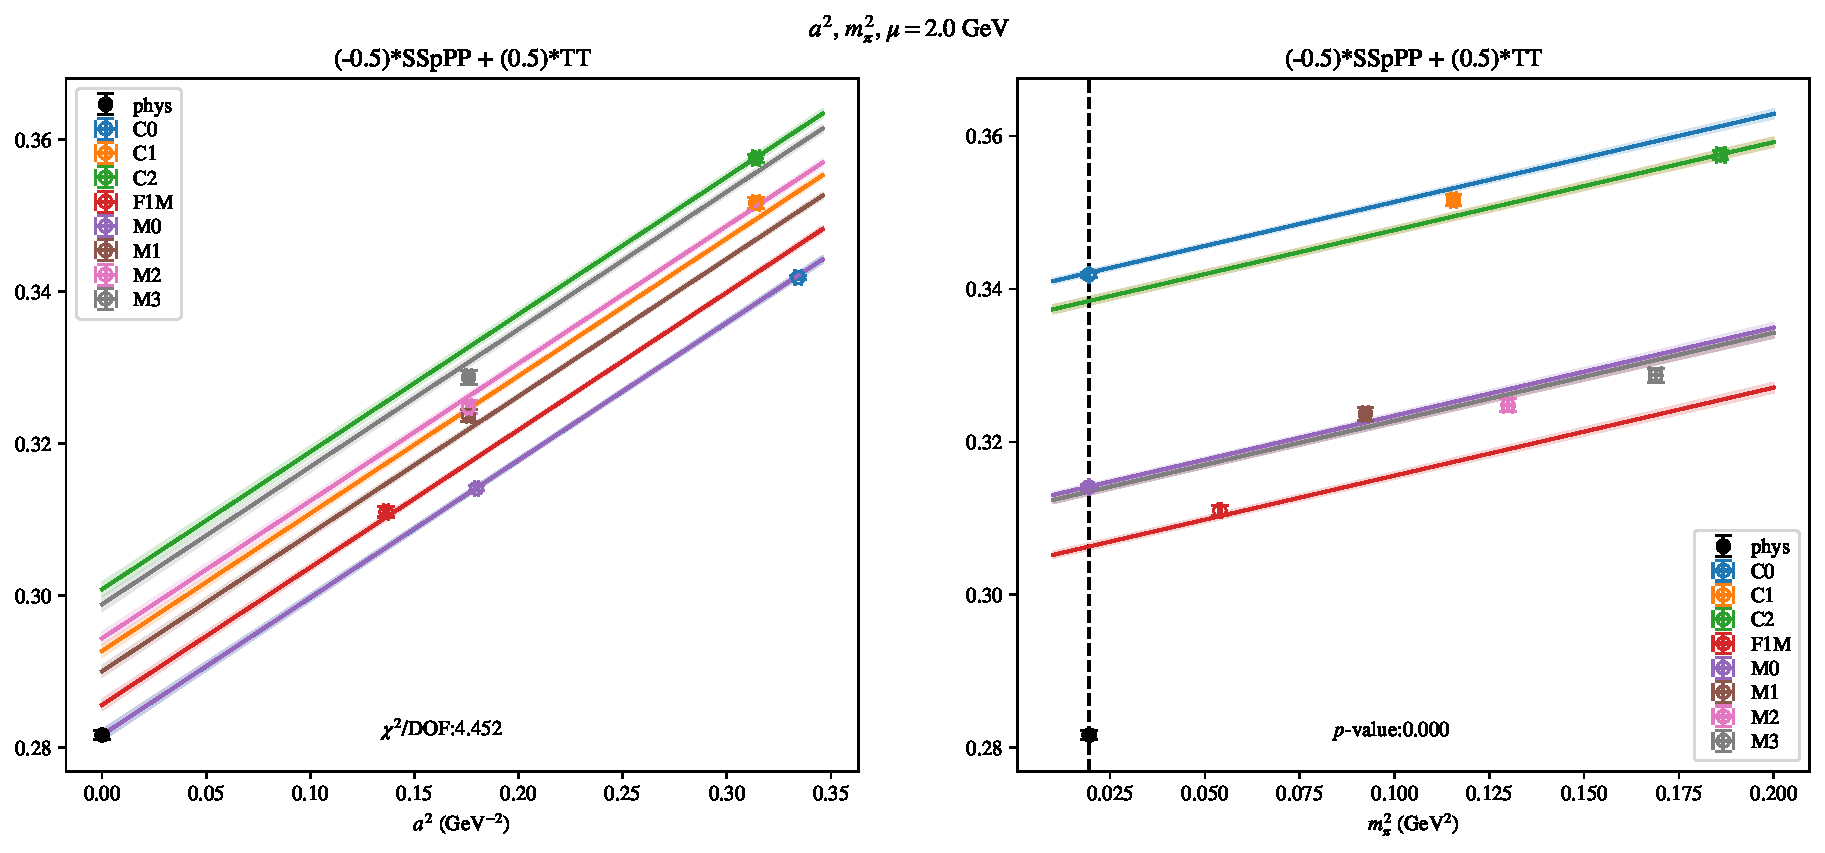
\includepdf[link, pages=-]{SSmPP/SUSY/a2m2_20.pdf}
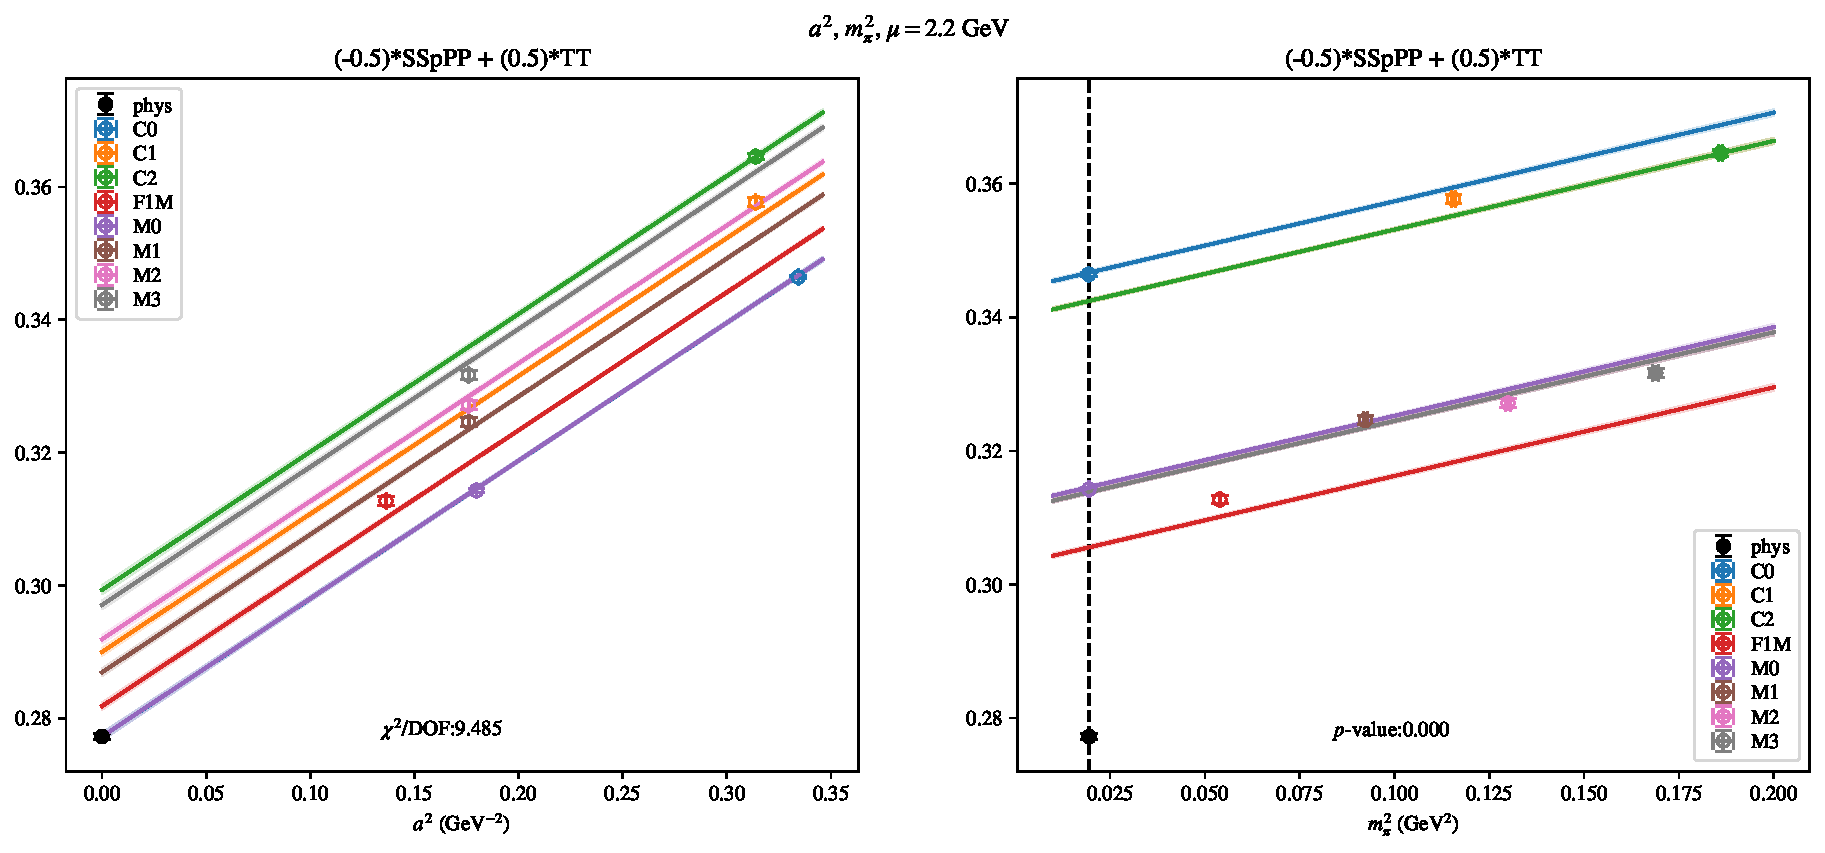
\includepdf[link, pages=-]{SSmPP/SUSY/a2m2_22.pdf}
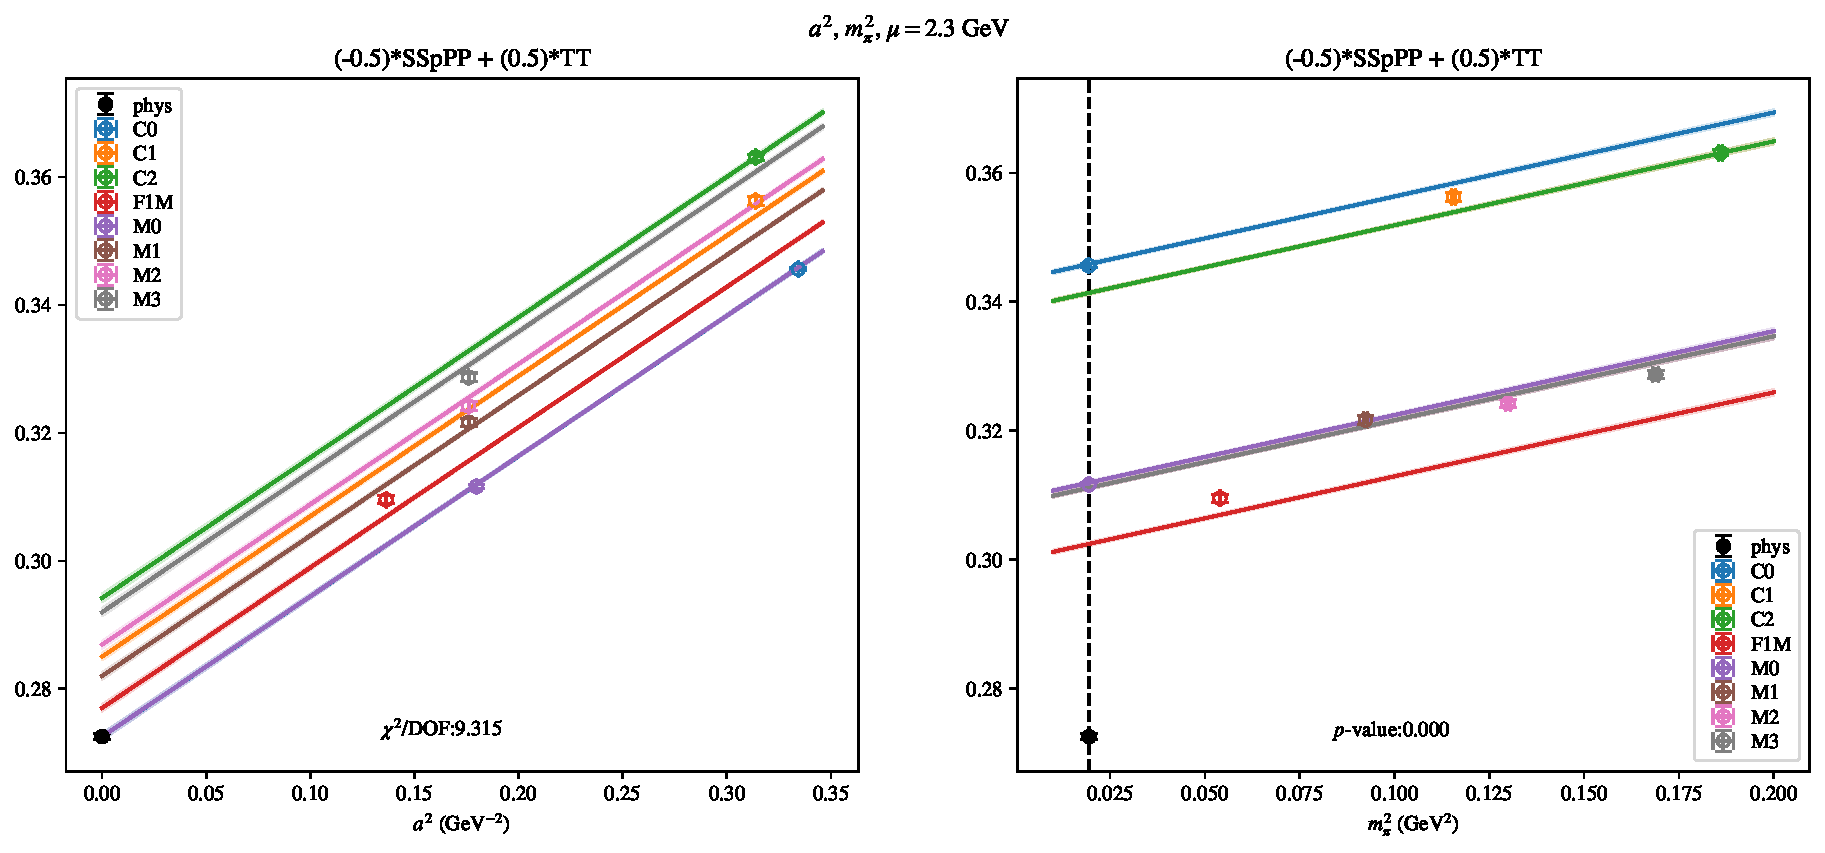
\includepdf[link, pages=-]{SSmPP/SUSY/a2m2_23.pdf}
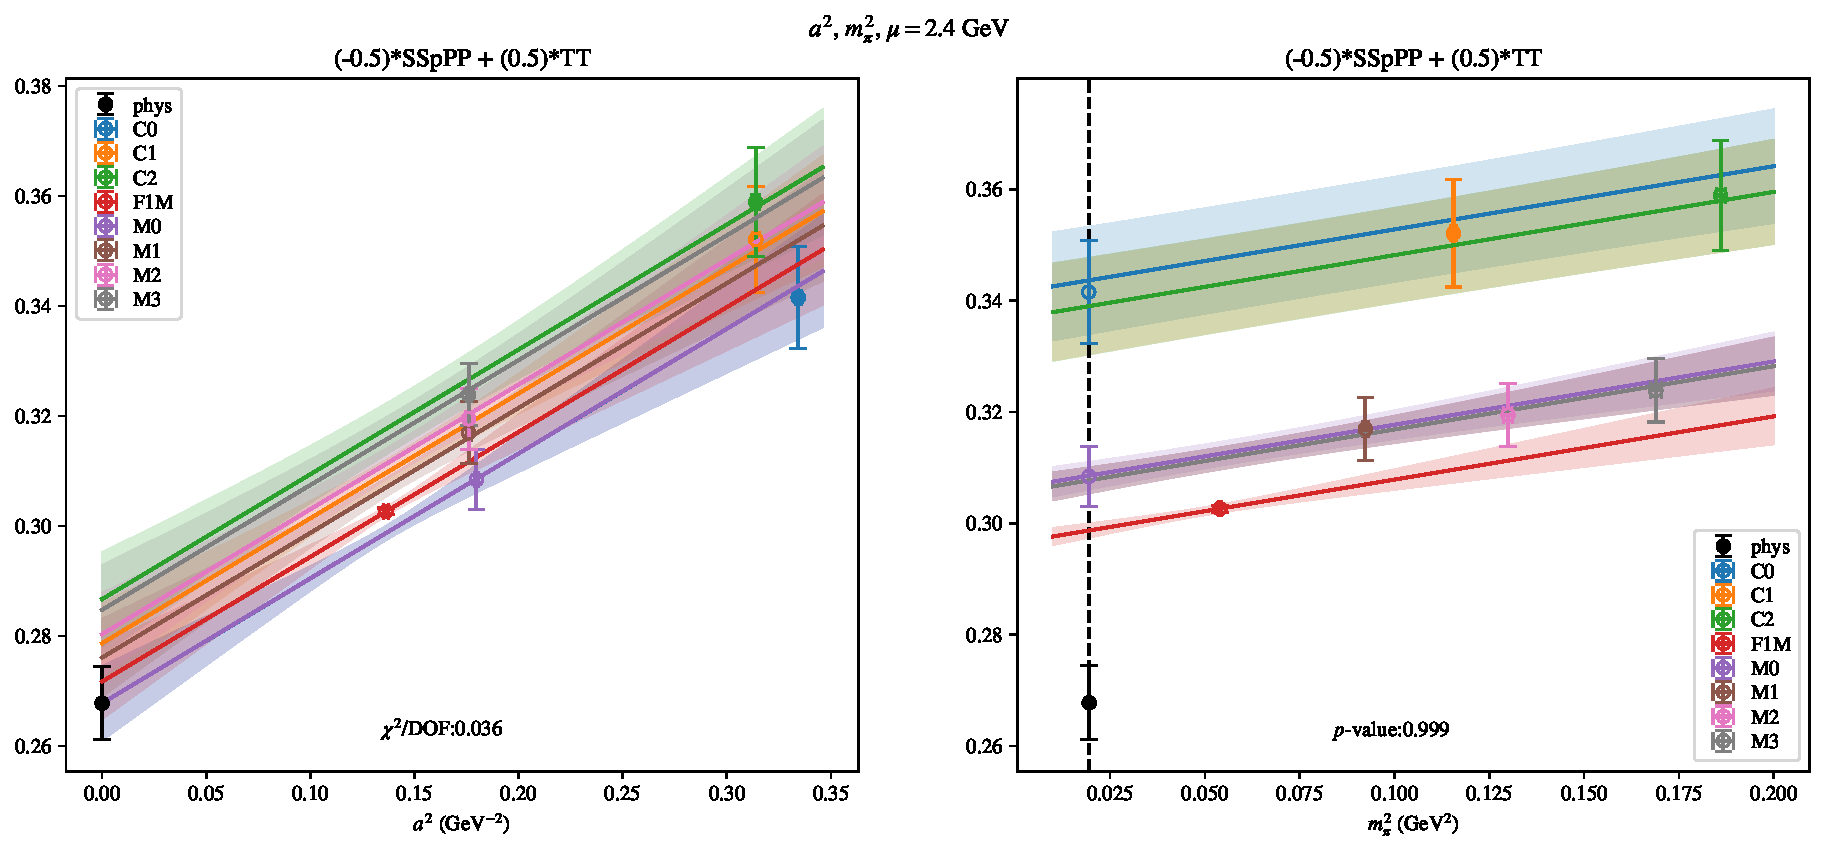
\includepdf[link, pages=-]{SSmPP/SUSY/a2m2_24.pdf}
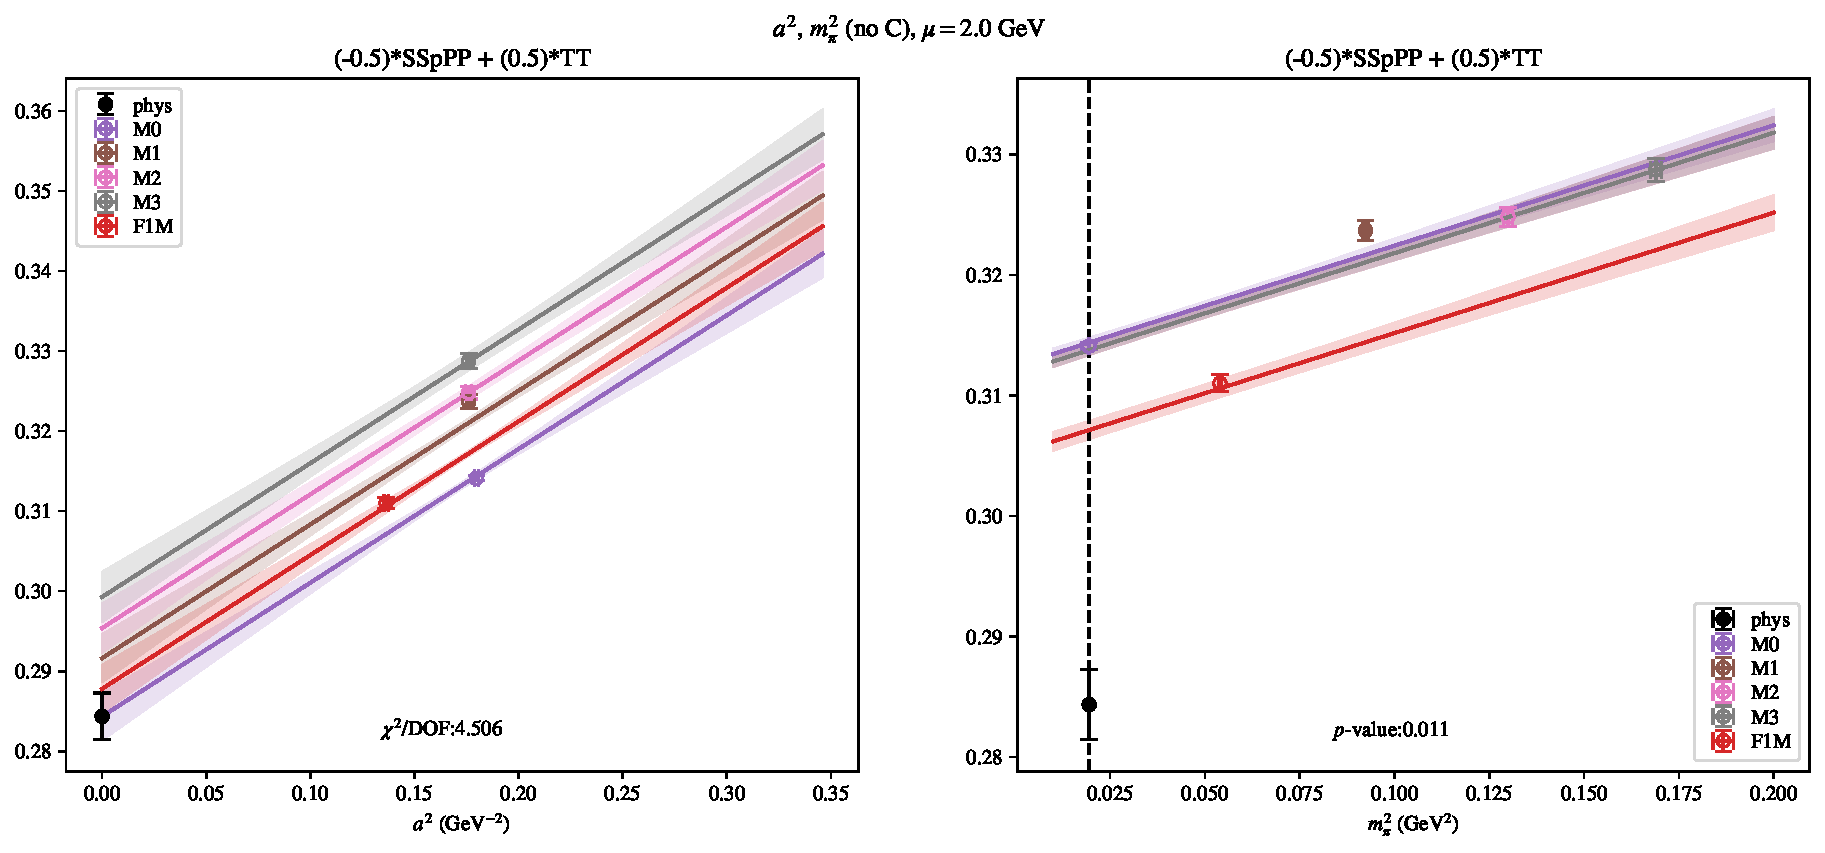
\includepdf[link, pages=-]{SSmPP/SUSY/a2m2noC_20.pdf}
\includepdf[link, pages=-]{SSmPP/SUSY/a2m2noC_22.pdf}
\includepdf[link, pages=-]{SSmPP/SUSY/a2m2noC_23.pdf}
\includepdf[link, pages=-]{SSmPP/SUSY/a2m2noC_24.pdf}
\includepdf[link, pages=-]{SSmPP/SUSY/a2a4m2_20.pdf}
\includepdf[link, pages=-]{SSmPP/SUSY/a2a4m2_22.pdf}
\includepdf[link, pages=-]{SSmPP/SUSY/a2a4m2_23.pdf}
\includepdf[link, pages=-]{SSmPP/SUSY/a2a4m2_24.pdf}
\includepdf[link, pages=-]{SSmPP/SUSY/a2m2mcut_20.pdf}
\includepdf[link, pages=-]{SSmPP/SUSY/a2m2mcut_22.pdf}
\includepdf[link, pages=-]{SSmPP/SUSY/a2m2mcut_23.pdf}
\includepdf[link, pages=-]{SSmPP/SUSY/a2m2mcut_24.pdf}
\includepdf[link, pages=-]{SSmPP/SUSY/a2m2m4_20.pdf}
\includepdf[link, pages=-]{SSmPP/SUSY/a2m2m4_22.pdf}
\includepdf[link, pages=-]{SSmPP/SUSY/a2m2m4_23.pdf}
\includepdf[link, pages=-]{SSmPP/SUSY/a2m2m4_24.pdf}
\clearpage
\section{$B_4$}
\begin{table}[h!]
\begin{center}
\begin{tabular}{|c|c|c|c|c|c|}
\hline
$\mu$ (GeV) & $a^2$, $m_\pi^2$& $a^2$, $m_\pi^2$ (no C)& $a^2$, $a^4$, $m_\pi^2$& $a^2$, $m_\pi^2$ (no M3, C2)& $a^2$, $m_\pi^2$, $m_\pi^4$\\
\hline
2.0& \hyperlink{SSpPP/SUSY/a2m2_20.pdf.1}{\textbf{1.8420(26)}: 5.573 (0.0)} & \hyperlink{SSpPP/SUSY/a2m2noC_20.pdf.1}{\textbf{1.784(13)}: 3.288 (0.037)} & \hyperlink{SSpPP/SUSY/a2a4m2_20.pdf.1}{\textbf{1.749(20)}: 2.007 (0.091)} & \hyperlink{SSpPP/SUSY/a2m2mcut_20.pdf.1}{\textbf{1.8426(29)}: 7.701 (0.0)} & \hyperlink{SSpPP/SUSY/a2m2m4_20.pdf.1}{\textbf{1.8458(28)}: 4.71 (0.001)}\\
2.2& \hyperlink{SSpPP/SUSY/a2m2_22.pdf.1}{\textbf{1.8335(25)}: 5.645 (0.0)} & \hyperlink{SSpPP/SUSY/a2m2noC_22.pdf.1}{\textbf{1.772(12)}: 1.987 (0.137)} & \hyperlink{SSpPP/SUSY/a2a4m2_22.pdf.1}{\textbf{1.734(20)}: 1.301 (0.267)} & \hyperlink{SSpPP/SUSY/a2m2mcut_22.pdf.1}{\textbf{1.8340(28)}: 8.299 (0.0)} & \hyperlink{SSpPP/SUSY/a2m2m4_22.pdf.1}{\textbf{1.8369(28)}: 5.233 (0.0)}\\
2.3& \hyperlink{SSpPP/SUSY/a2m2_23.pdf.1}{\textbf{1.8302(25)}: 5.986 (0.0)} & \hyperlink{SSpPP/SUSY/a2m2noC_23.pdf.1}{\textbf{1.767(12)}: 2.109 (0.121)} & \hyperlink{SSpPP/SUSY/a2a4m2_23.pdf.1}{\textbf{1.729(20)}: 1.467 (0.209)} & \hyperlink{SSpPP/SUSY/a2m2mcut_23.pdf.1}{\textbf{1.8308(27)}: 8.806 (0.0)} & \hyperlink{SSpPP/SUSY/a2m2m4_23.pdf.1}{\textbf{1.8338(28)}: 5.471 (0.0)}\\
2.4& \hyperlink{SSpPP/SUSY/a2m2_24.pdf.1}{\textbf{1.8279(25)}: 6.734 (0.0)} & \hyperlink{SSpPP/SUSY/a2m2noC_24.pdf.1}{\textbf{1.762(12)}: 2.436 (0.087)} & \hyperlink{SSpPP/SUSY/a2a4m2_24.pdf.1}{\textbf{1.721(20)}: 1.638 (0.161)} & \hyperlink{SSpPP/SUSY/a2m2mcut_24.pdf.1}{\textbf{1.8287(28)}: 9.927 (0.0)} & \hyperlink{SSpPP/SUSY/a2m2m4_24.pdf.1}{\textbf{1.8319(28)}: 6.112 (0.0)}\\
\hline
\end{tabular}
\caption{Physical point value from chiral and continuum extrapolation at renormalisation scale $\mu$. Entries are \textbf{value(error)}: $\chi^2/\text{DOF}$ ($p$-value).}
\end{center}
\end{table}
\begin{table}[h!]
\begin{center}
\begin{tabular}{|c c|c|c|c|c|c|}
\hline
$\mu$ (GeV) &  & $a^2$, $m_\pi^2$& $a^2$, $m_\pi^2$ (no C)& $a^2$, $a^4$, $m_\pi^2$& $a^2$, $m_\pi^2$ (no M3, C2)& $a^2$, $m_\pi^2$, $m_\pi^4$\\
\hline
\multirow{2}{0.5in}{2.0} & $\alpha$ & 0.0699(54)& 0.260(43)& 0.55(11)& 0.0691(60)& 0.0629(59)\\
 & $\beta$ & 0.0& 0.00010(23)& -0.0& -0.0002(23)& -0.0018(63)\\
\hline
\multirow{2}{0.5in}{2.2} & $\alpha$ & 0.0713(53)& 0.273(42)& 0.58(11)& 0.0707(58)& 0.0651(58)\\
 & $\beta$ & -0.0002(12)& -0.0002(22)& -0.0004(13)& -0.0004(23)& -0.0019(66)\\
\hline
\multirow{2}{0.5in}{2.3} & $\alpha$ & 0.0729(53)& 0.281(43)& 0.60(11)& 0.0721(58)& 0.0662(58)\\
 & $\beta$ & -0.0002(11)& -0.0002(21)& -0.0004(13)& -0.0005(22)& -0.0020(64)\\
\hline
\multirow{2}{0.5in}{2.4} & $\alpha$ & 0.0737(53)& 0.293(43)& 0.63(11)& 0.0726(58)& 0.0665(58)\\
 & $\beta$ & -0.0002(11)& -0.0003(20)& -0.0005(12)& -0.0005(20)& -0.0021(62)\\
\hline
\end{tabular}
\caption{Fit values of coefficients in $B = B_{phys} + \mathbf{\alpha} a^2 + \mathbf{\beta}\left(\frac{m_\pi^2}{f_\pi^2}-\frac{m_{\pi,PDG}^2}{f_\pi^2}\right) + \ldots$.}
\end{center}
\end{table}
\includepdf[link, pages=-]{SSpPP/SUSY/a2m2_20.pdf}
\includepdf[link, pages=-]{SSpPP/SUSY/a2m2_22.pdf}
\includepdf[link, pages=-]{SSpPP/SUSY/a2m2_23.pdf}
\includepdf[link, pages=-]{SSpPP/SUSY/a2m2_24.pdf}
\includepdf[link, pages=-]{SSpPP/SUSY/a2m2noC_20.pdf}
\includepdf[link, pages=-]{SSpPP/SUSY/a2m2noC_22.pdf}
\includepdf[link, pages=-]{SSpPP/SUSY/a2m2noC_23.pdf}
\includepdf[link, pages=-]{SSpPP/SUSY/a2m2noC_24.pdf}
\includepdf[link, pages=-]{SSpPP/SUSY/a2a4m2_20.pdf}
\includepdf[link, pages=-]{SSpPP/SUSY/a2a4m2_22.pdf}
\includepdf[link, pages=-]{SSpPP/SUSY/a2a4m2_23.pdf}
\includepdf[link, pages=-]{SSpPP/SUSY/a2a4m2_24.pdf}
\includepdf[link, pages=-]{SSpPP/SUSY/a2m2mcut_20.pdf}
\includepdf[link, pages=-]{SSpPP/SUSY/a2m2mcut_22.pdf}
\includepdf[link, pages=-]{SSpPP/SUSY/a2m2mcut_23.pdf}
\includepdf[link, pages=-]{SSpPP/SUSY/a2m2mcut_24.pdf}
\includepdf[link, pages=-]{SSpPP/SUSY/a2m2m4_20.pdf}
\includepdf[link, pages=-]{SSpPP/SUSY/a2m2m4_22.pdf}
\includepdf[link, pages=-]{SSpPP/SUSY/a2m2m4_23.pdf}
\includepdf[link, pages=-]{SSpPP/SUSY/a2m2m4_24.pdf}
\clearpage
\section{$B_5$}
\begin{table}[h!]
\begin{center}
\begin{tabular}{|c|c|c|c|c|c|}
\hline
$\mu$ (GeV) & $a^2$, $m_\pi^2$& $a^2$, $m_\pi^2$ (no C)& $a^2$, $a^4$, $m_\pi^2$& $a^2$, $m_\pi^2$ (no M3, C2)& $a^2$, $m_\pi^2$, $m_\pi^4$\\
\hline
2.0& \hyperlink{TT/SUSY/a2m2_20.pdf.1}{\textbf{0.50687(70)}: 5.414 (0.0)} & \hyperlink{TT/SUSY/a2m2noC_20.pdf.1}{\textbf{0.4904(45)}: 6.607 (0.001)} & \hyperlink{TT/SUSY/a2a4m2_20.pdf.1}{\textbf{0.4827(68)}: 3.812 (0.004)} & \hyperlink{TT/SUSY/a2m2mcut_20.pdf.1}{\textbf{0.50704(76)}: 7.087 (0.0)} & \hyperlink{TT/SUSY/a2m2m4_20.pdf.1}{\textbf{0.50776(74)}: 4.164 (0.002)}\\
2.2& \hyperlink{TT/SUSY/a2m2_22.pdf.1}{\textbf{0.51017(67)}: 4.823 (0.0)} & \hyperlink{TT/SUSY/a2m2noC_22.pdf.1}{\textbf{0.4933(43)}: 4.28 (0.014)} & \hyperlink{TT/SUSY/a2a4m2_22.pdf.1}{\textbf{0.4853(65)}: 2.652 (0.031)} & \hyperlink{TT/SUSY/a2m2mcut_22.pdf.1}{\textbf{0.51030(72)}: 6.129 (0.0)} & \hyperlink{TT/SUSY/a2m2m4_22.pdf.1}{\textbf{0.51098(71)}: 3.932 (0.003)}\\
2.3& \hyperlink{TT/SUSY/a2m2_23.pdf.1}{\textbf{0.51183(67)}: 5.2 (0.0)} & \hyperlink{TT/SUSY/a2m2noC_23.pdf.1}{\textbf{0.4941(43)}: 4.273 (0.014)} & \hyperlink{TT/SUSY/a2a4m2_23.pdf.1}{\textbf{0.4859(64)}: 2.758 (0.026)} & \hyperlink{TT/SUSY/a2m2mcut_23.pdf.1}{\textbf{0.51198(71)}: 6.723 (0.0)} & \hyperlink{TT/SUSY/a2m2m4_23.pdf.1}{\textbf{0.51268(70)}: 4.271 (0.002)}\\
2.4& \hyperlink{TT/SUSY/a2m2_24.pdf.1}{\textbf{0.51328(66)}: 5.588 (0.0)} & \hyperlink{TT/SUSY/a2m2noC_24.pdf.1}{\textbf{0.4951(42)}: 4.6 (0.01)} & \hyperlink{TT/SUSY/a2a4m2_24.pdf.1}{\textbf{0.4871(64)}: 3.091 (0.015)} & \hyperlink{TT/SUSY/a2m2mcut_24.pdf.1}{\textbf{0.51341(71)}: 7.129 (0.0)} & \hyperlink{TT/SUSY/a2m2m4_24.pdf.1}{\textbf{0.51416(70)}: 4.625 (0.001)}\\
\hline
\end{tabular}
\caption{Physical point value from chiral and continuum extrapolation at renormalisation scale $\mu$. Entries are \textbf{value(error)}: $\chi^2/\text{DOF}$ ($p$-value).}
\end{center}
\end{table}
\begin{table}[h!]
\begin{center}
\begin{tabular}{|c c|c|c|c|c|c|}
\hline
$\mu$ (GeV) &  & $a^2$, $m_\pi^2$& $a^2$, $m_\pi^2$ (no C)& $a^2$, $a^4$, $m_\pi^2$& $a^2$, $m_\pi^2$ (no M3, C2)& $a^2$, $m_\pi^2$, $m_\pi^4$\\
\hline
\multirow{2}{0.5in}{2.0} & $\alpha$ & -0.180(54)& 0.004& 0.25(12)& -0.181(58)& -0.186(56)\\
 & $\beta$ & 0.00217(16)& 0.00229(26)& 0.00214(17)& 0.00178(26)& 0.0\\
\hline
\multirow{2}{0.5in}{2.2} & $\alpha$ & -0.225(49)& -0.03(49)& 0.21(12)& -0.225(54)& -0.230(53)\\
 & $\beta$ & 0.00169(13)& 0.00180(24)& 0.00162(14)& 0.00132(25)& -0.0001(71)\\
\hline
\multirow{2}{0.5in}{2.3} & $\alpha$ & -0.247(48)& -0.05(49)& 0.20(12)& -0.248(53)& -0.252(52)\\
 & $\beta$ & 0.00158(12)& 0.00168(22)& 0.00150(13)& 0.00122(23)& -0.0002(66)\\
\hline
\multirow{2}{0.5in}{2.4} & $\alpha$ & -0.268(49)& -0.06(48)& 0.19(12)& -0.268(53)& -0.273(52)\\
 & $\beta$ & 0.00147(12)& 0.00159(21)& 0.00138(12)& 0.00111(21)& -0.0003(64)\\
\hline
\end{tabular}
\caption{Fit values of coefficients in $B = B_{phys} + \mathbf{\alpha} a^2 + \mathbf{\beta}\left(\frac{m_\pi^2}{f_\pi^2}-\frac{m_{\pi,PDG}^2}{f_\pi^2}\right) + \ldots$.}
\end{center}
\end{table}
\includepdf[link, pages=-]{TT/SUSY/a2m2_20.pdf}
\includepdf[link, pages=-]{TT/SUSY/a2m2_22.pdf}
\includepdf[link, pages=-]{TT/SUSY/a2m2_23.pdf}
\includepdf[link, pages=-]{TT/SUSY/a2m2_24.pdf}
\includepdf[link, pages=-]{TT/SUSY/a2m2noC_20.pdf}
\includepdf[link, pages=-]{TT/SUSY/a2m2noC_22.pdf}
\includepdf[link, pages=-]{TT/SUSY/a2m2noC_23.pdf}
\includepdf[link, pages=-]{TT/SUSY/a2m2noC_24.pdf}
\includepdf[link, pages=-]{TT/SUSY/a2a4m2_20.pdf}
\includepdf[link, pages=-]{TT/SUSY/a2a4m2_22.pdf}
\includepdf[link, pages=-]{TT/SUSY/a2a4m2_23.pdf}
\includepdf[link, pages=-]{TT/SUSY/a2a4m2_24.pdf}
\includepdf[link, pages=-]{TT/SUSY/a2m2mcut_20.pdf}
\includepdf[link, pages=-]{TT/SUSY/a2m2mcut_22.pdf}
\includepdf[link, pages=-]{TT/SUSY/a2m2mcut_23.pdf}
\includepdf[link, pages=-]{TT/SUSY/a2m2mcut_24.pdf}
\includepdf[link, pages=-]{TT/SUSY/a2m2m4_20.pdf}
\includepdf[link, pages=-]{TT/SUSY/a2m2m4_22.pdf}
\includepdf[link, pages=-]{TT/SUSY/a2m2m4_23.pdf}
\includepdf[link, pages=-]{TT/SUSY/a2m2m4_24.pdf}
\clearpage
\end{document}